\documentclass[11pt]{amsart}
\usepackage[utf8]{inputenc}
\usepackage[T1]{fontenc}
\allowdisplaybreaks
\usepackage{hyperref}
\hypersetup{
  colorlinks   = true, % Colours links instead of ugly boxes
  urlcolor     = {blue!80!black}, % Colour for external hyperlinks
  linkcolor    = {red!80!black}, % Colour of internal links
  citecolor   = {blue!50!black} % Colour of citations	
}
\usepackage[left=0.8in,right=0.8in,top=1in,bottom=1in]{geometry}
\usepackage{amsmath, amsthm, amssymb, amsfonts, amsthm, bbold, bm, xcolor}
\usepackage{adjustbox}
\usepackage{tikz, tikz-cd, float, paralist, pgfplots, tcolorbox, subfig, filecontents}
\usepackage[pdftex,outline]{contour}
\usepgfplotslibrary{fillbetween}
\usetikzlibrary{arrows}
\usetikzlibrary{shapes.geometric}
\usepackage[nobysame]{amsrefs}
\usepackage{tgpagella}
\usepackage{pdiag}

% Algorithm package
% \usepackage[linesnumbered,lined,boxed,vlined,ruled]{algorithm2e}
\usepackage[lined,boxed,vlined,ruled]{algorithm2e}
\SetKw{Continue}{continue}
\SetKw{Or}{or}
\SetKw{Until}{until}
% Set the algorithm comments to blue
\newcommand\mycommfont[1]{\ttfamily\textcolor{blue}{#1}}
\SetCommentSty{mycommfont}
% \SetAlFnt{\large}
% \SetAlCapFnt{\large}
% \SetAlCapNameFnt{\large}
% \SetProcFnt{\Large}

\DeclareMathOperator*{\argmin}{\arg\min}

\newcommand{\nc}{\newcommand}
\newcommand{\rc}{\renewcommand}
\nc{\on}{\operatorname}

% Commands 
\rc{\AA}{\mathbb{A}}	\nc{\calA}{\mathcal{A}}	\nc{\fraka}{\mathfrak{a}}
\nc{\BB}{\mathbb{B}}	\nc{\calB}{\mathcal{B}}	\nc{\frakb}{\mathfrak{b}}
\nc{\CC}{\mathbb{C}}	\nc{\calC}{\mathcal{C}}	\nc{\frakc}{\mathfrak{c}}
\nc{\DD}{\mathbb{D}}	\nc{\calD}{\mathcal{D}}	\nc{\frakd}{\mathfrak{d}}
\nc{\EE}{\mathbb{E}}	\nc{\calE}{\mathcal{E}}	\nc{\frake}{\mathfrak{e}}
\nc{\FF}{\mathbb{F}}	\nc{\calF}{\mathcal{F}}	\nc{\frakf}{\mathfrak{f}}
\nc{\GG}{\mathbb{G}}	\nc{\calG}{\mathcal{G}}	\nc{\frakg}{\mathfrak{g}}
\nc{\HH}{\mathbb{H}}	\nc{\calH}{\mathcal{H}}	\nc{\frakh}{\mathfrak{h}}
\nc{\II}{\mathbb{I}}	\nc{\calI}{\mathcal{I}}	\nc{\fraki}{\mathfrak{i}}
\nc{\JJ}{\mathbb{J}}	\nc{\calJ}{\mathcal{J}}	\nc{\frakj}{\mathfrak{j}}
\nc{\KK}{\mathbb{K}}	\nc{\calK}{\mathcal{K}}	\nc{\frakk}{\mathfrak{k}}
\nc{\LL}{\mathbb{L}}	\nc{\calL}{\mathcal{L}}	\nc{\frakl}{\mathfrak{l}}
\nc{\MM}{\mathbb{M}}	\nc{\calM}{\mathcal{M}}	\nc{\frakm}{\mathfrak{m}}
\nc{\NN}{\mathbb{N}}	\nc{\calN}{\mathcal{N}}	\nc{\frakn}{\mathfrak{n}}
\nc{\OO}{\mathbb{O}}	\nc{\calO}{\mathcal{O}}	\nc{\frako}{\mathfrak{o}}
\nc{\PP}{\mathbb{P}}	\nc{\calP}{\mathcal{P}}	\nc{\frakp}{\mathfrak{p}}
\nc{\QQ}{\mathbb{Q}}	\nc{\calQ}{\mathcal{Q}}	\nc{\frakq}{\mathfrak{q}}
\nc{\RR}{\mathbb{R}}	\nc{\calR}{\mathcal{R}}	\nc{\frakr}{\mathfrak{r}}
\rc{\SS}{\mathbb{S}}	\nc{\calS}{\mathcal{S}}	\nc{\fraks}{\mathfrak{s}}
\nc{\TT}{\mathbb{T}}	\nc{\calT}{\mathcal{T}}	\nc{\frakt}{\mathfrak{t}}
\nc{\UU}{\mathbb{U}}	\nc{\calU}{\mathcal{U}}	\nc{\fraku}{\mathfrak{u}}
\nc{\VV}{\mathbb{V}}	\nc{\calV}{\mathcal{V}}	\nc{\frakv}{\mathfrak{v}}
\nc{\WW}{\mathbb{W}}	\nc{\calW}{\mathcal{W}}	\nc{\frakw}{\mathfrak{w}}
\nc{\XX}{\mathbb{X}}	\nc{\calX}{\mathcal{X}}	\nc{\frakx}{\mathfrak{x}}
\nc{\YY}{\mathbb{Y}}	\nc{\calY}{\mathcal{Y}}	\nc{\fraky}{\mathfrak{y}}
\nc{\ZZ}{\mathbb{Z}}	\nc{\calZ}{\mathcal{Z}}	\nc{\frakz}{\mathfrak{z}}

\nc{\Id}{\mathbb{1}}
\nc{\vect}[1]{\boldsymbol #1}
\nc{\norm}[1]{\left\lVert#1\right\rVert}
\nc{\abs}[1]{\left\lvert#1\right\rvert}

\nc{\Lie}{\on{Lie}}
\nc{\GL}{\on{GL}}
\nc{\SL}{\on{SL}}
\nc{\Sp}{\on{Sp}}
\nc{\gl}{\on{\mathfrak{gl}}}
\rc{\sl}{\on{\mathfrak{sl}}}
\nc{\Mat}{\on{Mat}}
\nc{\mO}{\on{O}}

\nc{\Fun}{\on{Fun}}
\nc{\Aut}{\on{Aut}}
\nc{\End}{\on{End}}
\nc{\Hom}{\on{Hom}}
\nc{\Span}{\on{Span}}
\nc{\Ind}{\on{Ind}}
\nc{\Res}{\on{Res}}
\nc{\stab}{\on{stab}}
\rc{\ker}{\on{ker}}
\nc{\im}{\on{im}}

\nc{\Sym}{\on{Sym}}
\nc{\tr}{\on{tr}}
\nc{\Rank}{\on{Rank}}
\nc{\Nullity}{\on{Nullity}}
\nc{\ch}{\on{char}}
\nc{\supp}{\on{supp}}
\nc{\Spec}{\on{Spec}}
\nc{\Jac}{\on{Jac}}

% \nc{\Id}{\on{Id}}
\nc{\op}{\mathrm{op}}
\nc{\triv}{\mathrm{triv}}
\nc{\alg}{\mathrm{alg}}
\nc{\rel}{\mathrm{rel}}
\nc{\1}{\mathbf{1}}
\nc{\diag}{\mathrm{diag}}

% Environments
\newtheorem{thm}{Theorem}
\newtheorem{lem}[thm]{Lemma}
\newtheorem{prop}[thm]{Proposition}
\newtheorem{conj}[thm]{Conjecture}
\newtheorem{cor}[thm]{Corollary}
\newtheorem{defe}[thm]{Definition}
\newtheorem{prob}[thm]{Problem} 
\theoremstyle{remark}
\newtheorem{rem}[thm]{Remark}
\newtheorem{exam}[thm]{Example}
\newtheorem{ntn}[thm]{Notation}
\newtheorem{claim}[thm]{Claim}

% TOC SC font
\makeatletter
%Table of Contents
\setcounter{tocdepth}{2}
% Add smallcaps to \section titles in ToC and remove . after numbers
\renewcommand{\tocsection}[3]{%
  \indentlabel{\@ifnotempty{#2}{\scshape\ignorespaces#1 #2.\quad}}\scshape#3\dotfill}
% Add smallcaps to \subsection titles in ToC and remove . after numbers
\renewcommand{\tocsubsection}[3]{%
  \indentlabel{\@ifnotempty{#2}{\scshape\ignorespaces#1 #2.\quad}}\scshape#3\dotfill}
%\let\tocsubsubsection\tocsubsection% Update for \subsubsection
%...
\def\l@subsection{\@tocline{2}{0pt}{2.5pc}{5pc}{}}
\makeatother

\makeatletter
\def\thm@space@setup{\thm@preskip=2mm
\thm@postskip=2mm}
\makeatother

\linespread{1.2}

\begin{document}
% Title page
\thispagestyle{empty}
\begin{center}
    
\includegraphics{university.png} \\
    \vspace{3cm}
    {\LARGE\textsc{Optimizing performance \\ in Gaussian Processes}} \\
    \vspace{0.3cm}
    {\textsc{Michael Ciccotosto-Camp}} \\
    \vspace{1cm}
    {\textsc{Supervisor: \href{https://people.smp.uq.edu.au/FredRoosta/}{Fred (Farbod) Roosta}}} \\
    {\textsc{Co-Supervisors: \href{https://researchers.uq.edu.au/researcher/2466}{Andries Potgieter} \\ \href{https://researchers.uq.edu.au/researcher/14230}{Yan Zhao}}} \\
    \vspace{5cm}
    {\textsc{Bachelor of Mathematics (Honours)}} \\
    {\textsc{June 2022}} \\
    \vspace{1cm}
    {\textsc{\href{https://www.uq.edu.au/}{The University of Queensland}}} \\
    {\textsc{\href{https://smp.uq.edu.au/}{School of Mathematics and Physics}}}
\end{center}
\newpage

% blank page
%\thispagestyle{empty}
%\ 
%\newpage

% blank page
%\thispagestyle{empty}
%\hspace{0pt}\vfill\begin{center}\emph{For mum and dad}\end{center}\vspace{18cm}\hspace{0pt}
%\newpage

% blank page
\thispagestyle{empty}
\
\newpage

% frontmatter
\pagenumbering{roman}
\tableofcontents
\setlength{\parindent}{0pt} % Default is 15pt.
\setlength{\parskip}{2mm}
\newpage

% blank page
\
\newpage

% blank page
\section*{Acknowledgements}
I would like to deeply thank my supervisor Dr.\ Masoud Kamgarpour for his advice and all of his time spent with me. I consider myself lucky and am glad to have been his student for my honours year. I would also like to thank my co-supervisor Dr.\ Anna Puskás for the same reasons. A special thanks to Dr.\ Valentin Buciumas for his time spent teaching me while he was at The University of Queensland.
\newpage

% blank page
\newpage

% thesis start
\pagenumbering{arabic}

\section*{Introduction}
\addtocontents{toc}{\protect\setcounter{tocdepth}{0}}
The problem of time series prediction (and related regressional tasks) have been a long standing subject of high interest in many disciplines of science and mathematics. The problem itself is fairly straight forward, given a data set of $n$ observations $\calD = \left\{ \left( x_i , y_i \right) \right\}_{i=1}^{n}$, where each input $x_i \in \RR_{>0}$ is a time value and $y_i \in \RR$ is a that acts a function of time, the question then is how do we go about predicting a value $y_{\star}$ for the modeled phenomena at time $x_{\star}$? With computing power becoming ever more affordable and advanced, many have taken to Machine Learning (ML) to develope sophisticated models to address the problem of developing accurate time series predictors. ML, broadly speaking, is any class of heuristic algorithm that attempts to refine and develope functionality by learning through some form of input. The idea of ML is founded on the idea that any form of task learning is done through sensory input taken from the surrounding environment. More formally speaking, in ML we are trying to develope a function $f : X \to Y$ for some input set $X$ and observation set $Y$ were the outputs of $f$ closely align to actual observations. A model will attempt to make accurate prediction using some simplified formulation of the world required for the task. The distribution corresponding to the probability of a prediction within the context of the "state of the world" is referred to as the {\it likelihood}. The uncertainty within the likelihood stems from the predictive limits of the model. These limitation usually arise as a consequence of selecting a model too simple or complex for the task. The "state of the world" is sometimes internally captured by the model as a set of mutable parameters $\bm{\theta}$. The process of taking observations and using them to form predictions is called {\it inference} which, in some sense, is synonymous with learning.

ML can be applied the problem of time series prediction in a fairly straight forward manner, by simply teaching a ML algorithm $\calM$ the time series data set $\calD$ to hopefully produce a function $f$ that serves as a good approximant for event prediction. In this thesis we shall focus on particular class of ML algorithms called Baysian ML models which, unsurprisingly, makes use of Bayesian statistics to drive inference.

In Baysian models a {\it prior} distribution is used to represent the uncertainty of the current state of the model before any observations are made. The model can then be updated once data is observed by using the likelihood to update the state of the model to give a {\it posterior} distribution which represents the reduced uncertainty after "teaching" the model with these new observations. Methods of "teaching" a model how to behave using a new set of observations sometimes involves the use of a {\it loss function} $L$ is used to aid us in deciding what action $a$ should be taken in changing the state of the model to best minimize uncertainty. The best action, roughly speaking, can be evaluated as
\begin{equation*}
    a_{\star} =  \argmin_{a} \int L \left( y_{\star} , a \right) p \left( y_{\star} \mid \bm{x}_{\star}, \bm{X}, \bm{y} \right) \; d y_{\star}.
\end{equation*}
Interestingly, the best action does not rely so much on the model internalized parameters of the structure of the model itself but more so the predictive distribution $p \left( y_{\star} \mid \bm{x}_{\star}, \bm{X}, \bm{y} \right)$. This key insight has spawned a class of ML algorithms that focus on infering the function $f$ directly by computing $p \left( f \mid \calD \right)$ instead of finding optimal internal parameters using $p \left( \bm{\theta} \mid \calD \right)$. Models that perform inference in this manner as called {\it non-parameteric} models. Within the {\it non-parameteric} model paradigm, the predictive distribution can be expressed as
\begin{equation*}
    p \left( y_{\star} \mid x_{\star} , \bm{X} , \bm{y} \right) = \int p \left( y_{\star} \mid f , x_{\star} \right) p \left( f \mid \bm{X} , \bm{y} \right) \; df
\end{equation*}
and once new data is observed the posterior can be updated using Baye's rule
\begin{equation*}
    \text{posterior} = \frac{\text{likelihood} \times \text{prior}}{\text{marginal likelihood}}, \qquad p \left( \bm{f} , f_{\star} \mid \bm{y} \right) = \frac{p \left( \bm{y} \mid \bm{f} \right) p \left( \bm{f} , f_{\star} \right) }{p \left( \bm{y} \right)}.
\end{equation*}
This thesis will focus on a particular non-parameteric Bayesian ML model called Gaussian processes (GP). The over arching idea of GPs is to define a prior to every possible function mapping from $X$ to $Y$. On the surface, this does not seem computationally tractable as we would seemingly need to check through an uncountable infinite number of mappings. It turns out, computation can be completed given we are only seeking predictions at a finite number of points using a finite number of observations. GPs occupy a special place within the realm of ML since they account for uncertainty in a principled way, relatively simple to implement and are highly modular allowing them to easily be incorporated into a larger systems. It is no surprise that while other kernel methods are still overshadowed by their neural network cousins, GPs have made a quiet comeback in the ML community.

To highlight a particular GP success story, a team of agriculturalists lead by Andries Potgieter are currently investigating how ML can be used to inform farmers on the best time to plant various crops to minimize crop loss from environmental stresses; such as frost and plant diseases. This involves analysing crop growth from previous seasons to forecast when certain phenological stages in the crops development of the current yield. This problem is readily converted into a time series problem. Originally, Andries' team surveyed a number of different parameteric models to provide this forecasting. However, the parameteric models we serverely limited in their ability to inform when key phenological stages would take place. They then moved onto using GPs which they found could produce much higher resolution predictions from which they could infer a far richer phenological timeline. A comparision of using GPs over other parameteric models is shown in Figure \ref{fig: GP_motivate_wheat}.
\begin{figure}[h]
    \centering
    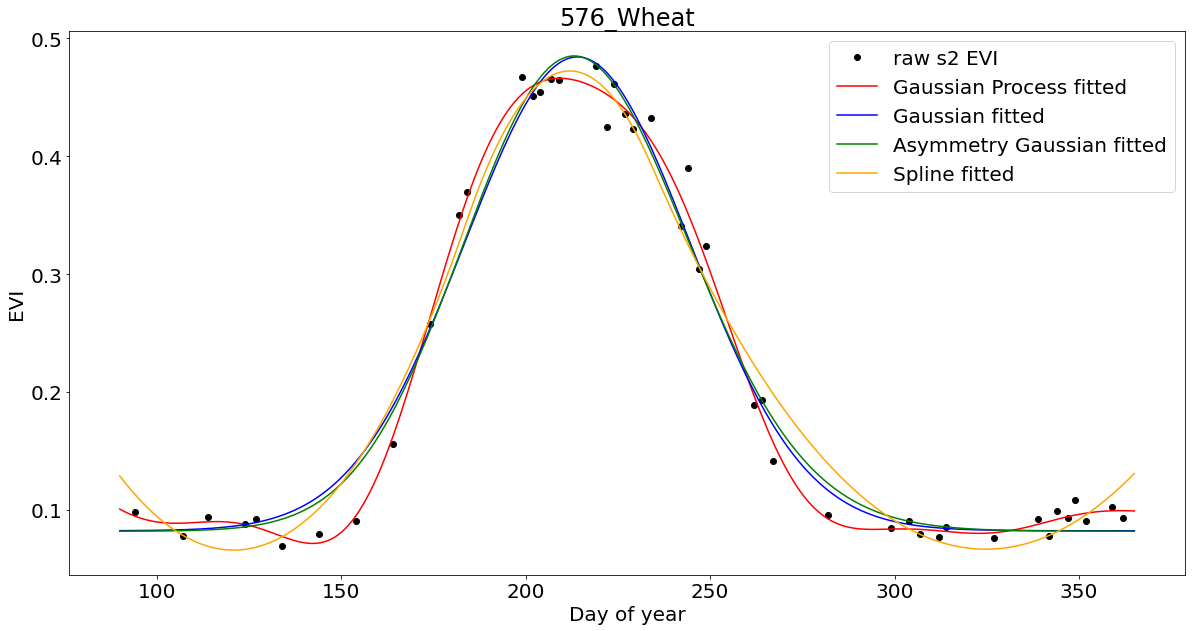
\includegraphics[scale=0.3]{img/yan_wheat_GPR_plot.png}
    \caption{Andries' team found that GPs where superior in terms of predicting a phenological timeline for a number of common seasonal crops over other parameteric models.}
    \label{fig: GP_motivate_wheat}
\end{figure}
Andries' team found that the only draw back to using GPs was the lengthy run time required to create predictions and fears that as more data is collected each season this would only exacerbate the issue. This is a common problem shared by anyone wanting to use GPs. Due to their unwieldy $\calO \left( n^3 \right)$ runtime, where $n$ is the number of observations,  GPs become impractical to apply on datasets with $n > 10^5$. The goal of this thesis is to explore various avenues one can take to replace some of the more intense calculations with computational more efficient approximations without sacrificing a great deal of precision.

Chapter \ref{Chapter1} will give a more mathematical treatment of GPs starting from the ground up by first giving a review of some essential material from functional analysis and then motivating the theory behind GPs before finally ending with a concrete algorithm for GP regression and classification. In chapter FIX and \ref{Chapter3} we shall look at techniques for approximating a large matrix that essentially provides information on how similar each observation is from one other. Chapter \ref{Chapter4} then gives alternative methods for solving linear systems which is an essential component required for GP algorithm to work.

\newpage
\addtocontents{toc}{\protect\setcounter{tocdepth}{2}}
%%%%%%%%%%%%%%%%%%%%%%%%%%%%%%%%%%%%%%%%%%%%%%%%%%%%%%%%%%%%%%%%%%%%%%%%%%%%%%%
\newpage

\section{Gaussian Processes}\label{Chapter1}
The aim of this chapter is to review some essential mathematical machinery required for us to understand the core concepts of Gaussian Processes.

\subsection*{Kernels}\label{Section1.1}

Often in machine learning we are often met with the challenge of how to best represent data instances as fixed size feature vectors $\bm{x}_i \in X$. For certain objects it might not be obvious at all how to represent the data as a fixed length vector. Good examples of variable length data include textual documents and genomic data. For these data types we can define a method of measuring similarity between objects which requires them to first be converted to a fixed length feature vector first \cite{MurphyKevinP2012Ml}. To do this we begin by mapping the feature vectors into a Hilbert space $\calH$ which enriches the vector space with an inner product $\langle \cdot , \cdot \rangle_{\calH} : \calH \times \calH \to \RR$ and a norm $\| \cdot \|_H : \calH \to \RR$. Input data is transformed into feature space vectors via a non-linear feature mapping $\Phi : X \to \calH$. The benefit of using feature maps in this way is that a non-linear descision boundary can be constructed using linear models. In some instances a similarity measure can be computed directly using a function $k : X \times X \to \RR$, instead of needing to construct a $\Phi$ and then computing the inner product of the transformed instances. Functions that act directly on our data instances are known as kernel functions and using them to avoid computation associated with the underlying feature space is known as the kernel trick \cite{SteinwartIngo2008SVMb}. These ideas are stated more formally in \Cref{defe: kernel}.

\begin{defe}[Kernel] \label{defe: kernel}
    Let $X$ be a non-empty set. Then a function $k : X \times X \to \RR$ is called a kernel on $X$ if there exists a Hilbert space and a map $\Phi : X \to \calH$ such that for all $\bm{x} , \bm{x}' \in X$ we have $k \left( \bm{x} , \bm{x}' \right) = \langle \Phi \left( \bm{x} \right), \Phi \left( \bm{x}' \right) \rangle_{\calH}$. We call the $\Phi$ the feature map and $\calH$ the feature space of $k$.
\end{defe}

It is worth noting that almost no conditions are placed on the set $X$, allowing it to accommodate virtually any form of data. It is not surprising then that neither the feature map nor the feature space are uniquely determined by the kernel. As shown by the example from Steinwart and Christmann \cite{SteinwartIngo2008SVMb}, when $X = \RR$ and $k \left( x , x' \right) = x \cdot x'$ where $x , x' \in X$, we can see that $k$ is a kernel using the feature map $\Phi \left( x \right) = x$ and $\calH = \RR$. However, another suitable feature map for this particular kernel is $\Phi' \left( x \right) = \left( x / \sqrt{2} , x / \sqrt{2} \right)$ with a corresponding feature space of $\calH = \RR^2$ since
\[
    \langle \Phi' \left( x \right), \Phi' \left( x' \right) \rangle_{\RR^2} = \frac{x'}{\sqrt{2}} \cdot \frac{x}{\sqrt{2}} + \frac{x'}{\sqrt{2}} \cdot \frac{x}{\sqrt{2}} = x \cdot x'
\]
for $x,x' \in X$. While their might be numerous functions that provide some notion of similarity between data entries, these functions might not be valid kernels. Instead of needing to construct a feature map and feature space to verify that a chosen function is a valid kernel using \Cref{defe: kernel}, we can make use of a much simpler set of criteria. Before embarking on this train of thought, we need to define the following.

\begin{defe}[Positive Definite and Positive Semidefinite] \label{defe: PD}
    A function $k : X \times X \to \RR$ is positive semidefinite if for all $n \in \NN$ and $\alpha_1 , \ldots , \alpha_n \in \RR$ and all $\bm{x}_1 ,\ldots , \bm{x}_n \in X$ we have
    \begin{equation}\label{eq: PSD}
        \sum_{i=1}^{n} \sum_{j=1}^{n} \alpha_i \alpha_j k \left( \bm{x}_j , \bm{x}_i \right) \geq 0.
    \end{equation}
    Furthermore, $k$ is said to be positive definite if for mutually distinct $\bm{x}_1 ,\ldots , \bm{x}_n \in X$ equality \Cref{eq: PSD} only holds for $\alpha_1 = \ldots = \alpha_n = 0$ \cite{SteinwartIngo2008SVMb}.
\end{defe}

\begin{defe}[Symmetric] \label{defe: Symmetric_function}
    A function $k : X \times X \to \RR$ is called symmetric if $k \left( \bm{x} , \bm{x}' \right) = k \left( \bm{x}' , \bm{x} \right)$ for any inputs $\bm{x}' , \bm{x} \in X$ \cite{SteinwartIngo2008SVMb}.
\end{defe}

\begin{defe}[Gram Matrix] \label{defe: Gram_Matrix}
    For fixed $\bm{x}_1 ,\ldots , \bm{x}_n \in X$ the matrix $\bm{K} \in \RR^{n \times n}$ where $\bm{K}_{i,j} \triangleq k \left( \bm{x}_j , \bm{x}_i \right)$ is the Gram matrix \cite{SteinwartIngo2008SVMb}.
\end{defe}

Note that checking if a function is positive (semi) definite is equivalent to checking that any Gram matrix produced by a function is positive (semi) definite. If $k$ is a real valued kernel corresponding to the feature map $\Phi$, then $k$ is symmertic by virtue of the fact that the inner product of a real Hilbert space is symmetric. Moreover $k$ is positive definite since for $\alpha_1 , \ldots , \alpha_n \in \RR$ and $\bm{x}_1 ,\ldots , \bm{x}_n \in X$ we have
\begin{align*}
     & \sum_{i=1}^{n} \sum_{j=1}^{n} \alpha_i \alpha_j k \left( \bm{x}_j , \bm{x}_i \right)                                                 \\
     & = \sum_{i=1}^{n} \sum_{j=1}^{n} \alpha_i \alpha_j \langle \Phi \left( \bm{x}_i \right), \Phi \left( \bm{x}_j \right) \rangle_{\calH} \\
     & = \norm{ \sum_i^n \alpha_i \Phi \left( \bm{x}_i \right) }_{\calH}^{2}                                                                \\
     & \geq 0.
\end{align*}

The following theorems tell us that it is not only necessary for a kernel to be positive semi definite but it is also a sufficient condition.

\begin{thm} \label{theorem: nec_and_suf_kernel_1}
    A function $k : X \times X \to \RR$ is a kernel if and only if it is symmertic and positive semidefinite \cite{SteinwartIngo2008SVMb}*{page 118}.
\end{thm}

\begin{proof}
    In view of the above discussion, it suffices to show that a symmetric and positive definite function is a kernel. To this end, we write
    \begin{equation*}
        \calH_{\text{pre}} \triangleq \left\{ \sum_{i=1}^{n} \alpha_{i} k (\cdot , \bm{x}_{i}) \mid n \in \NN , \; \alpha_1 , \ldots , \alpha_n \in \RR , \; \bm{x}_{1} , \ldots , \bm{x}_{n} \in X \right\}
    \end{equation*}
    and for $f \triangleq \sum_{i=1}^{n} \alpha_{i} k (\cdot , \bm{x}_{i}) \in \calH_{\text{pre}}$ and $g \triangleq \sum_{j=1}^{m} \beta_{j} k (\cdot , \bm{x}_{j}') \in \calH_{\text{pre}}$, we define
    \begin{equation*}
        \langle f,g \rangle \triangleq \sum_{i=1}^{n} \sum_{j=1}^{m} \alpha_{i} \beta_{j} k (\bm{x}_{j}' , \bm{x}_{i}).
    \end{equation*}
    Note that this definition is independent of the representation of $f$ since we have $\langle f,g \rangle = \sum_{j=1}^{m} \beta_{i}  f (\bm{x}_{j}')$. Furthermore, by the symmetry of $k$, we find $\langle f,g \rangle = \sum_{i=1}^{m} \alpha_{i}  g (\bm{x}_{i})$, that is, the definition is also independent of the representation of $g$. Moreover, the definition immediately shows that $\langle \cdot , \cdot \rangle$ is bilinear and symmeteric, and since $k$ is positive definite, $\langle \cdot , \cdot \rangle$ is also positive, that is, $\langle f , f \rangle \geq 0$ for all $f \in \calH_{\text{pre}}$. Consequently, $\langle \cdot , \cdot \rangle$ satisfies the Cauchy-Schwarz inequality, that is,
    \begin{equation*}
        \left| \langle f,g \rangle \right|^2 \leq \langle f , f \rangle \cdot \langle g , g \rangle, \quad f,g \in \calH_{\text{pre}}.
    \end{equation*}
    Now let $f \triangleq \sum_{i=1}^{n} \alpha_{i} k (\cdot , \bm{x}_{i})$ with $\langle f , f \rangle = 0$. Then for all $\bm{x} \in X$, we have
    \begin{equation*}
        \left| f(\bm{x}) \right|^2 = \left| \sum_{i=1}^{n} \alpha_i k (\bm{x} , \bm{x}_i) \right|^2 = \left| \langle f , k (\cdot , \bm{x}) \rangle \right|^2 \leq  \langle k (\cdot , \bm{x}) , k (\cdot , \bm{x}) \rangle \cdot \langle f , f \rangle
    \end{equation*}
    and hence we find that $f = \bm{0}$. Therefore we have shown that $\langle \cdot , \cdot \rangle$ is an inner product on $\calH_{\text{pre}}$. Let $\calH$ be a completion of $\calH_{\text{pre}}$ and $I : \calH_{\text{pre}} \to \calH$ be the corresponding isometeric embedding. Then $\calH$ is a Hilbert space and we have
    \begin{equation*}
        \langle I k (\cdot , \bm{x}') , I k (\cdot , \bm{x}) \rangle_{\calH} = \langle k (\cdot , \bm{x}') , k (\cdot , \bm{x}) \rangle_{\calH_{\text{pre}}} = k (\bm{x} , \bm{x}')
    \end{equation*}
    for all $\bm{x} , \bm{x}'$, that is, $\bm{x} \mapsto I k (\cdot , \bm{x}), \; \bm{x} \in X$, defines a feature map of $k$.
\end{proof}

\subsection{Reproducing Kernel Hilbert Spaces}\label{Section1.2}

We shall now shift our attention towards reproducing kernel Hilbert spaces (RKHS) and describe their relation to kernels. We shall see that in some sense the RKHS of a kernel $k$ is the smallest feature space for a kernel. The formal definition of a RKHS is stated in definition \ref{defe: RKHS}.

\begin{defe}[RKHS] \label{defe: RKHS}
    Let $X \neq \emptyset$ and $H$ be a real Hilbert space over $X$
    \begin{enumerate}
        \item A function $k : X \times X \to \RR$ is called a reproducing kernel if we have $k \left( \cdot, \bm{x} \right) \in H$ for all $\bm{x} \in X$ and the reproducing property
              \[
                  f(\bm{x}) = \langle f , k \left( \cdot, \bm{x} \right) \rangle
              \]
              holds for all $f \in H$ and $x \in X$.
        \item The space $H$ is called a reproducing kernel Hilbert space over $X$ if for all $\bm{x} \in X$ the Dirac functional $\delta_{\bm{x}} : H \to \RR$ defined by $\delta_{\bm{x}} (f) \triangleq f(x), \; f \in H$ is continuous.
    \end{enumerate}
    \cite{SteinwartIngo2008SVMb}
\end{defe}

An important property of the RKHS is that the convergence in the norm implies pointwise convergence. Specifically in a RKHS for any sequence of functions $\left\{ f_n \right\} \subset H$ where $\norm{f_n - f} \to 0$ we have $\abs{\delta_{\bm{x}} (f_n) - \delta_{\bm{x}} (f)} = \abs{f_n (x) - f (x)} \to 0$. Note that because the evaluation function is both linear and continuous then it is also bounded in the sense that there is an $c \in \RR, \; c > 0$ such that for every $f \in H$ and a fixed $\bm{x} \in X$ we have $\abs{\delta_{\bm{x}} (f)} \leq c \norm{f}_H$ \cite{BerezanskyMakarovich1996FaV1}. This property of uniform convergence implying pointwise convergence is important since it tells us that if functions $f,g \in H$ are close in norm then their evaluation at any point is also similar. The following lemma ties together the definition of an RKHS, reproducing kernel and a kernel.

\begin{lem}[] \label{lem: RKHS_rk_k}
    Let $H$ be a Hilbert function space over $X$ that has a reproducing kernel $k$. Then $H$ is a RKHS and $H$ is also a feature space of $k$ where the feature map $\Phi : X \to H$ is given by
    \[
        \Phi (\bm{x}) = k \left( \cdot , \bm{x}  \right)
    \]
    for some $\bm{x} \in X$. We call $\Phi$ the canonical feature map.
\end{lem}

\begin{proof}
    Since the reproducing property tells us that any Dirac functional can be represented by the reproducing kernel this means
    \[
        \abs{\delta_{\bm{x}} (f)} = \abs{f(\bm{x})} = \abs{\langle f , k \left( \cdot, \bm{x} \right) \rangle} \leq \norm{k \left( \cdot, \bm{x} \right)}_H \cdot \norm{f}_H
    \]
    for all $\bm{x} \in X, \; f \in H$. This shows continuity of $\delta_{\bm{x}}$ for $\bm{x} \in X$. In order to show that $\Phi$ is a feature map, fix an $\bm{x}' \in X$ and set $f = k \left( \cdot, \bm{x}' \right)$. Then for $\bm{x} \in X$, the reproducing property yields
    \[
        \langle \Phi (\bm{x}') , \Phi (\bm{x}) \rangle_H = \langle k \left( \cdot, \bm{x}' \right) , k \left( \cdot, \bm{x} \right) \rangle_H = \langle f , k \left( \cdot, \bm{x} \right) \rangle_H = f(\bm{x}) = k \left( \bm{x}', \bm{x} \right).
    \]
\end{proof}

This tells us that every Hilbert space with a reproducing kernel is a RKHS. We can also show the converse, that is, every RKHS has a unique reproducing kernel seen in theorem \ref{theorem: unique_kernel}.

\begin{thm} \label{theorem: unique_kernel}
    Let $H$ be a RKHS over $X$. Then $k: X \times X \to \RR$ defined by $k \left( \bm{x}', \bm{x} \right) = \langle \delta_{\bm{x}} , \delta_{\bm{x}'} \rangle_H, \; \bm{x} , \bm{x}' \in X$ is the only reproducing kernel of $H$ \cite{SteinwartIngo2008SVMb}.
\end{thm}

Theorem \ref{theorem: unique_kernel} shows that a RKHS is uniquely determined by its kernel. In fact the other direction can also be shown giving a one-to-one correspondence between kernels and RKHS. This is known as the Moore-Aronszajn theorem presented in thorem \ref{theorem: Moore-Aronszajn}.

\begin{thm}[Moore-Aronszajn] \label{theorem: Moore-Aronszajn}
    Suppose $k$ is a symmertic positive definite kernel on a set $X$. Then there is a unique Hilbert space of functions for which $k$ is the reproducing kernel \cite{BerlinetAlain2003RKHS}.
\end{thm}

The elements of a RKHS will often inherit the analytical properties of its corresponding kernel. This means that kernels provide a mechanism for generating spaces of functions with useful analytical properties.

\subsection{Gaussian Radial Basis Kernel}\label{Section1.3}

We shall now focus on a specific class of kernel that shall be used extensively in upcoming theory and experimentation.

\begin{defe}[Gaussian Radial Basis Kernel] \label{defe: grbfk}
    For $d \in \NN, \; \sigma > 0, \; \bm{z} , \bm{z}' \in \RR^d$ we define
    \[
        k_\sigma \left( \bm{z} , \bm{z}' \right) \triangleq \exp \left( - \sigma^{-2} \sum_{j=1}^{d} \left( \bm{z}_j - {\bm{z}'}_j \right)^2 \right).
    \]
    Then $k_\sigma$ is a real valued kernel called the Gaussian Radial Basis Kernel (RBF) kernel with bandwidth $\sigma$. Moreover $k_\sigma$ can be computed as
    \[
        \exp \left( \frac{- \norm{\bm{z} - {\bm{z}'}}_{2}^{2}}{\sigma^2} \right)
    \]
    \cite{SteinwartIngo2008SVMb}.
\end{defe}
The Gaussian RBF kernel makes for a very simple an intuitive measurement of similarity between its inputs. One geometric interpretation of the Gaussian RBF kernel is that as the radius of the smallest $d$-sphere containing $\bm{z} , \bm{z}' \in \RR^d$ grows the corresponding measurement of similarity decays exponentially. A visual representation of this decay is shown in figure \ref{fig: grbfk_graph_1}.

\begin{figure}[H]
    \centering
    \subfloat{
        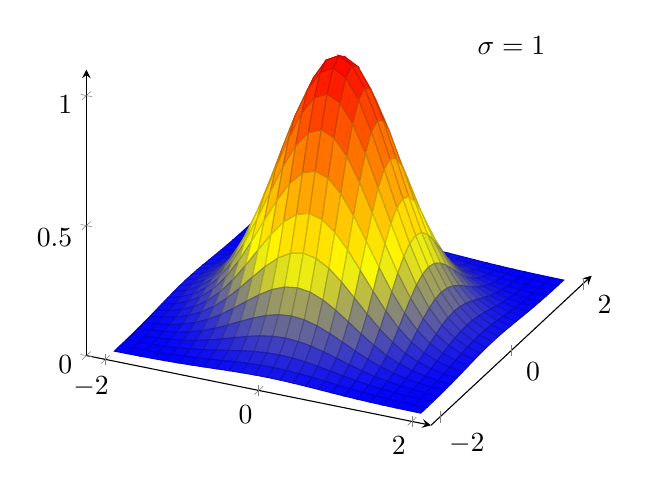
\begin{tikzpicture}

            \begin{axis}[
                    width=8cm,height=8cm,
                    domain=-2:2,
                    xmax=2.25,
                    ymax=2.25,
                    xmin=-2.25,
                    ymin=-2.25,
                    zmax=1.1,
                    axis lines = left,
                    colormap/hot,
                ]

                \addplot3[samples = 25, surf] {exp(-(x^2 + y^2)/1)};
                \node at (rel axis cs:1,0.5,1) [above] {\(\sigma=1\)};

            \end{axis}

        \end{tikzpicture}
    }%
    \quad
    \subfloat{
        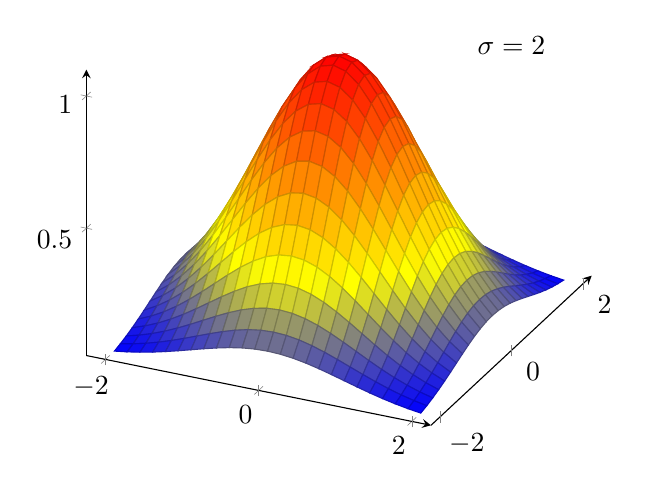
\begin{tikzpicture}

            \begin{axis}[
                    width=8cm,height=8cm,
                    domain=-2:2,
                    xmax=2.25,
                    ymax=2.25,
                    xmin=-2.25,
                    ymin=-2.25,
                    zmax=1.1,
                    axis lines = left,
                    colormap/hot,
                ]

                \addplot3[samples = 25, surf] {exp(-(x^2 + y^2)/2)};
                \node at (rel axis cs:1,0.5,1) [above] {\(\sigma=2\)};

            \end{axis}

        \end{tikzpicture}
    }%
    \caption{A graph of the Gaussian RBF from definition \ref{defe: grbfk} for $d=2$. Evidently, a larger value of $\sigma$ slows the rate of decay increasing the similarity between the same pair of samples.}%
    \label{fig: grbfk_graph_1}
\end{figure}

This kernel is infinitely differentiable meaning it has mean square derivatives of all orders and is therefore very smooth. In fact, some argue that such strong smoothness makes it unrealistic for modelling natural phenomena \cite{RasmussenCarlEdward2006Gpfm,SteinMichaelL1999IoSD}. Nontheless, Gaussian RBF kernelis still the one of the most widely used kernels in literature.

\subsection{Kernel Machines}\label{Section1.4}

In this section, we shall look at two different machine learning models that make use of kernels to perform classification and regression. The first kernel machine we shall look at are support vector machines (SVM). SVMs where originally designed for binary classification and as such we shall only present a model for binary classification, although extensions exist that allow regression and multi-class classification.

For the binary classification problem we are tasked with labelling new samples with either one of two classes, $-1$ or $1$. We shall assume our input space consists of vectors from $\RR^d$ and that we provided with a labelled training set $D = \left\{ \left( \bm{x}_1 , y_1 \right), \left( \bm{x}_1 , y_1 \right), \ldots , \left( \bm{x}_n , y_n \right) \right\}$. One simple method to classify samples is by creating an affine linear hyperplane satisfying
\begin{align} \label{eq: linear_sep_hyp}
    \langle \bm{w}, \bm{x}_i \rangle + b > 0, \quad y_i = +1 \nonumber \\
    \langle \bm{w}, \bm{x}_i \rangle + b < 0, \quad y_i = -1
\end{align}
for some $\bm{w} \in \RR^d$ and $b \in \RR$ where $\norm{w}_2 = 1$. Moreover we would like $\bm{w}$ and $b$ to maximise the margin, that is the maximal distance between the separating hyperplane and the points in $D$. The specific $\bm{w}$ and $b$ obtained through the training set is denoted $\bm{w}_D$ and $b_D$ and the resulting descision function is defined as
\[
    f_D \left( \bm{x} \right) \triangleq \operatorname{sign} \left( \langle \bm{w}_D , \bm{x} \rangle + b_D \right).
\]
There are, however, a number of short comings to this model. The most obvious is that our training data may not be linearly separable in $\RR^d$ meaning that no such $\bm{w}_D$ and $b_D$ exist. Moreover, when noise is introduced to the data set this model will prioritize finding a hyperplane that perfectly separates the two classes, making no comprises in misclassifying points, leaving it subject to overfitting. SVMs where introduced by Boser {\it et al.} \cite{BoserBernhard1992Ataf} to address the first issue of separability. Their approach was to lift the input vector into a more malleable Hilbert space $H_0$ using a feature map. The inputs are then classified within the new space. Unfortunately this method does nothing to address the second issue of over fitting and, if anything, actually worsens it. Cortes and Vapnik \cite{CortesCorinna1995SN} attempted to address this second issue by introducing slack variables to equation \ref{eq: linear_sep_hyp} so that we instead need to satisfy $y_i \left( \langle \bm{w} , \Phi \left( \bm{x}_i \right) \rangle + b \right) \geq 1 - \xi_i$ for some $\xi_i \in \RR_{>0}$. These constraints can be re-written as
\[
    \xi_i \geq 1 - y_i \left( \langle \bm{w} , \Phi \left( \bm{x}_i \right) \rangle + b \right)
\]
and combining this this our slack constraints (that is $\xi_i \geq 0$) yields
\[
    \xi_i \geq \max \left\{ 0, 1 - y_i \left( \langle \bm{w} , \Phi \left( \bm{x}_i \right) \rangle + b \right)  \right\} = L_{\text{hinge}} \left( y_i , \langle \bm{w} , \Phi \left( \bm{x}_i \right) \rangle + b \right)
\]
where $L_{\text{hinge}}$ is the hinge loss defined as
\[
    L_{\text{hinge}} \left( y,\eta \right) \triangleq \max \left\{ 0,1-y\eta \right\}.
\]
This optimization problem can be re-written is the form
\[
    \min_{\left( \bm{w} , b \right) \in H_0 \times \RR} \lambda \norm{\bm{w}}_{H_0} + \frac{1}{n} \sum_{i=1}^{n} L_{\text{hinge}} \left( y_i , f_{\left( \bm{w} , b \right)} \right)
\]
where $f_{\left( \bm{w} , b \right)} : X \to \RR$ is defined as
\[
    f_{\left( \bm{w} , b \right)} \triangleq \langle \bm{w} , \Phi \left( x_i \right) \rangle + b.
\]
Unfortunately, this new embedding requires us to solve for optimal parameters in a very high, or even infinite, dimension vector space. To get around this, often the Lagrange approach is used to solve the corresponding dual problem. When the hinge loss is used the dual problem becomes
\begin{align} \label{eq: SVM_dual_1}
     & \max_{\alpha \in \left[ 0,C \right]^n} \sum_{i=1}^{n} \alpha_i - \frac{1}{2} \sum_{i,j=1}^{n} y_i y_j \alpha_i \alpha_j \langle \Phi \left( \bm{x}_i \right), \Phi \left( \bm{x}_j \right) \rangle \nonumber \\
     & \text{subject to} \quad \sum_{i=1}^{n} y_i \alpha_i = 0
\end{align}
Notice that in the dual problem, we find that inner products are only taken with vectors that have the feature map applied to them allowing us to employ the kernel if the corresponding kernel trick described in section \ref{Section1.1} is known for the feature map used so that \ref{eq: SVM_dual_1} becomes
\begin{align*}
     & \max_{\alpha \in \left[ 0,C \right]^n} \sum_{i=1}^{n} \alpha_i - \frac{1}{2} \sum_{i,j=1}^{n} y_i y_j \alpha_i \alpha_j k \left( \bm{x}_i, \bm{x}_j \right) \\
     & \text{subject to} \quad \sum_{i=1}^{n} y_i \alpha_i = 0.
\end{align*}

The next machine learning model of interest that uses kernels are gaussian processes. To motivate this model, consider the time series data in figure \ref{fig: motive_gp_1}.

\begin{figure}[H]
    \centering
    \subfloat[]{
        \begin{tikzpicture}
            \draw[->,thick] (-0.01,0)--(6,0) node[right]{$x$};
            \draw[->,thick] (0,-0.01)--(0,6) node[above]{$y$};

            \draw[-,ultra thick] (0.7,-0.1)--(0.7,0.1) node[below,yshift=-0.3cm]{$x_1$};
            \draw[fill,draw,blue] (0.7,0.5) circle[radius=2.5pt];

            \draw[-,ultra thick] (1.4,-0.1)--(1.4,0.1) node[below,yshift=-0.3cm]{$x_2$};
            \draw[fill,draw,blue] (1.4,0.6) circle[radius=2.5pt];

            \draw[-,ultra thick] (2.7,-0.1)--(2.7,0.1) node[below,yshift=-0.3cm]{$x_3$};
            \draw[fill,draw,blue] (2.7,1.7) circle[radius=2.5pt];

            \draw[-,ultra thick] (3.7,-0.1)--(3.7,0.1) node[below,yshift=-0.2cm]{$x^{\ast}$};
            \draw[dashed,thick,red] (3.7,0)--(3.7,5);

            \draw[-,ultra thick] (5,-0.1)--(5,0.1) node[below,yshift=-0.3cm]{$x_4$};
            \draw[fill,draw,blue] (5,4) circle[radius=2.5pt];
        \end{tikzpicture}
    }%
    \qquad
    \subfloat[]{
        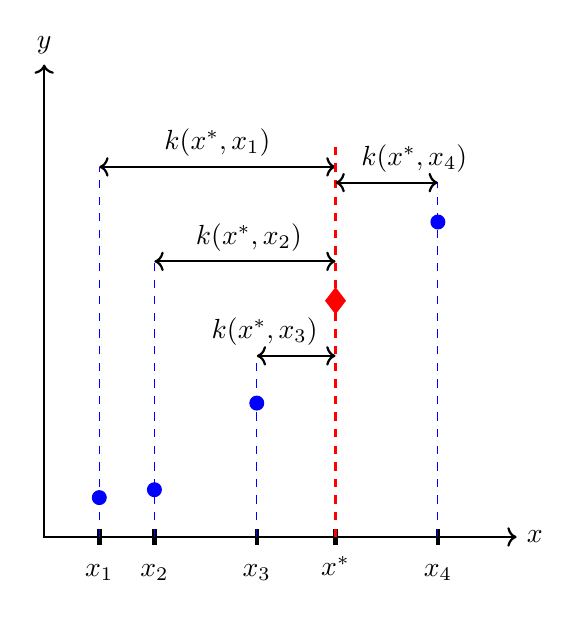
\begin{tikzpicture}
            \draw[->,thick] (-0.01,0)--(6,0) node[right]{$x$};
            \draw[->,thick] (0,-0.01)--(0,6) node[above]{$y$};

            \draw[-,ultra thick] (0.7,-0.1)--(0.7,0.1) node[below,yshift=-0.3cm]{$x_1$};
            \draw[fill,draw,blue] (0.7,0.5) circle[radius=2.5pt];
            \draw[dashed,blue] (0.7,0)--(0.7,4.7);
            \draw[<->,thick] (0.7,4.7)--(3.7,4.7) node[above,xshift=-1.5cm]{$k(x^{\ast},x_1)$};

            \draw[-,ultra thick] (1.4,-0.1)--(1.4,0.1) node[below,yshift=-0.3cm]{$x_2$};
            \draw[fill,draw,blue] (1.4,0.6) circle[radius=2.5pt];
            \draw[dashed,blue] (1.4,0)--(1.4,3.5);
            \draw[<->,thick] (1.4,3.5)--(3.7,3.5) node[above,xshift=-1.1cm]{$k(x^{\ast},x_2)$};

            \draw[-,ultra thick] (2.7,-0.1)--(2.7,0.1) node[below,yshift=-0.3cm]{$x_3$};
            \draw[fill,draw,blue] (2.7,1.7) circle[radius=2.5pt];
            \draw[dashed,blue] (2.7,0)--(2.7,2.3);
            \draw[<->,thick] (2.7,2.3)--(3.7,2.3) node[above,xshift=-0.9cm]{$k(x^{\ast},x_3)$};

            \draw[-,ultra thick] (3.7,-0.1)--(3.7,0.1) node[below,yshift=-0.2cm]{$x^{\ast}$};
            \node[diamond,draw,fill,draw,red,minimum width = 1cm,minimum height = 1.3cm,scale=0.25] (d) at (3.7,3) {};
            \draw[dashed,thick,red] (3.7,0)--(3.7,5);

            \draw[-,ultra thick] (5,-0.1 )--(5,0.1) node[below,yshift=-0.3cm]{$x_4$};
            \draw[fill,draw,blue] (5,4) circle[radius=2.5pt];
            \draw[dashed,blue] (5,0)--(5,4.5);
            \draw[<->,thick] (3.7,4.5)--(5,4.5) node[above,xshift=-0.3cm]{$k(x^{\ast},x_4)$};
        \end{tikzpicture}
    }%
    \caption{A graph of the Gaussian RBF from definition \ref{defe: grbfk} for $d=2$. Evidently, a larger value of $\sigma$ slows the rate of decay increasing the similarity between the same pair of samples.}%
    \label{fig: motive_gp_1}
\end{figure}

\begin{filecontents*}{./data/gp_intro_dat1.csv}
    x,y0,y1,y2
    0.0,3.8889447299776054,3.252195675396163,2.5723986201044187
    0.10204081632653061,3.8963153731866624,3.2334114175675395,2.4977761527857716
    0.20408163265306123,3.904676475191245,3.2263277175862597,2.4161726074738854
    0.30612244897959184,3.912486422260641,3.2265022294195966,2.3292200441690207
    0.40816326530612246,3.9181367775658873,3.228192583362307,2.2398507798591534
    0.5102040816326531,3.920256370846241,3.2249223304542913,2.152200525625582
    0.6122448979591837,3.9179701155023157,3.2101098230475538,2.071344891386562
    0.7142857142857143,3.9110778971645765,3.1777033459669783,2.0028774256062816
    0.8163265306122449,3.9001283490397016,3.122766415820061,1.9523672809629247
    0.9183673469387755,3.886376053031046,3.04196343041673,1.924753149634383
    1.0204081632653061,3.8716211994498333,2.933909038317024,1.9237443590136485
    1.1224489795918369,3.857954079608229,2.799351626306004,1.9513035606887854
    1.2244897959183674,3.847436905468257,2.6411768356723235,2.0072815139900495
    1.3265306122448979,3.841775787363871,2.4642319083119633,2.0892569830605368
    1.4285714285714286,3.8420321968485376,2.2749858593824617,2.192613833596985
    1.5306122448979593,3.8484268708760094,2.081057401633018,2.310856060666622
    1.6326530612244898,3.8602681088894766,1.8906546442626817,2.436135561712868
    1.7346938775510203,3.876016440194414,1.7119803587951616,2.559934911031695
    1.836734693877551,3.8934729250514666,1.5526570590488398,2.6738332705910244
    1.9387755102040818,3.9100510027824393,1.4192260798320049,2.7702684624537106
    2.0408163265306123,3.9230775813589482,1.3167595333633981,2.8432111425013322
    2.142857142857143,3.9300643637480857,1.248613256762677,2.888679554257369
    2.2448979591836737,3.9289011237509577,1.2163272198562576,2.905046033347129
    2.3469387755102042,3.9179401795449396,1.2196699093041794,2.8931101011392846
    2.4489795918367347,3.8959727008352174,1.2568027645405968,2.855945899531336
    2.5510204081632653,3.8621237371394623,1.3245411459916354,2.7985513820415195
    2.6530612244897958,3.8157151558884888,1.418678279406553,2.7273502460278247
    2.7551020408163267,3.756152285749804,1.5343452363886438,2.6496002463865618
    2.857142857142857,3.682888390340987,1.6663820121189532,2.5727700517645653
    2.9591836734693877,3.595495808498078,1.809697591321269,2.5039341546455005
    3.0612244897959187,3.493850568209357,1.9596010720146781,2.449232028447514
    3.163265306122449,3.378399275439287,2.1120883798539003,2.413420573364779
    3.2653061224489797,3.250456289718835,2.2640650594565668,2.3995428209525658
    3.36734693877551,3.1124629519607803,2.4134903440220477,2.4087275907808734
    3.4693877551020407,2.968139731618476,2.559424609970991,2.4401239977854456
    3.5714285714285716,2.8224826195273596,2.701970562220883,2.4909781807485927
    3.673469387755102,2.6815760504255355,2.8421022219924184,2.556846086350459
    3.7755102040816326,2.5522348648343,2.9813911671556212,2.6319349647504673
    3.8775510204081636,2.441513722741859,3.1216501445256846,2.709555194481732
    3.979591836734694,2.3561485591504203,3.264528290179406,2.7826529438164505
    4.081632653061225,2.3020051023456194,3.4111042700896737,2.8443841134520453
    4.183673469387755,2.2836063990304716,3.5615279847182504,2.8886791623908876
    4.285714285714286,2.3037932704691393,3.7147625310871684,2.9107453218748542
    4.387755102040816,2.3635503438936984,3.8684692167316403,2.907454656505577
    4.4897959183673475,2.461999004872191,4.019063544907245,2.8775731008424583
    4.591836734693878,2.596536742969357,4.161947681776214,2.821805978895311
    4.6938775510204085,2.763082806314141,4.291903941920607,2.742656025464969
    4.795918367346939,2.9563825813547977,4.4036048056748225,2.644116725967176
    4.8979591836734695,3.1703270754187236,4.492179720561176,2.5312380314160974
    5.0,3.398251248127017,4.553760976976619,2.4096316234579827
\end{filecontents*}

\begin{tikzpicture}
    \begin{axis}[
            xmin=-0.0,xmax=6.5,
            ymin=-0.5,ymax=6.5,
            axis line style={draw=none},
            tick style={draw=none},
            yticklabels=\empty,
            xticklabels=\empty,
        ]
        \addplot[smooth, color=black, semithick] table [x=x, y=y0, col sep=comma, mark=none] {./data/gp_intro_dat1.csv};
        \addplot[smooth, color=black, semithick, dashed] table [x=x, y=y1, col sep=comma, mark=none] {./data/gp_intro_dat1.csv};
        \addplot[smooth, color=black, semithick, dotted] table [x=x, y=y2, col sep=comma, mark=none] {./data/gp_intro_dat1.csv};
    \end{axis}
    \draw[->,thick] (0,0.5)--(0,5.5) node[above]{$y$};
    \draw[->,thick] (0,0.5)--(6,0.5) node[right]{$x$};
\end{tikzpicture}


\subsection{Gaussian Processes for Regression}\label{Section1.5}

We saw in section \ref{Section1.4} that, unlike most other machine learning models, GPs infer over a distribution of functions $p \left( f \mid D \right)$ instead of a vector of parameteric values $p \left( \bm{\theta} \mid D \right)$. Naively, one may attempt to find a suitable $f$ by fixing a class of functions $\calF$ and then search over this class to find a function that best represents the data. However, this may not work well if there is not enough richness in $\calF$ to represent the data. Instead we choose a suitable $f$ by assigning a prior probability to every possible function using the training data and then to select the function with the highest probability. To keep this computation tractable we only evalute our predicted function at a finite number of points. The prediction itself is found by taking the mean over all functions with respect to the posterior conditioned on the observed data which is assumed to be jointly Gaussian with the input value. This gives rise to Gaussian Process more formally stated in definition \ref{defe: GP}.

\begin{defe}[Gaussian Process] \label{defe: GP}
    A Gaussian Process (GP) is a collection of random variables with index set $I$, such that every finite subset of random variables has a joint Gaussian distribution \cite{RasmussenCarlEdward2006Gpfm,MurphyKevinP2012Ml}.
\end{defe}

A GP is completely characterised by a mean function $m(\bm{x})$ and a kernel, which in the context of GPs is sometimes called a covariance function, $k (\bm{x}, \bm{x'})$ on a real process as
\begin{align*}
    m(\bm{x})           & = \EE \left[ f(\bm{x}) \right]                                         \\
    k (\bm{x}, \bm{x'}) & = \EE \left[ (f(\bm{x}) - m(\bm{x})) (f(\bm{x'}) - m(\bm{x'})) \right]
\end{align*}
GPs define a prior over all possible functions which can be used to create a posterior once enough data has been observed. The prior is used to represent the functions we expect to see before any observations are made. Although defining a prior over all possible function may seem computationally intractable, we actually only need to define a distribution over a finite number of points. Before any observations are made, we typically assume that the mean function is the constant zero function, that is $m \left( \bm{x} \right) = 0$. A function $f(\bm{x})$ sampled from a GP with mean $m(\bm{x})$ and covariance $k (\bm{x}, \bm{x'})$ is written as
\[
    f(\bm{x}) \sim \calG \calP \left( m(\bm{x}), k (\bm{x}, \bm{x'}) \right)
\]
Since a GP is a collection of random variables it must satisfy the consistency requirement, that is, an observation of a set of variables should not the distribution of any small sub set of the observed values. More specifically if
\[
    (\bm{y_1}, \bm{y_2}) \sim \calN (\bm{\mu}, \bm{\Sigma})
\]
then
\begin{align*}
    \bm{y_1} & \sim \calN (\bm{\mu_1}, \bm{\Sigma_{1,1}}) \\
    \bm{y_2} & \sim \calN (\bm{\mu_2}, \bm{\Sigma_{2,2}})
\end{align*}

where $\bm{\Sigma_{1,1}}$ and $\bm{\Sigma_{2,2}}$ are the relevant sub matrices. Again, we shall us the notation that for set of data $\bm{W} = \left[ \bm{w}_1 ,\bm{w}_2 , \ldots , \bm{w}_n \right]^{\intercal} \in \RR^{n \times d}$ and $\bm{W}' = \left[ \bm{w}_1' ,\bm{w}_2' , \ldots , \bm{w}_m' \right]^{\intercal} \in \RR^{n' \times d}$ we use the notation
\[
    \left( \bm{K}_{\bm{W} \bm{W}'} \right)_{i,j} \triangleq k \left( \bm{w}_i , \bm{w}_j' \right)
\]
where \( \bm{K}_{\bm{W} \bm{W}'} \in \RR^{n \times n'} \). The convariance function completely characterized by its kernel. Unless otherwise stated, the kernel or covariance function used in examples and experimentation in the Gaussian RBF kernel, definition \ref{defe: grbfk}. To understand this better, as a small exercise we can select a number of inputs $\bm{X}^{\star} = \left[ \bm{x}_1 , \bm{x}_2 , \ldots , \bm{x}_{n^{\star}} \right]^{\intercal} \in \RR^{n^{\star} \times d}$ of compute the corresponding covariance matrix using the Gaussian RBF kernel. Gaussian vectors can then be sampled using a joint Gaussian distribution using the covariance matrix from the distribution
\[
    \bm{f}^{\star} \sim \calN \left( \bm{0}, \bm{K_{X^{\star} X^{\star}}} \right)
\]
graph its values as a function of its inputs.

\begin{filecontents*}{./data/gp_intro_dat1.csv}
    x,y0,y1,y2
    0.0,2.6341780930873786,4.41685044685407,1.884123117075101
    0.11224489795918367,2.685150340856032,4.351109330694541,2.0933788453347146
    0.22448979591836735,2.758222906849677,4.246986054733594,2.3215583495507697
    0.336734693877551,2.844091796198551,4.111722477611423,2.5621308980348045
    0.4489795918367347,2.9327004798948444,3.954138391914307,2.8093607381581323
    0.5612244897959183,3.0142490315111,3.7837568463624893,3.058296829896802
    0.673469387755102,3.0800293333419133,3.609905398833131,3.304575221937234
    0.7857142857142857,3.1230071846450134,3.4408573216000065,3.5440886761610075
    0.8979591836734694,3.1381275068842287,3.2830844115325393,3.772606115615495
    1.010204081632653,3.1223796951701805,3.1407028040204787,3.985434762859824
    1.1224489795918366,3.074690487867501,3.0151840031490704,4.177213384641246
    1.2346938775510203,2.99572649694323,2.9053883056890326,4.341906534238328
    1.346938775510204,2.887680093346262,2.807934404050683,4.473021654529128
    1.4591836734693877,2.7540712359611135,2.7178753181761683,4.5640359352552755
    1.5714285714285714,2.5995639802641644,2.629596908378246,4.608968085491204
    1.683673469387755,2.4297636797240854,2.537815790076743,4.603008456947798
    1.7959183673469388,2.250945266539242,2.4385306514757277,4.54310273176884
    1.9081632653061225,2.0696826217289814,2.3297825969976156,4.428402138611055
    2.020408163265306,1.8923794707563157,2.2121155584786374,4.26051300065903
    2.13265306122449,1.724750314129252,2.088670901030661,4.043522033936433
    2.2448979591836733,1.5713409480295042,1.9649185604698398,3.78380984825793
    2.357142857142857,1.4351902937232137,1.8480772970914263,3.4896953544368947
    2.4693877551020407,1.3177316537250037,1.7463209648090843,3.170973707657322
    2.5816326530612246,1.2189781885886188,1.667887909534986,2.838411584600058
    2.693877551020408,1.137982180009872,1.6202034591848866,2.503253609595508
    2.806122448979592,1.0734814750833834,1.6091067041507867,2.176777775544475
    2.9183673469387754,1.0246008560812094,1.638242628202587,1.8699164299237567
    3.0306122448979593,0.9914469543413351,1.708653796550625,1.5929463528940093
    3.142857142857143,0.9754532832118712,1.8185871450769515,1.3552308689036683
    3.2551020408163267,0.9793831046385866,1.9635250522558478,1.1649988273056024
    3.36734693877551,1.0069633897912214,2.136445411268843,1.0291341361289352
    3.479591836734694,1.0622134340832736,2.328310102622806,0.9529576266820667
    3.5918367346938775,1.1485904962060034,2.5287676666005745,0.9399816624503701
    3.704081632653061,1.2681182060719118,2.7270230125223396,0.9916380696381344
    3.816326530612245,1.4206777569266578,2.9127943188682153,1.1069890129419622
    3.9285714285714284,1.603600797665261,3.077239529790242,1.282461239660869
    4.040816326530612,1.8116633596458505,3.213718985997705,1.5116563075035667
    4.153061224489796,2.0374945244629954,3.31826875093589,1.7853109321561014
    4.26530612244898,2.272346385818944,3.3896996920659737,2.0914743830547122
    4.377551020408164,2.50710273056381,3.4293088690936613,2.415953795652976
    4.489795918367347,2.7333622652331386,3.440263336916595,2.743037053839629
    4.6020408163265305,2.9444150750492786,3.426788503862636,3.0564529194286605
    4.714285714285714,3.1359501955059153,3.3933321658244284,3.3404756976868217
    4.826530612244898,3.306372509617609,3.343882098004392,3.5810500536442835
    4.938775510204081,3.456677113806286,3.281564998201946,3.766794718394943
    5.051020408163265,3.5899014357864862,3.2085942528948497,3.889767236618262
    5.163265306122449,3.710253447229357,3.1265441378249808,3.9459164775264113
    5.275510204081633,3.822067924064683,3.036856306931041,3.9352029543435254
    5.387755102040816,3.928774395166681,2.9414323013414645,3.8614290770863415
    5.5,4.032057566247807,2.843156622782664,3.7318467351526268
\end{filecontents*}

\begin{filecontents*}{./data/gp_intro_dat2.csv}
    x,mu,y0,y1,y2,bU,bL
    0.0,2.96787109791578,3.646442446207024,2.3796779884645356,3.123887098083909,3.8222957144465917,2.1134464813849685
    0.11224489795918367,3.178846435851742,3.7278533056947927,2.705139783400845,3.3197136652913843,3.8425540443223007,2.515138827381183
    0.22448979591836735,3.373957062754166,3.772122911137243,3.033674383762561,3.4864096188544065,3.8416203985733905,2.906293726934942
    0.336734693877551,3.550670833185919,3.7845706480846375,3.3482893361633472,3.6227538754415383,3.8226477418327116,3.2786939245391267
    0.4489795918367347,3.707387470227142,3.777024821961083,3.6497714076425667,3.734021204276469,3.7908281722625117,3.623946768191772
    0.5612244897959183,3.8435001880813098,3.7587623765632605,3.9224326540622303,3.820415281746996,3.938789896922746,3.7482104792398734
    0.673469387755102,3.959374699757277,3.7401691473547714,4.161761533893699,3.884187912930478,4.2112638754378935,3.70748552407666
    0.7857142857142857,4.056245238332488,3.727886967246087,4.3591514373501585,3.9294944134700884,4.440290931214802,3.6721995454501735
    0.8979591836734694,4.136035742591053,3.7320230213633776,4.516870894977162,3.9667169440013335,4.6225623417878845,3.6495091433942224
    1.010204081632653,4.201122318895088,3.7511336294964686,4.631536079365145,3.9909291094494637,4.756943867968448,3.645300769821728
    1.1224489795918366,4.254059537569402,3.7922886212348805,4.703821106353732,4.014456904551665,4.844164391874928,3.663954683263876
    1.2346938775510203,4.297297268072625,3.8510310641448773,4.736836098027459,4.040882180292408,4.886718646421257,3.7078758897239927
    1.346938775510204,4.332916090251523,3.931146658869461,4.737917134427073,4.0721402987298845,4.8886932140093196,3.7771389664937254
    1.4591836734693877,4.362407665942143,4.019692223676497,4.711145152040588,4.114354849026403,4.855508162034269,3.869307169850018
    1.5714285714285714,4.386522000140943,4.113994631302509,4.667147410140193,4.1675113923767135,4.79358919579317,3.9794548044887157
    1.683673469387755,4.405196773426522,4.211161115648332,4.60858632272203,4.2301483229724735,4.709995085814498,4.100398461038546
    1.7959183673469388,4.417575648333239,4.297237502243545,4.542647493156313,4.298601004588312,4.612045273426419,4.223106023240059
    1.9081632653061225,4.422113551855313,4.370044631852721,4.478504417000914,4.366233750854552,4.507185391473455,4.337041712237171
    2.020408163265306,4.416758358107319,4.4212535412567835,4.413073469318789,4.428720525173312,4.439002309014812,4.394514407199825
    2.13265306122449,4.399191007367498,4.4498214644109035,4.354633815643454,4.472837424274621,4.501454599238494,4.296927415496501
    2.2448979591836733,4.367100601462363,4.44669502086167,4.293220973455457,4.495071115055989,4.529355328572067,4.204845874352659
    2.357142857142857,4.318467882753287,4.4122754488830465,4.2367626348642995,4.480392701402552,4.511998980020114,4.124936785486461
    2.4693877551020407,4.251829947856004,4.344361140161457,4.176480274188317,4.420872228223025,4.444440701959786,4.059219193752223
    2.5816326530612246,4.166501022807468,4.242712341391929,4.110274997773214,4.315673648503417,4.324777879750019,4.008224165864918
    2.693877551020408,4.062728357957119,4.110217875771083,4.032563200602017,4.153918593320322,4.154406402240164,3.9710503136740742
    2.806122448979592,3.9417683270387145,3.9492135726749384,3.9344120355000705,3.9443400697750968,3.9571937560826638,3.926342897994765
    2.9183673469387754,3.805875044263767,3.7642279401126544,3.810832282328448,3.684817080524404,3.9345310053498097,3.6772190831777247
    3.0306122448979593,3.6582015833339296,3.564842924761986,3.6644624038944493,3.3833530964865193,3.9269741902831705,3.3894289763846888
    3.142857142857143,3.5026215163692607,3.3520647108430026,3.488370188345563,3.052946676019309,3.9234237680191817,3.0818192647193396
    3.2551020408163267,3.3434853499709174,3.1402141378498163,3.2837887833202726,2.7002390009588226,3.920293063216916,2.7666776367249186
    3.36734693877551,3.1853319635639767,2.934150639260623,3.057322775625835,2.3472996257286054,3.914233966397971,2.4564299607299827
    3.479591836734694,3.03257891484487,2.738827249921258,2.812094834179371,2.009196676123942,3.902114762761585,2.163043066928155
    3.5918367346938775,2.8892171796754873,2.5662919443248073,2.559707152254641,1.6967015390942675,3.881056263819646,1.8973780955313282
    3.704081632653061,2.758535417727554,2.41434042449297,2.309411800258502,1.4256334316849872,3.848437973565799,1.668632861889309
    3.816326530612245,2.642896256015177,2.2902148380401837,2.075552115650442,1.207890471342624,3.8018786148254615,1.4839138972048924
    3.9285714285714284,2.5435825902305362,2.1965744091641124,1.8662299680038845,1.0467598332277432,3.7392081008329594,1.3479570796281128
    4.040816326530612,2.4607259083694415,2.133954232173078,1.6922651032951084,0.952486845042865,3.6584498086819774,1.2630020080569058
    4.153061224489796,2.393321664023437,2.0881938587934696,1.566133253333461,0.92147130773977,3.5578289289014684,1.2288143991454055
    4.26530612244898,2.339329380270647,2.0632588371219063,1.4903968555363714,0.94987473663854,3.435816329632721,1.2428424309085735
    4.377551020408164,2.295848100924048,2.0605594124527933,1.4690236774181895,1.033187881225276,3.2912091804701387,1.3004870213779576
    4.489795918367347,2.259351656203322,2.064341290936802,1.499164363108256,1.1636813952423448,3.123241143061824,1.3954621693448201
    4.6020408163265305,2.2259635269573055,2.0739080755801877,1.575649936757477,1.3294049093439706,2.931708042701583,1.520219011213028
    4.714285714285714,2.1917482915683912,2.0845379827266677,1.6904928495001776,1.5224847717101069,2.717092081155121,1.6664045019816616
    4.826530612244898,2.1529959577040843,2.0900622587437008,1.8320811599608942,1.733755447747318,2.4806793091811996,1.8253126062269691
    4.938775510204081,2.10647694342231,2.087733094036374,1.98722071801456,1.9517354055585423,2.2248945171189956,1.988059369725624
    5.051020408163265,2.049648890548753,2.0747166503580527,2.1438285289379833,2.167467964578078,2.149507699667685,1.9497900814298208
    5.163265306122449,1.9808014834652514,2.050810263655156,2.283421101970534,2.3742039664111614,2.297682746932975,1.663920219997528
    5.275510204081633,1.8991314699538484,2.006424555553889,2.395089681917207,2.5656201066053885,2.429871221330997,1.3683917185766998
    5.387755102040816,1.8047465055032903,1.9408588788404912,2.4682291512970815,2.7418915989000654,2.5411728761483077,1.068320134858273
    5.5,1.69860261545027,1.8531818596862015,2.488627885130089,2.8888780190386125,2.628636682030301,0.7685685488702394
\end{filecontents*}

\begin{figure}[h]
    \centering
    \subfloat[]{
        \begin{adjustbox}{width=0.48\textwidth}
            \begin{tikzpicture}[>=latex]
                \begin{axis}[
                        xmin=-0.0,xmax=6.5,
                        ymin=-0.5,ymax=6.5,
                        axis line style={draw=none},
                        tick style={draw=none},
                        yticklabels=\empty,
                        xticklabels=\empty,
                    ]
                    \addplot[smooth, color=black, semithick] table [x=x, y=y0, col sep=comma, mark=none] {./data/gp_intro_dat1.csv};
                    \addplot[smooth, color=black, semithick, dashed] table [x=x, y=y1, col sep=comma, mark=none] {./data/gp_intro_dat1.csv};
                    \addplot[smooth, color=black, semithick, dotted] table [x=x, y=y2, col sep=comma, mark=none] {./data/gp_intro_dat1.csv};

                    \addplot[name path = bU, mark=none, blue!10] coordinates {(0,0.5) (5.5,0.5)};
                    \addplot[name path = bL, mark=none, blue!10] coordinates {(0,5.75) (5.5,5.75)};
                    \addplot [blue!10] fill between [of = bU and bL, soft clip={domain=0:5.5}];

                \end{axis}
                \draw[color=red, ultra thick] (0,3)--(5.8,3);
                \draw[->,thick] (0,0.5)--(0,5.5) node[above]{$y$};
                \draw[->,thick] (0,0.5)--(6,0.5) node[right]{$x$};
            \end{tikzpicture}
        \end{adjustbox}
    }
    \subfloat[]{
        \begin{adjustbox}{width=0.48\textwidth}
            \begin{tikzpicture}[>=latex]
                \begin{axis}[
                        xmin=-0.0,xmax=6.5,
                        ymin=-0.5,ymax=6.5,
                        axis line style={draw=none},
                        tick style={draw=none},
                        yticklabels=\empty,
                        xticklabels=\empty,
                    ]
                    \addplot[smooth, color=black, semithick] table [x=x, y=y0, col sep=comma, mark=none] {./data/gp_intro_dat2.csv};
                    \addplot[smooth, color=black, semithick, dashed] table [x=x, y=y1, col sep=comma, mark=none] {./data/gp_intro_dat2.csv};
                    \addplot[smooth, color=black, semithick, dotted] table [x=x, y=y2, col sep=comma, mark=none] {./data/gp_intro_dat2.csv};
                    \addplot[smooth, color=red, ultra thick] table [x=x, y=mu, col sep=comma, mark=none] {./data/gp_intro_dat2.csv};

                    \addplot[name path = bU, smooth, color=blue!10] table [x=x, y=bU, col sep=comma, mark=none] {./data/gp_intro_dat2.csv};
                    \addplot[name path = bL, smooth, color=blue!10] table [x=x, y=bL, col sep=comma, mark=none] {./data/gp_intro_dat2.csv};
                    \addplot [blue!10] fill between [of = bU and bL, soft clip={domain=0:5.5}];
                \end{axis}
                \draw[->,thick] (0,0.5)--(0,5.5) node[above]{$y$};
                \draw[->,thick] (0,0.5)--(6,0.5) node[right]{$x$};
                \draw[-,ultra thick] (0.5,0.4)--(0.5,0.6) node[below,yshift=-0.3cm]{$x_1$};
                \draw[-,ultra thick] (2.1,0.4)--(2.1,0.6) node[below,yshift=-0.3cm]{$x_2$};
                \draw[-,ultra thick] (2.95,0.4)--(2.95,0.6) node[below,yshift=-0.3cm]{$x_3$};
                \draw[-,ultra thick] (5.3,0.4)--(5.3,0.6) node[below,yshift=-0.3cm]{$x_4$};

                \foreach \Point in {(0.5, 3.45), (2.1, 4.0), (2.95, 3.6), (5.3, 2.1)}{
                        \node at \Point {\contour{white}{\Large \textbf{+}}};
                    }
            \end{tikzpicture}
        \end{adjustbox}
    }
    \caption{Panel (A) shows three function drawn from the prior distribution. Panel (B) shows three function drawn from the prior distribution after four observations have been made. In both panels the mean function is drawn in red, sampled functions in black and twice the standard deviation shaded in light blue.}
    \label{fig: GP_func_samples}
\end{figure}

Figure \ref{fig: GP_func_samples} (A) shows three samples drawn from the prior before any observations are made. GPs also allow us to compute the pointwise variance which can provide some measure of variability for predicted values. The blue shaded area of figure \ref{fig: GP_func_samples} (A) represents twice the standard deviation about the mean.

\subsubsection{Noise-free observations}\label{Section1.5.1}
Typically when using GP we would like to incorporate data from observations, or training data, into our predictions on unobserved values.
Let us suppose there is some obsevered data $D = \left\{ (\bm{x}_i, \bm{f}_i) \mid i \in \left\{ 1,2, \ldots , n \right\} \right\}$ which is (unrealistically) noise-free that we would like to model as a GP. In other words, for any sample in our dataset we can be certain that the observed value is the true value of the underlying function we wish to model. Then for the observed data
\[
    \bm{f} \sim \calN \left( \bm{0}, \bm{K_{XX}} \right).
\]
We would then like to make a prediction for unobserved values say $X^{\star} = \left[ \bm{x}_1^{\star}, \bm{x}_2^{\star}, \ldots , \bm{x}_{n_\star}^{\star} \right]$ with value $f_{\star}$ as has a distribution of
\[
    \bm{f}_{\star} \sim \calN \left( \bm{0}, \bm{K_{X^{\star}X^{\star}}} \right).
\]
where $\bm{K_{X^{\star}X^{\star}}} = k(\bm{X^{\star}}, \bm{X^{\star}}) \in \RR^{n_\star \times n_\star}$. Here $\bm{f}$ and $\bm{f}_{\star}$ are independent but we would like to give them some sort of correlation. We can do this by having them originate from the same joint distribution. According to the prior, we can write the joint distribution of the training points $\bm{f}$ and the test points $\bm{f}_{\star}$ as
\[
    \begin{bmatrix}
        \bm{f} \\
        \bm{f}_{\star}
    \end{bmatrix}
    \sim \calN
    \begin{pmatrix}
        \bm{0}, &
        {
                \begin{bmatrix}
                    \bm{K_{XX}}                     & \bm{K_{XX^{\star}}}         \\
                    \bm{K_{XX^{\star}}}^{\intercal} & \bm{K_{X^{\star}X^{\star}}}
                \end{bmatrix}
            }
    \end{pmatrix}
\]
where $\bm{K_{XX^{\star}}} = k(\bm{X}, \bm{X^{\star}}) \in \RR^{n \times n_\star}$.

While the above does give us some information on $\bm{f}_{\star}$ is related to the observed data and the test inputs, it does not provide any method to evalute $\bm{f}_{\star}$. To do this we shall need the assistance of the following lemma
\begin{thm}\label{theorem: cond_of_MVN}
    (Marginals and conditionals of an MVN \cite{MurphyKevinP2012Ml}) Suppose $\bm{x} = (\bm{x}_1, \bm{x}_2)$ is jointly Gaussian with parameters
    \[
        \bm{\mu} =
        \begin{bmatrix}
            \bm{\mu}_1 \\
            \bm{\mu}_2
        \end{bmatrix}, \quad
        \bm{\Sigma} =
        \begin{bmatrix}
            \bm{\Sigma}_{1,1} & \bm{\Sigma}_{1,2} \\
            \bm{\Sigma}_{2,1} & \bm{\Sigma}_{2,2}
        \end{bmatrix}
    \]
    then the posterior conditional is given by
    \begin{align*}
        \bm{x}_2 \mid \bm{x}_1 & \sim \calN \left( \bm{x}_2 \mid \bm{\mu}_{2 \mid 1}, \bm{\Sigma}_{2 \mid 1} \right)          \\
        \bm{\mu}_{2 \mid 1}    & = \bm{\mu}_2 + \bm{\Sigma}_{2,1} \bm{\Sigma}_{1,1}^{-1} \left( \bm{x}_1 - \bm{\mu}_1 \right) \\
        \bm{\Sigma}_{2 \mid 1} & = \bm{\Sigma}_{2,2} - \bm{\Sigma}_{2,1} \bm{\Sigma}_{1,1}^{-1} \bm{\Sigma}_{1,2}
    \end{align*}
\end{thm}

Thus finding a mean an covariance for $\bm{f}_{\star}$ requires a direct application of Theorem \ref{theorem: cond_of_MVN} which gives
\begin{align*}
    \bm{f}_{\star} \mid \bm{K_{XX^{\star}}} , \bm{K_{XX}}, \bm{f} \sim \calN \left( \bm{\mu}^{\star}, \bm{\Sigma}^{\star} \right)
\end{align*}
where
\begin{align*}
    \bm{\mu}^{\star} & = \bm{0} + \bm{K_{XX^{\star}}}^{\intercal} \bm{K_{XX}}^{-1} \left( \bm{f} - \bm{0} \right) \\
                     & = \bm{K_{XX^{\star}}}^{\intercal} \bm{K_{XX}}^{-1} \bm{f}
\end{align*}
and
\begin{align*}
    \bm{\Sigma}^{\star} & = \bm{K_{X^{\star}X^{\star}}} - \bm{K_{XX^{\star}}}^{\intercal} \bm{K_{XX}}^{-1} \bm{K_{XX^{\star}}}
\end{align*}
meaning we can write a distribution for $\bm{f}_{\star}$ as
\begin{equation}\label{prop:GP_train_distr1}
    \bm{f}_{\star} \mid \bm{K_{XX^{\star}}} , \bm{K_{XX}}, \bm{f} \sim \calN \left( \bm{K_{XX^{\star}}}^{\intercal} \bm{K_{XX}}^{-1} \bm{f},  \bm{K_{X^{\star}X^{\star}}} - \bm{K_{XX^{\star}}}^{\intercal} \bm{K_{XX}}^{-1} \bm{K_{XX^{\star}}}  \right)
\end{equation}
Function values from the unobserved inputs $\bm{X^{\star}}$, that is $\bm{f}_{\star}$, can be estimated using the joint posterior distribution by evaulting the mean of \ref{prop:GP_train_distr1}. Figure \ref{fig: GP_func_samples} (B) shows these computations given a data set $D = \left\{ \left( x_1 , y_1 \right) , \left( x_2 , y_2 \right) , \left( x_3 , y_3 \right) , \left( x_4 , y_4 \right) \right\}$. Notice that the variance tightens around the observed values since (assuming no noise in our data is present) we know for certain this is how our target function should behave at $x_1,x_2,x_3$ and $x_4$. Specifying the properties of the prior is important since it fixes the properties of the functions considered during inference.

\subsubsection{Prediction with Noisy observations}\label{Section1.5.2}
When attempting to model our value function we usually do not have access to the value function itself but a noisy version thereof, $y = f(\bm{x}) + \varepsilon$ where $\varepsilon \sim \calN (0, \sigma_n^2)$ meaning the prior on the noisy values becomes
\[
    \operatorname{cov} (\bm{y}) = \bm{K_{XX}} + \sigma_n^2 \bm{I}
\]
The reason why noise is only added along the diagonal follows from the assumption of independence in our data.
We can write out the new distribution of the observed noisy values along the points at which we wish to test the underlying function as
\[
    \begin{bmatrix}
        \bm{y} \\
        \bm{f}_{\star}
    \end{bmatrix}
    \sim \calN
    \begin{pmatrix}
        \bm{0}, &
        {
                \begin{bmatrix}
                    \bm{K_{XX}} + \sigma_n^2 \Id_{n \times n} & \bm{K_{XX^{\star}}}         \\
                    \bm{K_{XX^{\star}}}^{\intercal}           & \bm{K_{X^{\star}X^{\star}}}
                \end{bmatrix}
            }
    \end{pmatrix}
\]
Using a similar we arrive at a similar condition distribution of $\bm{f}_{\star} \mid \bm{K_{XX^{\star}}} , \bm{K_{XX}}, \bm{f}$ we arrive at one of the most fundamental equations for GP regression tasks
\begin{equation}\label{prop:GP_train_distr2}
    \bm{f}_{\star} \mid \bm{K_{XX^{\star}}} , \bm{K_{XX}}, \bm{y} \sim \calN \left( \overline{\bm{f}_{\star}}, \operatorname{cov} (\bm{f}_{\star}) \right)
\end{equation}
where
\begin{align}
    \overline{\bm{f}_{\star}}           & \triangleq \bm{K_{XX^{\star}}}^{\intercal} \left[ \bm{K_{XX}} + \sigma_n^2 \Id_{n \times n} \right]^{-1} \bm{y} \label{eq: GP_train_distr2_mean}                                  \\
    \operatorname{cov} (\bm{f}_{\star}) & = \bm{K_{X^{\star}X^{\star}}} - \bm{K_{XX^{\star}}}^{\intercal} \left[ \bm{K_{XX}} + \sigma_n^2 \Id_{n \times n} \right]^{-1} \bm{K_{XX^{\star}}} \label{eq: GP_train_distr2_var}
\end{align}
Remarkably, this gives us the the exact same posterior distribution ascertained from the weight space derivation in equation \ref{eq: comput_f_ast_3}. Notice that the prediction of the mean in equation \ref{eq: GP_train_distr2_mean} is a linear combination of the observations, somtimes referred to as a {\it linear predictor}. Another way of looking at the prediction is seeing it as a linear combination of $n$ kernel evaluations centered at the input $\bm{x}^{\star}$
\[
    \bm{f}_{\star} = \sum_{i=1}^{n} \alpha_i k \left( \bm{x}_i , \bm{x}^{\ast} \right)
\]
where $\bm{\alpha} = \left[ \bm{K_{XX}} + \sigma_n^2 \Id_{n \times n} \right]^{-1} \bm{y}$. Intuitively, this expression can be understood by realising that despite defining the GP defining a joint Gaussian distribution over the observations when making predictions GPs only require the $(n+1)$-dimension distribution defined by the $n$ observations and the single test point. Marginalising by taking  the relevant submatrix block of the covariance matrix yields our desired $1$-dimensional prediction.

Also notice that the covariance does not depend on observations but scales quadratically to the norm of the testing inputs. This is a key feature of GPs. The variance is comprised of the difference between the prior covariance, $\bm{K_{X^{\star}X^{\star}}}$, and positive term $\bm{K_{XX^{\star}}}^{\intercal} \left[ \bm{K_{XX}} + \sigma_n^2 \Id_{n \times n} \right]^{-1} \bm{K_{XX^{\star}}}$ which represents knowledge given by the observations about the underlying function.

Algorithm \ref{alg: Unoptimized_GPR} shows one possible implementation for computing the mean and covariance of a single test input.

    {\centering
        \begin{minipage}{.85\linewidth}
            \begin{algorithm}[H]
                \caption{Unoptimized GPR}
                \label{alg: Unoptimized_GPR}
                \SetAlgoLined
                \DontPrintSemicolon
                \SetKwInOut{Input}{input}\SetKwInOut{Output}{output}

                \Input{Observations $\bm{X}, \bm{y}$ and a test input $\bm{x}^{\star}$.}
                \Output{A prediction $\overline{f_{\star}} $ with its corresponding variance $ \VV \left[ f_{\star} \right]$.}
                \BlankLine
                $\bm{L} = \operatorname{cholesky} \left( \bm{K_{XX}} + \sigma_n^2 \Id_{n \times n} \right)$\;
                $\bm{\alpha} = \operatorname{lin-solve} \left( \bm{L}^{\intercal} , \operatorname{lin-solve} \left( \bm{L}, \bm{y} \right) \right)$\;
                $\overline{f_{\star}} = \bm{K_{x^{\star} X}} \bm{\alpha}$\;
                $\bm{v} = \operatorname{lin-solve} \left( \bm{L}, \bm{K_{x^{\star} X}} \right)$\;
                $\VV \left[ f_{\star} \right] = \bm{K_{x^{\star} x^{\star}}} - \bm{v}^{\intercal} \bm{v}$\;
                \Return{$\overline{f_{\star}} , \VV \left[ f_{\star} \right]$}
                \BlankLine
            \end{algorithm}
        \end{minipage}
        \par
    }

A cholesky decomposition is typically used since $\bm{L}$ can be used twice to assist in solving both the linear systems in the mean and covariance. Unfortunately, a cholesky decomposition incurres a runtime of $\calO \left( n^3 \right)$ where $n$ is the number of samples making it impractical for large data sets. In the later chapters we shall consider other methods for solving these linear systems.
\newpage

\section{Random Fourier Features}\label{Chapter3}
We saw in section \ref{Chapter1} that GPs relied heavily on the Gram matrix (see definition \ref{defe: Gram_Matrix}) to create predictions based on training data $\calD = \left( \bm{X} , \bm{y} \right)$ where $\bm{X} = \left[ \bm{x}_1 , \bm{x}_2 , \ldots , \bm{x}_n \right]^{\intercal} \in \RR^{n \times d}$ and $\bm{y} = \left[ y_1 , y_2 , \ldots , y_n \right]^{\intercal} \in \RR^{n}$. Unfortunately, the size of the Gram matrix scales quadratically with the number of samples making it difficult to train using data sets with more than $10^5$ samples. Instead the kernel function itself can be factorized allowing one to convert training and kernel evaluation into the corresponding operations of a linear machine by mapping data into a relatively low-dimensional randomized feature space. This idea was first introduced by Rahimi and Recht \cite{NIPS2007_013a006f} where they propose that instead of using a kernel function to implicitly lift data into a higher dimensional feature space, an explicit feature map $\varphi : \RR^d \to \RR^D$ can be used to approximate $k$ as $k \left( \bm{x} , \bm{y} \right) = \langle \Phi (\bm{x}) , \Phi (\bm{y}) \rangle_{\RR^N} \simeq \langle \varphi (\bm{x}) , \varphi (\bm{y}) \rangle_{\RR^D}$ where $D$ is chosen so that $n \gg  D$. Thus once $\varphi (\bm{x}_i)$ has been computed for each $\bm{x}_i$, each entry of the Gram matrix can be swiftly approximated as
\[
    \bm{K}_{ij} = \bm{K}_{ji} \simeq \langle \varphi (\bm{x}_i) , \varphi (\bm{y}_j) \rangle_{\RR^D}.
\]
Already there have been numerous applications of this technique in GPs that have seen improved time performance with little loss in prediction accuracy \cite{PotapczynskiAndres2021BSGP}.

\subsection{Theory and Computation}\label{Section3.1}
Contrary to the kernel trick the Random Fouier Features (RFF) technique approximates $\langle \Phi \left( \cdot \right) , \Phi \left( \cdot \right) \rangle_{\RR^N}$ through an explicit feature mapping $\varphi$. The RFF techniques hinges on Bochners theorem stated without proof in theorem \ref{theorem: bochner} which characterises positive definite functions.

\begin{thm}{Bochner's} \label{theorem: bochner}
    A continuous and shift-invariant function $k \left( \bm{x} , \bm{y} \right) = k \left( \bm{x} - \bm{y} \right) = k \left( \Delta \right)$ is positive definite (see definition \ref{defe: PD}) if and only if it can be represented as
    \[
        k \left( \bm{x} - \bm{y} \right) = \int_{\RR} \exp \left( i \langle \bm{\omega} , \bm{x} - \bm{y} \rangle \right) \mu_k \left( d \; \bm{\omega} \right)
    \]
    where $\mu_k$ is a positive finite measure on the frequencies of $\bm{\omega}$ \cite{HahnHans1933SBVü,LiuFanghui2021RFfK}.
\end{thm}

The spectral distribution $\mu_k$ can be represented as finite measure induced by the Fourier transformation. Choosing a kernel for which $k (\bm{0}) = 1$ normalizes $\mu_k$ to a probability distribution $p (\cdot)$. For instance, the spectral distribution of the Gaussian RBF kernel is
\[
    p \left( \bm{w}\right) = \frac{1}{\sqrt{\left( 2 \pi\right)^{D} \left| \frac{\sigma^2}{2} \Id_{D \times D} \right|}} \exp \left( -\frac{1}{2} \bm{w}^\intercal \left( \frac{\sigma^2}{2} \Id_{D \times D} \right)^{-1} \bm{w} \right)
\]
\cite{NIPS2007_013a006f}*{page 3}. One important detail required for Bochner's theorem to work is that it requires our kernel to be shift-invariant (sometimes also referred to as stationary) stated in definition \ref{defe: shift-invar}.

\begin{defe}[Shift-Invariant] \label{defe: shift-invar}
    A kernel $k : \RR^N \times \RR^N \to \CC$ is called shift-invariant if $k \left( \bm{x}, \bm{y} \right) = g \left( \bm{x} - \bm{y} \right)$ for some positive definite function $g : \RR^N \to \CC$ \cite{JMLR:v17:14-538}*{page 3}.
\end{defe}

Clearly the Gaussian RBF kernel is shift invariant since it only relies on the bounding radius of $\bm{x}$ and $\bm{y}$. Thus from Bochners theorem a positive definite sift-invariant kernel with $k(0) = 1$ can be computed as
\begin{equation} \label{eq: rff_boch_int}
    k \left( \bm{x} - \bm{y} \right) = \int_{\RR} \exp \left( i \langle \bm{\omega} , \bm{x} - \bm{y} \rangle \right) p (\bm{\omega}) d \; \bm{\omega} .
\end{equation}
The main of idea of RFF is to approximate the integral in \ref{eq: rff_boch_int} using the following Monte-Carlo estimate
\begin{align*}
    k \left( \bm{x} - \bm{y} \right)
     & = \int_{\RR} \exp \left( i \langle \bm{\omega} , \bm{x} - \bm{y} \rangle \right) p (\bm{\omega}) d \; \bm{\omega}                                                                                                              \\
     & = \EE_{\bm{\omega} \sim p (\cdot)} \left( \exp \left( i \langle \bm{\omega} , \bm{x} - \bm{y} \rangle \right) \right)                                                                                                          \\
     & \approx \frac{1}{D} \sum_{j=1}^{D} \exp \left( i \langle \bm{\omega}_{j} , \bm{x} - \bm{y} \rangle \right)                                                                                                                     \\
     & = \sum_{j=1}^{D} \left( \frac{1}{\sqrt{D}} \exp \left( i \langle \bm{\omega}_{j} , \bm{x} \rangle \right) \right) \overline{\left( \frac{1}{\sqrt{D}} \exp \left( i \langle \bm{\omega}_{j} , \bm{y} \rangle \right) \right) } \\
     & = \langle \varphi (\bm{x}) , \varphi (\bm{y}) \rangle_{\RR^D}
\end{align*}
where $\bm{\omega}_i \stackrel{\text{iid}}{\sim} p(\cdot)$ using the feature map
\begin{equation}
    \varphi (\bm{x}) = \frac{1}{\sqrt{D}} \left[ z \left( \bm{\omega}_1, \bm{x} \right), z \left( \bm{\omega}_2, \bm{x} \right), \ldots , z \left( \bm{\omega}_D, \bm{x} \right) \right]^{\intercal}
\end{equation}
where for convenience $z \left( \bm{\omega}, \bm{x} \right) = \exp \left( i \langle \bm{\omega} , \bm{x} \rangle \right)$. This allows us to estimate the Gram matrix as $\bm{K} \approx \bm{\widetilde{K}} = \bm{Z} \bm{Z}^{\intercal}$ where $\bm{Z} = \left[ \varphi (\bm{x}_1), \varphi (\bm{x}_2), \ldots \varphi (\bm{x}_D) \right] \in \RR^{n \times D}$ \cite{NIPS2007_013a006f,LiuFanghui2021RFfK,JMLR:v17:14-538}. To simplify computation, in most settings both $p(\cdot)$ and $k(\Delta)$ are real valued functions meaning $\exp \left( i \langle \bm{\omega} , \bm{x} - \bm{y} \rangle \right)$ can replaced with its real component $\cos \left( \langle \bm{\omega} , \bm{x} - \bm{y} \rangle \right)$. Rahimi and Recht offer two embeddings for $\cos \left( \langle \bm{\omega} , \bm{x} - \bm{y} \rangle \right)$ for which $z \left( \bm{\omega}, \bm{x} \right)$ satisfies equation \ref{eq: rff_boch_int}, used in the vast majority of literature. The first embedding takes the form
\begin{equation} \label{eq: rff_emb}
    z \left( \bm{\omega}, \bm{x} \right) = \left[ \cos \left( \langle \bm{\omega} , \bm{x} \rangle \right) , \sin \left( \langle \bm{\omega} , \bm{x} \rangle \right) \right]
\end{equation}
which satisfies \ref{eq: rff_boch_int} since
\begin{align*}
     & z \left( \bm{\omega}, \bm{x} \right)^{\intercal} z \left( \bm{\omega}, \bm{y} \right)                                                                                                                                                                                                                                                                                                                                                                         \\
     & =
    \begin{bmatrix}
        \cos \left( \langle \bm{\omega} , \bm{x} \rangle \right) \\ \sin \left( \langle \bm{\omega} , \bm{x} \rangle \right)
    \end{bmatrix}
    \left[ \cos \left( \langle \bm{\omega} , \bm{y} \rangle \right), \sin \left( \langle \bm{\omega} , \bm{y} \rangle \right)  \right]                                                                                                                                                                                                                                                                                                                               \\
     & = \cos \left( \langle \bm{\omega} , \bm{x} \rangle \right) \cos \left( \langle \bm{\omega} , \bm{y} \rangle \right) + \sin \left( \langle \bm{\omega} , \bm{x} \rangle \right) \sin \left( \langle \bm{\omega} , \bm{y} \rangle \right)                                                                                                                                                                                                                       \\
     & = \frac{1}{2} \left( \cos \left( \langle \bm{\omega} , \bm{x} \rangle + \langle \bm{\omega} , \bm{y} \rangle \right) + \cos \left( \langle \bm{\omega} , \bm{x} \rangle - \langle \bm{\omega} , \bm{y} \rangle \right) \right) + \frac{1}{2} \left( \cos \left( \langle \bm{\omega} , \bm{x} \rangle - \langle \bm{\omega} , \bm{y} \rangle \right) - \cos \left( \langle \bm{\omega} , \bm{x} \rangle + \langle \bm{\omega} , \bm{y} \rangle \right) \right) \\
     & = \cos \left( \langle \bm{\omega} , \bm{x} - \bm{y} \rangle \right).
\end{align*}
The other embedding Rahimi and Recht give is
\begin{equation} \label{eq: rff_emb_alt}
    z (\bm{x}) = \sqrt{2} \cos \left(  \langle \bm{\omega} , \bm{x} \rangle + b \right)
\end{equation}
where $b \sim U \left[ 0,2 \pi \right]$. Using a similar argument we can show that this embedding also satisfies \ref{eq: rff_boch_int}. However, Sutherland's and Schneider's paper \cite{sutherland2015error} they argue that the Gaussian RBF kernel is better suited for the embedding given in \ref{eq: rff_emb}. To summarise their argument we denote
\[
    z_1 (\bm{x}) = \sqrt{\frac{2}{D}}
    \begin{bmatrix}
        \cos \left( \langle \bm{\omega}_{1} , \bm{x} \rangle \right)   \\
        \cos \left( \langle \bm{\omega}_{2} , \bm{x} \rangle \right)   \\
        \vdots                                                         \\
        \cos \left( \langle \bm{\omega}_{D/2} , \bm{x} \rangle \right) \\
        \sin \left( \langle \bm{\omega}_{1} , \bm{x} \rangle \right)   \\
        \vdots                                                         \\
        \sin \left( \langle \bm{\omega}_{D/2} , \bm{x} \rangle \right)
    \end{bmatrix}
\]
to be the feature map corresponding to embedding in equation \ref{eq: rff_emb} and
\[
    z_2 (\bm{x}) = \sqrt{\frac{2}{D}}
    \begin{bmatrix}
        \cos \left( \langle \bm{\omega}_{1} , \bm{x} \rangle + b_1 \right) \\
        \vdots                                                             \\
        \cos \left( \langle \bm{\omega}_{D} , \bm{x} \rangle + b_D \right)
    \end{bmatrix}
\]
to be the feature map corresponding to equation \ref{eq: rff_emb}. Furthermore, $\varphi_1$ and $\varphi_2$ denote the feature maps corresponding to $z_1$ and $z_2$ respectively. They then show that
\begin{align*}
    \VV \left[ \varphi_1 (\Delta) \right] & = \frac{1}{D} \left( 1 + k (2 \Delta) - 2 {k( \Delta)}^2 \right)           \\
    \VV \left[ \varphi_2 (\Delta) \right] & = \frac{1}{D} \left( 1 + \frac{1}{2} k (2 \Delta) - {k( \Delta)}^2 \right)
\end{align*}
so that the variance of $\varphi_1$ is smaller whenever
\[
    \VV \left[ \cos \left( \langle \bm{\omega} , \Delta \rangle \right) \right] = \frac{1}{2} + \frac{1}{2} k (2 \Delta) - {k( \Delta)}^2 \leq \frac{1}{2} .
\]
When using the Gaussian kernel,
\[
    \VV \left[ \cos \left( \langle \bm{\omega} , \Delta \rangle \right) \right] = \frac{1}{2} \left( 1 - \exp \left( - \frac{2\norm{\Delta}^2_2}{\sigma^2} \right) \right)^2 \leq \frac{1}{2}
\]
meaning $\varphi_1 (\Delta) \leq \varphi_2 (\Delta)$ for any $\Delta \in \RR^d$. This result is indeed consistent with our preliminary experiments. Thus for experimentation an embedding of $\varphi_1$ is always used.

\subsection{Orthogonal Random Features}\label{Section3.2}
In the previous chapter algorithm \ref{alg: RFF-algorithm} assumed some sort of mechanism for producing the transformation matrix $\bm{W}$. The construction presented in \ref{Section3.1} involved sampling $\bm{\omega}_{i} \stackrel{\text{iid}}{\sim} p(\cdot)$. For the Gaussian RBF kernel this meant sampling from the multivariate Gaussian distribution $\calN \left( \bm{0} , \Id_{D \times D} \right)$. The transformation matrix constructed in this manner was denoted $\bm{W}_{\text{RFF}}$. Recently, there has been a buzz in the literature exploring alternative constructs for the transformation matrix described in section \ref{Section3.1} \cite{LiuFanghui2021RFfK}. We shall consider the two methods proposed by Yu {\it et al.} \cite{YuFelixX2016ORF}; the first method here and the second in the following section (\ref{Section3.3}). The first method from Yu {\it et al.} is the Orthogonal Random Features (ORF) method with imposes orthogonality on the transformation matrix. To do this a Gaussian matrix $\bm{G} \in \RR^{D \times d}$ is first produced, much like in $\bm{W}_{\text{RFF}}$. An orthogonal matrix $\bm{Q}$ is then created by taking the QR-factorization (see section \ref{Section4.2}) of $\bm{G}$. However, the random orthogonal matrix, $\bm{Q}$, will not give an unbiased estimate of the kernel matrix. To fix this, the following common probabilistic identity is employed
\[
    \norm{\bm{z}}^2_2 \sim \chi^2_k, \; \text{where} \; \bm{z} \sim \calN \left( \bm{0}, \Id_{k \times k} \right)
\]
where $\chi^2_k$ is the chi-squared distribution with $k$ degrees of freedom \cite{BrockwellPeterJ1991TSTa}*{page 41}. This identity is easily demonstrated by equating a shared moment generating function of $(1-2t)^{-\frac{k}{2}}$ for $t < \frac{1}{2}$. Taking the square root of both sides gives $\norm{\bm{z}}_2 \sim \chi_k$ where $\chi_k$ is the chi distribution with $k$ degrees of freedom. In the RFF method, each $\bm{\omega}_i \in \RR^D$ was independently taken from the multivariate normal Gaussian distribution meaning that using the identity provided above $\norm{\bm{\omega}_i}_2 \sim \chi_D$. The ORF method augments $\bm{Q}$ by scaling its rows by iid $\chi_D$ values which can be accomplished through right multiplication with $\bm{S} = \operatorname{diag} \left( \psi_1 , \psi_2 , \ldots , \psi_D \right)$ where $\psi_i \stackrel{\text{iid}}{\sim} \chi_D$. This means
\[
    \norm{\left(\bm{S} \bm{Q}\right)_{(i)}}_2 = \norm{\psi_i \bm{Q}_{(i)}}_2 = \psi_i \sim \chi_D
\]
so that the row norms of $\bm{G}$ and $\bm{S} \bm{Q}$ have the same distribution. Thus the transformation matrix for the ORF method is
\begin{equation}
    \bm{W}_{\text{ORF}} = \left( \frac{\sigma}{\sqrt{2}} \right)^{-1} \bm{S} \bm{Q}.
\end{equation}
The main downside the the ORF method is that the QR-factorization brings a computational cost of $\calO \left( Dd \right)$. Fortunately when using $\bm{W}_{\text{ORF}}$ as our transformation matrix in algorithm \ref{alg: RFF-algorithm} the approximate Gram matrix $\bm{\widetilde{K}}_{\text{RFF}}$ is an unbiased estimate of $\bm{K}$, stated more formally in theorem \ref{thm: orf-unbiased}.

\begin{thm} \label{thm: orf-unbiased}
    $\bm{\widetilde{K}}_{\text{ORF}}$ is an unbiased estimate of $\bm{K}$, that is
    \[
        \EE \left[ \left( \bm{\widetilde{K}}_{\text{ORF}} \right)_{ij} \right] = \exp \left( \frac{- \norm{\bm{x}_i - {\bm{x}_j}}_{2}^{2}}{\sigma^2} \right)
    \] \cite{YuFelixX2016ORF}*{page 3}.
\end{thm}

Furthermore, the variance of $\left( \bm{\widetilde{K}}_{\text{ORF}} \right)_{ij}$ is bounded by
\[
    \VV \left[ \left( \bm{\widetilde{K}}_{\text{ORF}} \right)_{ij} \right] - \VV \left[ \left( \bm{\widetilde{K}}_{\text{RFF}} \right)_{ij} \right] = \frac{1}{D} \left( \frac{g (\tau)}{d} - \frac{(d-1)e^{-\tau^2}\tau^4}{2d} \right)
\]
where $\tau = \norm{\bm{x}_i - \bm{x}_j}_2 / \frac{\sigma}{\sqrt{2}}$ and
\[
    g (\tau) = \frac{e^{\tau^2} \left( \tau^8 + 6 \tau^6 + 7 \tau^4 + \tau \right)}{4} + \frac{e^{\tau^2} \tau^4 \left( \tau^6 + 2 \tau^4 \right)}{2d}
\]
\cite{LiuFanghui2021RFfK}*{page 8}. This shows that there are scenarios for which $\VV \left[ \left( \bm{\widetilde{K}}_{\text{ORF}} \right)_{ij} \right] < \VV \left[ \left( \bm{\widetilde{K}}_{\text{RFF}} \right)_{ij} \right]$, namely when $d$ is large and $\tau$ is small. Also, the ratio in variance between $\bm{\widetilde{K}}_{\text{ORF}}$ and $\bm{\widetilde{K}}_{\text{RFF}}$ for large $d$ can be approximated as
\[
    \frac{\VV \left[ \left( \bm{\widetilde{K}}_{\text{ORF}} \right)_{ij} \right]}{\VV \left[ \left( \bm{\widetilde{K}}_{\text{RFF}} \right)_{ij} \right]} \simeq 1 - \frac{(s-1)e^{-\tau^2}\tau^4}{d(1-e^{-\tau^2})^2}
\]
\cite{LiuFanghui2021RFfK}*{page 8}.

\subsection{Random Ortho-Matrices and Structured Orthogonal Random Matrices}\label{Section3.3}

The second method we shall consider for producing a transformation matrix also originates from Yu's {\it et al.} paper, which Choromanski {\it et al.} \cite{ChoromanskiKrzysztof2017TUEo} generalize as Random Ortho-Matrices (ROM). This second class of methods is motivated by creating transformation matrices with the same variance reductions as ORF with the added benefit time and memory savings. The transformation matrices generated using ROM take the form
\begin{equation} \label{eq: ROM-general}
    \bm{W}_{\text{ROM}} = \sqrt{d} \prod_{i=1}^{k} \bm{S} \bm{D}_{i}
\end{equation}
where $\bm{S} \in \RR^{D \times D}$ has orthogonal rows and $\bm{D} = \operatorname{diag} \left( \delta_1 , \ldots , \delta_D \right) \in \RR^{D \times D}$ where $\delta_i \stackrel{\text{iid}}{\sim} U \left( \left\{ -1, 1 \right\} \right)$, sometimes called the Radamach distribution. This matrix can be forced into a $\RR^{D \times d}$ sized matrix by simply extracting the first $d$ columns of $\bm{D}_1$. The matrix to take the role of $\bm{S}$ in virtually every application of ROM is the Hadamard matrix, defined in \ref{defe: Hadamard-Matrix}, which admits a fast $m \log (n)$ matrix multiplication for a size $m \times n$ Hadamard matrix called the Fast Walsh-Hadamard transform (FWHT) \cite{Fino1976UMTo}.

\begin{defe}[Hadamard Matrix] \label{defe: Hadamard-Matrix}
    The Hadamard matrix $\bm{H}_i \in \RR^{\left( 2^{i-1} \times 2^{i-1} \right)}$ is defined recursively as
    \[
        \bm{H}_i =
        \left\{
        \begin{array}{cc}
            \left[ 1 \right] & , i=1 \\
            \frac{1}{\sqrt{2}}
            \begin{bmatrix}
                \bm{H}_{i-1} & \bm{H}_{i-1}   \\
                \bm{H}_{i-1} & - \bm{H}_{i-1} \\
            \end{bmatrix}
                             & , i>1
        \end{array}
        \right. .
    \]
\end{defe}

Note that while Hadamard matrices are only defined for dimensions of exact powers of 2, other sizes can be constructed by removing portions of the matrix given in definition \ref{defe: Hadamard-Matrix} or by padding by $0$. This gives a concrete means for which one can generate a transformation matrix
\begin{equation} \label{eq: ROM-Hadamard}
    \sqrt{d} \prod_{i=1}^{k} \bm{H} \bm{D}_{i}
\end{equation}
where $\bm{H}$ is an appropriately sized Hadamard matrix. It is easy to check that the matrix generated by \ref{eq: ROM-Hadamard} shares the same expected rows norm lengths as $\bm{W}_{\text{ORF}}$ and thus enjoys the same variance reduction benefits.

Despite the wide use of the ROM method in various machine learning tasks \cite{ChoromanskiKrzysztof2017TUEo,AndoniAlexandr2015PaOL,ChoromanskiKrzysztof2020RAwP} a number of high-interest theoretical properties remain unsolved problems leaving many aspects of this method shrouded in mystery. Instead, much of what we understand about ROM's estimate capabilities comes from empirical analysis, although we will still cover a smaller number of important results that have been established.

Choromanski {\it et al.} \cite{ChoromanskiKrzysztof2017TUEo} show that there is diminishing returns, estimation wise, for choosing larger values of $k$ in equation \ref{eq: ROM-Hadamard}. They also show that choosing odd values of $k$ in \ref{eq: ROM-Hadamard} provide better estimates then its even $k-1$ and $k+1$ counterparts. For this reason a $k$ value of $3$ is usually chosen which yields the transformation matrix estimate given in equation \ref{eq: SORF-tm}. The method for constructing transformation matrices in this manner is referred to as Structured Orthogonal Random Feature (SORF).
\begin{equation} \label{eq: SORF-tm}
    \bm{W}_{\text{SORF}} = \sqrt{d} \bm{H} \bm{D}_{3} \bm{H} \bm{D}_{2} \bm{H} \bm{D}_{1}
\end{equation}
This is the same transformation matrix estimate that Yu {\it et al.} provides. Unfortunately using the SORF method in algorithm \ref{alg: RFF-algorithm} does not produce an unbiased estimate of the Gram matrix. However SORF does satisfy an asymptotic unbiased property
\begin{equation*}
    \left| \EE \left[ \left( \bm{\widetilde{K}}_{\text{SORF}} \right)_{ij} \right] - \EE \left[ \left( \bm{\widetilde{K}}_{\text{RFF}} \right)_{ij} \right] \right| \leq \frac{6 \tau}{\sqrt{d}}
\end{equation*}
where $\tau$ is again $\norm{\bm{x}_i - \bm{x}_j}_2 / \frac{\sigma}{\sqrt{2}}$ \cite{LiuFanghui2021RFfK}*{page 8}.

\begin{tikzpicture}[tdplot_main_coords, scale = 2.5]

    % Create a point (P)
    \coordinate (P) at ({1/sqrt(3)},{1/sqrt(3)},{1/sqrt(3)});

    % Draw shaded circle
    \shade[ball color = SkyBlue,
        opacity = 0.5
    ] (0,0,0) circle (1cm);

    % draw arcs 
    \tdplotsetrotatedcoords{0}{0}{0};
    \draw[dashed,
        tdplot_rotated_coords,
        darkgray
    ] (0,0,0) circle (1);

    % Axes in 3 d coordinate system
    \draw[-stealth] (-1.80,0,0) -- (1.80,0,0)
    node[below left] {$x$};

    \draw[-stealth] (0,-1.30,0) -- (0,1.30,0)
    node[below right] {$y$};

    \draw[-stealth] (0,0,-1.30) -- (0,0,1.30)
    node[above] {$z$};

    % Vector v
    \draw[-stealth] (0,0,0) -- (-0.19588084,  0.97940421,  0.04897021)
    node[above right] {$\bm{v}$};

    % Vector H D_1 v
    \draw[-stealth] (0,0,0) -- (-0.37139068,  0.74278135,  0.55708601)
    node[above right] {$\bm{H} \bm{D}_1 \bm{v}$};

\end{tikzpicture}

\begin{tikzpicture}[tdplot_main_coords, scale = 2.5]

    % Create a point (P)
    \coordinate (P) at ({1/sqrt(3)},{1/sqrt(3)},{1/sqrt(3)});

    % Axes in 3 d coordinate system
    \draw[-stealth] (-1.80,0,0) -- (1.80,0,0)
    node[below left] {$x$};

    \draw[-stealth] (0,-1.30,0) -- (0,1.30,0)
    node[below right] {$y$};

    \draw[-stealth] (0,0,-1.30) -- (0,0,1.30)
    node[above] {$z$};

    % Vector v
    \draw[-stealth] (0,0,0) -- (-0.37139068,  0.74278135,  0.55708601)
    node[above right] {$\bm{v}$};

    % Vector w
    \draw[-stealth] (0,0,0) -- (-0.55708601,  0.37139068,  0.74278135)
    node[above left] {$\bm{w}$};

    % Vector u
    \draw[-stealth] (0,0,0) -- (-0.46423834,  0.55708601,  0.64993368)
    node[above right] {$\bm{u}$};

    % Vector H D_2 v
    \draw[-stealth] (0,0,0) -- (0.83078669, -0.47668089, -0.28734788)
    node[above left] {$\bm{H} \bm{D}_2 \bm{v}$};

    % Vector H D_2 w
    \draw[-stealth] (0,0,0) -- (-0.73,-0.57,-0.38)
    node[above left] {$\bm{H} \bm{D}_2 \bm{w}$};

    % Vector H D_2 u
    \draw[-stealth] (0,0,0) -- (0.22058188, -0.57508846,  0.78779242)
    node[above left] {$\bm{H} \bm{D}_2 \bm{u}$};

\end{tikzpicture}

\begin{tikzpicture}[tdplot_main_coords, scale = 2.5]

    % Create a point (P)
    \coordinate (P) at ({1/sqrt(3)},{1/sqrt(3)},{1/sqrt(3)});

    % Draw shaded circle
    \shade[ball color = SkyBlue,
        opacity = 0.5
    ] (0,0,0) circle (1cm);

    % draw arcs 
    \tdplotsetrotatedcoords{0}{0}{0};
    \draw[dashed,
        tdplot_rotated_coords,
        darkgray
    ] (0,0,0) circle (1);

    % Axes in 3 d coordinate system
    \draw[-stealth] (-1.80,0,0) -- (1.80,0,0)
    node[below left] {$x$};

    \draw[-stealth] (0,-1.30,0) -- (0,1.30,0)
    node[below right] {$y$};

    \draw[-stealth] (0,0,-1.30) -- (0,0,1.30)
    node[above] {$z$};

    % Vector r
    \draw[-stealth] (0,0,0) -- (0.44366934, -0.44366934,  0.77866233)
    node[above right] {$\bm{r}$};

    % Vector w
    \draw[-stealth] (0,0,0) -- (-0.69631062, -0.69631062,  0.17407766)
    node[above right] {$\bm{w}$};

    % Vector v
    \draw[-stealth] (0,0,0) -- (0.87287156, -0.43643578,  0.21821789)
    node[above right] {$\bm{v}$};

\end{tikzpicture}

Bojarski {\it et al.} \cite{BojarskiMariusz2016Saar}*{page 4} give an intuitive explanation for the roles of each of the different blocks $\bm{H} \bm{D}_1$, $\bm{H} \bm{D}_2$ and $\bm{H} \bm{D}_3$. Since the first block can be shown to satisfy
\[
    \PP \left[ \norm{\bm{H}\bm{D}_1 \bm{x}}_{\infty} > \frac{\log D}{\sqrt{D}} \right] \leq 2 d \exp \left( {-\frac{\log^2 D}{8}} \right), \quad \bm{x} \in \RR^D
\]
\cite{LiuFanghui2021RFfK}*{page 8} so that it can be thought as a "balancer" leaving no single dimension bearingtoo much of the $l^2$ norm. For the secnd block, the cost of using a structured matrix is the loss of independence. The role of the second block is to mitigate this effect by making similar input vectors near-orthogonal. Finally the third block controls the capacity of the entire structure by providing a vector of parameters. Near-independence is now implied by the near-orthogonality achieved by the proceeding block and the fact that the projections of the Gaussian vector or Radamacher vector onto "almost orthogonal directions" and "close to independent".
\newpage

\section{Krylov Subspace Methods}\label{Chapter4}
In this section we will focus on how iterative methods, in particular a class of iterative methods called Krylov Subspace methods, may be used to solve a linear system $\bm{A} \bm{x} = \bm{b}$. While non-iterative methods exist to solve such systems virtually all of them carry an unwieldy runtime of $\mathcal{O} \left( n^3 \right)$ for a system of $n$ parameters. Even for current computer systems, this renders many common matrix problems computation intractable. Consequently the focus of solving linear systems has shifted towards iterative methods. While iterative methods typically demand certain structural properties of the matrices, such as symmetry and positive definiteness, this generally is not a problem since the majority of large matrix problems by nature endow these systems with these desired properties. For example the Gram matrices used to solve linear systems in Gaussian Processes possess both symmetry and positive definiteness. There are also a number of other properties of iterative methods which make them rather attractive to users. To start, iterative Krylov subspace methods are guranteed to converge to an exact solution within a finite number of iterations. Even if the method is prematurely stopped before reaching an exact solution, the solution obtained on the final iteration will in some sense be a good enough estimate of our exact answer. Additionally, unlike most non-iterative methods, Krylov subspace methods do not require an explicit form of the matrix $\bm{A}$ and instead only requires some routine for computing $\bm{A} \bm{x}$.


\subsection{Krylov Subspaces}\label{Section4.1}

We will motivate the Krylov subspaces by observing their usefullness in solving linear systems. To this end, consider the problem of solving the linear system
\begin{equation}\label{eq: lin_sys_1}
    \bm{A} \bm{x^{\star}} = \bm{b}
\end{equation}
where no explicit form of $\bm{A}$ is available and instead one must draw information from $\bm{A}$ solely through a routine that can evaluate $\bm{A} \bm{v}$ for any $\bm{v}$. How could this routine be utilized in such a manner to provide with a solution to equation \ref{eq: lin_sys_1}? Before answering this, consider the following theorem

\begin{thm} \label{theorem: invert_mat_norm}
    For $\bm{A} \in \KK^{n \times n}$ if $\| \bm{A} \| = q < 1$ then $\Id - \bm{A}$ is invertible and its inverse admits the following representation
    \[
        \left( \Id - \bm{A} \right)^{-1} = \sum_{k=0}^{\infty} \bm{A}^k.
    \]
    \cite{BerezanskyMakarovich1996FaV1}
\end{thm}
Consider a matrix for which $\| \bm{A} \| < 2$, it follows that $\| \Id - \bm{A} \| < 1$ meaning $\Id - \left( \Id - \bm{A} \right)$ is invertible and $\bm{A}^{-1} = \left( \Id - \left( \Id - \bm{A} \right) \right)^{-1} = \sum_{k=0}^{\infty} \left( \Id - \bm{A} \right)^{k}$. Thinking back to equation \ref{eq: lin_sys_1} for any $x_0 \in \KK^{n}$ we have
\begin{align*}
    \bm{x^{\star}} & = \bm{A}^{-1} \bm{b} = \bm{A}^{-1} \left( \bm{A} \bm{x^{\star}} - \bm{A} \bm{x_0} + \bm{A} \bm{x_0} \right) \\
                   & = \bm{x_0} + \bm{A}^{-1} \bm{r_0}                                                                           \\
                   & = \bm{x_0} + \sum_{k=0}^{\infty} \left( \Id - \bm{A} \right)^k
\end{align*}
where $\bm{r_0} = \bm{A} \bm{x^{\star}} - \bm{A} \bm{x_0}$. A natural question that arises is that can we find a closed form solution of the above equation? To answer this question we need to enlist the help of the Cayley-Hamilton theorem.
\begin{thm}[Cayley-Hamilton] \label{theorem: cayley_amilton}
    Let $p_n \left( \lambda \right) = \sum_{i=0}^{n} c_i \lambda^{i}$ be the characteristic polynomial of the matrix $\bm{A} \in \KK^{n \times n}$, then $p_n \left( \bm{A} \right) = \bm{0}$. {\color{red} \textbf{THIS NEEDS A CITATION}}
\end{thm}
The Cayley-Hamilton theorem implies that
\begin{align*}
    0           & = c_0 + c_1 \bm{A} + \ldots + c_{n-1} \bm{A}^{n-1} + c_{n} \bm{A}^{n}           \\
    0           & = \bm{A}^{-1} c_0 + c_1 + \ldots + c_{n-1} \bm{A}^{n-2} + c_{n} \bm{A}^{n-1}    \\
    \bm{A}^{-1} & = \alpha_0 + c_1 + \ldots + \alpha_{n-1} \bm{A}^{n-2} + \alpha_{n} \bm{A}^{n-1}
\end{align*}
where $\alpha_i = -c_i / c_0$. This demonstrates that $\bm{A}^{-1}$ can be represented as a matrix polynomial of degree $n-1$. This means that $\sum_{k=0}^{\infty} \left( \Id - \bm{A} \right)^k$ indeed possess a closed form solution namely
\[
    \bm{x^{\star}} = \bm{x_0} + \bm{A}^{-1} \bm{r_0} = \alpha_0 + c_1 + \ldots + \alpha_{n-1} \bm{A}^{n-2} + \alpha_{n} \bm{A}^{n-1}.
\]
This also shows that $\bm{x^{\star}} \in \operatorname{l.s} \left\{ \bm{r_0}, \bm{A} \bm{r_0}, \bm{A}^2 \bm{r_0}, \ldots , \bm{A}^{n-1} \bm{r_0} \right\}$. One idea for finding a solution to equation \ref{eq: lin_sys_1} is to use our routine for evaluting $\bm{A} \bm{v}$ to iteratively compute new basis elements for the space generated by $\left\{ \bm{r_0}, \bm{A} \bm{r_0}, \bm{A}^2 \bm{r_0}, \ldots , \bm{A}^{n-1} \bm{r_0} \right\}$ and at each step carefully choosing a $\bm{x_k}$ such that $\bm{x_k}$ approaches $\bm{x^{\star}}$, in some form. The subspace constructed using this technique is so important that is has its own name.
\begin{defe}[Krylov Subspace] \label{defe: krylov_subspace}
    The Krylov Subspace of order $k$ generated by the matrix $\bm{A} \in \KK^{n \times n}$ and the vector $\bm{v} \in \KK$ is defined as
    \[
        \calK_{k} \left( \bm{A},\bm{v} \right) = \operatorname{l.s} \left\{ \bm{r_0}, \bm{A} \bm{r_0}, \bm{A}^2 \bm{r_0}, \ldots , \bm{A}^{n-1} \bm{r_0} \right\}
    \]
    for $k \geq 1$ and $\calK_{k} \left( \bm{A},\bm{v} \right) = \left\{ \bm{0} \right\}$.
\end{defe}
For the purposes of solving equation \ref{eq: lin_sys_1} it is of much interest to understand how $\calK_{k} \left( \bm{A},\bm{v} \right)$ grows for larger and larger $k$ since a solution for equation \ref{eq: lin_sys_1} will be present in a Krylov Subspace that cannot be grown any larger. In other words, an exact solution can be constructed once we have extracted all the information from $\bm{A}$ through multiplication of $\bm{r_0}$. The following theorem provides information on how exactly the Krylov Subspace grows as $k$ increases.
\begin{thm} \label{theorem: grade_of_v}
    There is a positive called the grade of $\bm{v}$ with respect to $\bm{A}$, denoted $t_{\bm{v}, \bm{A}}$, where
    \[
        \operatorname{dim} \left( \calK_{k} \left( \bm{A} , \bm{v} \right) \right) = \left\{
        \begin{matrix}
            k, & k \leq t \\
            t, & k \geq t
        \end{matrix}
        \right.
    \]
\end{thm}
Theorem \ref{theorem: grade_of_v} essentially tells us that for $k \leq t_{\bm{v}, \bm{A}}$ that $\bm{A}^k \bm{v}$ is linearly independent to $\bm{A}^i \bm{v}$ for $0 \leq i \leq k-1$ meaning $\left\{ \bm{v}, \bm{A} \bm{v}, \bm{A}^2 \bm{v}, \ldots , \bm{A}^{n-1} \bm{v} \right\}$ serves as a basis for $\calK_{k} \left( \bm{A},\bm{v} \right)$ and that $\calK_{k-1} \left( \bm{A},\bm{v} \right) \subsetneq \calK_{k} \left( \bm{A},\bm{v} \right)$. Conversely, any new vectors formed beyond $t_{\bm{v}, \bm{A}}$ will be linearly independent meaning $\calK_{k} \left( \bm{A},\bm{v} \right) \subsetneq \calK_{k+1} \left( \bm{A},\bm{v} \right)$ for $k \geq t_{\bm{v}, \bm{A}}$. While $t_{\bm{v}, \bm{A}}$ clearly plays a role in determining a suitable basis for which $\bm{A}^{-1} \bm{b}$ lies in its importance is made abundantly clear in the following corollary.
\begin{cor} \label{theorem: grade_as_min}
    \[
        t_{\bm{v}, \bm{A}} = \min \left\{k \mid \bm{A}^{-1} \bm{v} \in \calK_{k} \left( \bm{A},\bm{v} \right) \right\}
    \]
\end{cor}
\begin{proof}
    Recall from Cayley-Hamilton (theorem \ref{theorem: cayley_amilton}) that
    \[
        \bm{A}^{-1} \bm{v} = \sum_{i=0}^{n-1} \alpha_{i} \bm{A}^{i} \bm{v}
    \]
    But since $\calK_{k} \left( \bm{A},\bm{v} \right) = \calK_{k+1} \left( \bm{A},\bm{v} \right)$ for $k \geq t_{\bm{v}, \bm{A}}$
    \[
        \bm{A}^{-1} \bm{v} = \sum_{i=0}^{t-1} \beta_{i} \bm{A}^{i} \bm{v}
    \]
    meaing $\bm{A}^{-1} \bm{v} \in \calK_{k} \left( \bm{A},\bm{v} \right)$ for $k \geq t_{\bm{v}, \bm{A}}$. Suppose for the sake of contradiction that this also holds for $k = t_{\bm{v}, \bm{A}} - 1$, that is, $\bm{A}^{-1} \bm{v} = \sum_{i=0}^{t-2} \gamma_{i} \bm{A}^{i} \bm{v}$. However, this gives
    \[
        \bm{v} = \sum_{i=0}^{t-2} \gamma_{i} \bm{A}^{i+1} \bm{v} = \sum_{i=0}^{t-1} \gamma_{i-1} \bm{A}^{i} \bm{v}
    \]
    implying $\left\{ \bm{v}, \bm{A} \bm{v}, \bm{A}^2 \bm{v}, \ldots , \bm{A}^{t-1} \bm{v} \right\}$ are linearly dependent which means that $\operatorname{dim} \left( \calK_{k} \left( \bm{A} , \bm{v} \right) \right) < t$, which provides us with our contrdiction.
\end{proof}
This machinery allows us to make a much stronger statement on the where abouts of $\bm{x^{\star}}$ in relation to the Krylov Subspaces.
\begin{cor} \label{theorem: sol_in_krylov}
    For any $\bm{x_0}$, we have
    \[
        \bm{x^{\star}} \in \bm{x_0} + \calK_{t_{\bm{r_0}, \bm{A}}} \left( \bm{A},\bm{r_0} \right)
    \]
    where $\bm{r_0} = \bm{b} - \bm{A} \bm{x_0}$.
\end{cor}

\subsection{Gram-Schmidt Process and QR factorisations}\label{Section4.2}

Many areas of linear algebra involving studing the column space of matrices. The $QR$ factorisation both provides a powerful tool to better understand the column space of a matrix and serves as an important factorisation mechanism for many numerical methods. Suppose that a matrix $\bm{A} = \left[ \bm{a}_1 , \bm{a}_2 , \ldots , \bm{a}_n \right] \in \KK^{n \times n}$ has full rank. The idea of a $QR$ factorisation is to find an alternative orthornormal basis for $\left\{ \bm{a}_i \right\}_{i=1}^{n}$, say $\left\{ \bm{q}_i \right\}_{i=1}^{n}$, and to somehow relate the original matrix $\bm{A}$ to a new matrix whose columns are $\left\{ \bm{q}_i \right\}_{i=1}^{n}$. Consider the following procedure that allows us to find an orthornormal basis $\left\{ \bm{q}_i \right\}_{i=1}^{n}$ for which $\operatorname{l.s} \left\{ \bm{a}_i \right\}_{i=1}^{n} = \operatorname{l.s} \left\{ \bm{q}_i \right\}_{i=1}^{n} $. First set $\bm{q}_1 = \frac{\bm{a}_1}{\| \bm{a}_i \|}$, clearly $\operatorname{l.s} \left\{ \bm{a}_1 \right\} = \operatorname{l.s} \left\{ \bm{q}_1 \right\}$. Next, construct a vector $\bm{q}_2' = \bm{a}_2 - r_{1,2} \cdot \bm{q}_1$ so that $\bm{q}_2' \perp \bm{q}_1$. This means
\begin{align*}
    0       & = \langle \bm{q}_1, \bm{q}_2' \rangle                                                   \\
    0       & = \langle \bm{q}_1, \bm{a}_2 - r_{1,2} \cdot \bm{q}_1 \rangle                           \\
    0       & = \langle \bm{q}_1, \bm{a}_2 \rangle - r_{1,2} \cdot \langle \bm{q}_1, \bm{q}_1 \rangle \\
    r_{1,2} & = \langle \bm{q}_1, \bm{a}_2 \rangle
\end{align*}
Since $\bm{q}_2'$ may not be a unit vector we set $\bm{q}_2 = \frac{\bm{q}_2'}{\| \bm{q}_2' \|}$ where $\operatorname{l.s} \left\{ \bm{a}_1, \bm{a}_2 \right\} = \operatorname{l.s} \left\{ \bm{q}_1, \bm{q}_2 \right\}$. Continuing in this fashion, the vector $\bm{q}_3'$ is constructed so that
\[
    \bm{q}_3' = \bm{a}_3 - \bm{r}_{1,3} \bm{q}_1 - \bm{r}_{2,3} \bm{q}_2
\]
is orthogonal to both $\bm{q}_2$ and $\bm{q}_1$. This amounts to setting $r_{1,3} = \langle \bm{q}_1, \bm{a}_3 \rangle$ and $r_{2,3} = \langle \bm{q}_2, \bm{a}_{3} \rangle$. Similarly, $\bm{q}_3'$ is normalized so that $\bm{q}_3 = \frac{\bm{q}_3'}{\| \bm{q}_3' \|}$ and $\operatorname{l.s} \left\{ \bm{a}_1, \bm{a}_2, \bm{a}_3 \right\} = \operatorname{l.s} \left\{ \bm{q}_1, \bm{q}_2, \bm{q}_3 \right\}$. Continuing in this fashion the $k^{th}$ vector in our orthornormal basis is computed as
\begin{equation}\label{eq: comp_orth_basis}
    \bm{q}_k = \frac{\bm{a}_k - \sum_{i=1}^{k-1} r_{i,k} \cdot \bm{q}_i}{r_{k,k}}
\end{equation}
where $r_{i,k} = \langle \bm{q}_i, \bm{a}_k \rangle$, $r_{k,k} = \| \bm{a}_k - \sum_{i=1}^{k-1} r_{i,k} \cdot \bm{q}_i \|$ and $\operatorname{l.s} \left\{ \bm{a}_1, \bm{a}_2, \ldots , \bm{a}_k \right\} = \operatorname{l.s} \left\{ \bm{q}_1, \bm{q}_2, \ldots , \bm{q}_k \right\}$. This procedure is famiously known as the Gram-Schmidt process \cites{BerezanskyMakarovich1996FaV1,TrefethenLloydN.LloydNicholas1997Nla/,DemmelJamesW1997Anla} and is summarized in the following algorithm.

    % https://tex.stackexchange.com/questions/463359/algorithm-inside-a-tcolorbox-how-to-put-a-label-to-the-algorithm-but-the-captio
    % http://cfrgtkky.blogspot.com/2018/12/algorithm-inside-tcolorbox-how-to-put.html
    % {\centering
    %     \begin{minipage}{.85\linewidth}
    %         \begin{tcolorbox}[colback=white!100,colframe=black!100]
    %             \begin{algorithm}[H]
    %                 \caption{Classical Gram-Schmidt}
    % \label{alg: Classical_Gram-Schmidt}
    % \SetAlgoLined
    % \DontPrintSemicolon
    % \SetKwInOut{Input}{input}\SetKwInOut{Output}{output}

    % \Input{A basis $\left\{ \bm{a}_i \right\}_{i=1}^{n}$.}
    % \Output{An orthornormal basis $\left\{ \bm{q}_i \right\}_{i=1}^{n}$ such that $\operatorname{l.s} \left\{ \left\{ \bm{a}_i \right\}_{i=1}^{n} \right\} = \operatorname{l.s} \left\{ \left\{ \bm{q}_i \right\}_{i=1}^{n} \right\}$}
    % \BlankLine
    % \For{$k = 1$ \KwTo $n$}{
    %     $\bm{q}_k' = \bm{a}_k$\;
    %     \For{$i = 1$ \KwTo $k-1$}{
    %         $r_{i,k} = \langle \bm{q}_i, \bm{a}_k \rangle$\;
    %         $\bm{q}_k' = \bm{q}_k' - r_{i,k} \bm{q}_i$\;
    %     }
    %     $r_{k,k} = \| \bm{q}_k' \|$\;
    %     $\bm{q}_k = \bm{q}_k' / r_{k,k}$\;
    % }
    % \Return{$\left\{ \bm{q}_i \right\}_{i=1}^{n}$}
    % \BlankLine
    %             \end{algorithm}
    %         \end{tcolorbox}
    %     \end{minipage}
    %     \par
    % }


    {\centering
        \begin{minipage}{.85\linewidth}
            \begin{algorithm}[H]
                \caption{Classical Gram-Schmidt}
                \label{alg: Classical_Gram-Schmidt}
                \SetAlgoLined
                \DontPrintSemicolon
                \SetKwInOut{Input}{input}\SetKwInOut{Output}{output}

                \Input{A basis $\left\{ \bm{a}_i \right\}_{i=1}^{n}$.}
                \Output{An orthornormal basis $\left\{ \bm{q}_i \right\}_{i=1}^{n}$ such that $\operatorname{l.s} \left\{ \left\{ \bm{a}_i \right\}_{i=1}^{n} \right\} = \operatorname{l.s} \left\{ \left\{ \bm{q}_i \right\}_{i=1}^{n} \right\}$}
                \BlankLine
                \For{$k = 1$ \KwTo $n$}{
                    $\bm{q}_k' = \bm{a}_k$\;
                    \For{$i = 1$ \KwTo $k-1$}{
                        $r_{i,k} = \langle \bm{q}_i, \bm{a}_k \rangle$\;
                        $\bm{q}_k' = \bm{q}_k' - r_{i,k} \bm{q}_i$\;
                    }
                    $r_{k,k} = \| \bm{q}_k' \|$\;
                    $\bm{q}_k = \bm{q}_k' / r_{k,k}$\;
                }
                \Return{$\left\{ \bm{q}_i \right\}_{i=1}^{n}$}
                \BlankLine
            \end{algorithm}
        \end{minipage}
        \par
    }

Relating the column space of $\bm{A}$ to the orthornormal basis $\left\{ \bm{q}_{i} \right\}_{i=1}^{n}$ can be done in a matrix form as
\[
    \left[ \bm{a}_1 , \bm{a}_2 , \ldots \bm{a}_n \right] =
    \left[ \bm{q}_1 , \bm{q}_2 , \ldots \bm{q}_n \right]
    \begin{bmatrix}
        r_{1,1} & r_{1,2} & \cdots & r_{1,n} \\
                & r_{2,2} &        & \vdots  \\
                &         & \ddots & \vdots  \\
                &         &        & r_{n,n}
    \end{bmatrix}
\]
or more written succinctly as
\begin{equation}\label{eq: QR_factorisation}
    \bm{A} = \bm{Q} \bm{R}
\end{equation}
where $\bm{Q} = \left[ \bm{q}_1 , \bm{q}_2 , \ldots \bm{q}_n \right]$ and $\bm{R}_{i,j} = r_{i,j}$ for $i \leq j$ and $\bm{R}_{i,j} = 0$ for $i > j$. This is exactly the $QR$ factorisation for a full rank matrix. Note that $\operatorname{Range} \left( \bm{A} \right) = \operatorname{Range} \left( \bm{Q} \right)$. In general, any square matrix  $\bm{A} \in \KK^{m \times n}$ may be decomposed as $\bm{A} = \bm{Q} \bm{R}$ where $\bm{Q} \in \KK^{m \times m}$ is an orthogonal matrix and $\bm{R} \in \KK^{m \times n}$ is an upper triangular matrix. This is known as a full $QR$ factorisation. Since the bottom $(m-n)$ rows of this $\bm{R}$ consists entirely of zeros, it is often useful to partition the full $QR$ factorisation in the following manner to shed vacuous entries
\[
    \bm{A} = \bm{Q} \bm{R} = \bm{Q}
    \begin{bmatrix}
        \hat{\bm{R}} \\
        \bm{0}_{(m-n) \times n}
    \end{bmatrix}
    =
    \begin{bmatrix}
        \hat{\bm{Q}} & \bm{Q}'
    \end{bmatrix}
    \begin{bmatrix}
        \hat{\bm{R}} \\
        \bm{0}_{(m-n) \times n}
    \end{bmatrix}
    = \hat{\bm{Q}} \hat{\bm{R}}.
\]
This alternate decomposition is called the reduced (or somtimes the thin) QR-factorization. The following two theorems on the QR-factorization are stated without proof.

\begin{thm} \label{theorem: QR_general_existence}
    Every $\bm{A} \in \KK^{m \times n}, \; (m \geq n)$ has a full $QR$ factorisation, hence also a reduced $QR$ factorisation.
    \cite{TrefethenLloydN.LloydNicholas1997Nla/}
\end{thm}

\begin{thm} \label{theorem: QR_full_rank_unique}
    Each $\bm{A} \in \KK^{m \times n}, \; (m \geq n)$ of full rank has a unique reduced $QR$ factorisation $\bm{A} = \hat{\bm{Q}} \hat{\bm{R}}$ with $r_{k,k} > 0$.
    \cite{TrefethenLloydN.LloydNicholas1997Nla/}
\end{thm}

In practice the classical Gram-Schmidt process described in algorithm \ref{alg: Classical_Gram-Schmidt} is rarely used as the procedure becomes numerically unstable if $\left\{ \bm{a}_i \right\}_{i=1}^{n}$ are almost linearly dependent. Before looking for ways to resolve these numerical instabilities a quick recap of projectors has been devised. A square matrix $\bm{P}_{G}$ acting on a Hilbert space $H$ that sends $\bm{x} \in H$ to its projection onto a subspace $G$ is called the projector onto $G$. If $\left\{ \bm{q}_k \right\}_{k=1}^{m}$ is an orthornormal basis in $G$ then
\[
    \bm{P}_{G} = \bm{Q} \bm{Q}^{\ast}
\]
where $\bm{Q} = \left[ \bm{q}_1 , \bm{q}_2 , \ldots \bm{q}_m, 0 , \ldots , 0 \right] \in \KK^{n \times n}$. A special class of projectors which isolates the components of a given vector onto a one dimensional subspace spanned by a single unit vector $\bm{q}$ called a rank one orthogonal projector, denoted as $\bm{P}_{q}$. Each $k$ in the classical Gram-Schmidt process creates $\bm{q}_k'$ using the following orthogonal projection
\begin{equation}\label{eq: classical_GS_proj}
    \bm{q}_k' = \bm{P}_{A_{k}^{\perp}} \bm{a}_k
\end{equation}
where $A_k = \operatorname{l.s} \left\{ \bm{a}_i \right\}_{i=1}^{k}$ and $\bm{P}_{A_{1}^{\perp}} = \Id_{n \times n}$ for convenience. A modified version of the Gram-Schmidt process performs the same orthogonal projection broken up as $k-1$ orthogonal projections of rank $n-1$ as so
\begin{align*}
    \bm{q}_k' & = \bm{P}_{A_{k}^{\perp}} \bm{a}_k                                                                                                                                                                          \\
              & = \left( \Id_{n \times n} - \bm{Q}_{k} \bm{Q}_{k}^{\ast} \right) \bm{a}_k                                                                                                                                  \\
              & = \left( \prod_{i=1}^{k-1} \left( \Id_{n \times n} - \bm{q}_i \bm{q}_i^{\ast} \right) \right)\bm{a}_k                                                                                                      \\
              & = \left( \Id_{n \times n} - \bm{q}_1 \bm{q}_1^{\ast} \right) \left( \Id_{n \times n} - \bm{q}_1 \bm{q}_1^{\ast} \right) \cdots \left( \Id_{n \times n} - \bm{q}_{k-1} \bm{q}_{k-1}^{\ast} \right) \bm{a}_k \\
              & = \bm{P}_{\bm{q}_{k}^{\perp}} \cdots \bm{P}_{\bm{q}_{1}^{\perp}} \bm{a}_k
\end{align*}

where $\bm{Q} = \left[ \bm{q}_1 , \bm{q}_2 , \ldots \bm{q}_k, 0 , \ldots , 0 \right]$. While its clear that $\bm{P}_{A_{k}^{\perp}} \bm{a} $ and $\bm{P}_{\bm{q}_{k}^{\perp}} \cdots \bm{P}_{\bm{q}_{1}^{\perp}} \bm{a}_k$ used for computing $\bm{q}_k'$ are algebraically equivalent, they differ arithmetically as the latter expression evaluates $\bm{q}_k'$ using the follow procedure

\begin{align*}
    \bm{q}_k^{(1)}             & = \bm{a}_k                                        \\
    \bm{q}_k^{(2)}             & = \bm{P}_{\bm{q}_{1}^{\perp}} \bm{q}_k^{(1)}      \\
    \bm{q}_k^{(3)}             & = \bm{P}_{\bm{q}_{2}^{\perp}} \bm{q}_k^{(2)}      \\
                               & \vdots                                            \\
    \bm{q}_k' = \bm{q}_k^{(k)} & = \bm{P}_{\bm{q}_{k-1}^{\perp}} \bm{q}_k^{(k-1)}.
\end{align*}

Applying projections sequentially in this manner produces smaller numerical errors. The modified Gram-Schmidt process \cite{TrefethenLloydN.LloydNicholas1997Nla/,DemmelJamesW1997Anla} is summarized in the following algorithm.

    {\centering
        \begin{minipage}{.85\linewidth}
            \begin{algorithm}[H]
                \caption{Modified Gram-Schmidt}
                \label{alg: Modified_Gram-Schmidt}
                \SetAlgoLined
                \DontPrintSemicolon
                \SetKwInOut{Input}{input}\SetKwInOut{Output}{output}

                \Input{A basis $\left\{ \bm{a}_i \right\}_{i=1}^{n}$.}
                \Output{An orthornormal basis $\left\{ \bm{q}_i \right\}_{i=1}^{n}$ such that $\operatorname{l.s} \left\{ \bm{a}_i \right\}_{i=1}^{n} = \operatorname{l.s} \left\{  \bm{q}_i \right\}_{i=1}^{n}$}
                \BlankLine
                \For{$k = 1$ \KwTo $n$}{
                    $\bm{q}_k' = \bm{a}_k$\;
                }
                \For{$k = 1$ \KwTo $n$}{
                    $r_{k,k} = \| \bm{q}_k' \|$\;
                    $\bm{q}_k = \bm{q}_k' / r_{k,k}$\;
                    \For{$i = k+1$ \KwTo $n$}{
                        $r_{i,k} = \langle \bm{q}_k, \bm{q}_i' \rangle$\;
                        $\bm{q}_i = \bm{q}_i - r_{i,k} \bm{q}_i$\;
                    }
                }
                \Return{$\left\{ \bm{q}_i \right\}_{i=1}^{n}$}
                \BlankLine
            \end{algorithm}
        \end{minipage}
        \par
    }

\subsection{Arnoldi and Lanczos Algorithm}\label{Section4.3}

As a quick reminder, we are in search of an iterative process to solve the linear system $\bm{A} \bm{x}^{\star} = \bm{b}$ where no explicit form of $\bm{A}$ is available and we may only rely on a routine that computes $\bm{A} \bm{v}$ for any $\bm{v}$ to extract information on $\bm{A}$. In \Cref{Section4.1} it was shown that $\bm{x}^{\star} \in \calK_{t_{\bm{r}_0}, \bm{A}} \left( \bm{A}, \bm{r}_0 \right)$. With many iterative methods, computing an exact value for $\bm{x}^{\star}$ is out the question with the view that $t_{\bm{r}_0, \bm{A}}$ is impractically large. We must instead resort to approximating $\bm{x}^{\star}$ by $\bm{x}_k$ for which $\bm{x}^{k} \in \calK_{k} \left( \bm{A}, \bm{r}_0 \right)$ where $k \ll t_{\bm{r}_0}$. To find an appropriate value for $\bm{x}_k$, a good start would be to find a basis $\calK_{k} \left( \bm{A}, \bm{r}_0 \right)$. \Cref{defe: krylov_subspace} indicated that $\left\{ \bm{A}^{i-1} \bm{r}_0 \right\}_{i=1}^{k}$ serves as a basis for $\calK_{k} \left( \bm{A}, \bm{r}_0 \right)$. However, for numerical reasons this is a poor choice of basis since each consecutive term becomes closer and closer to being linearly dependent. From now on, for more convenient notation we shall set $n = t_{\bm{r}_0, \bm{A}}$ so that $\bm{x}^{\star} \in \calK_{n} \left( \bm{A}, \bm{r}_0 \right)$. To search for a more appropriate basis let $\bm{K} \in \KK^{n \times n}$ be the invertible matrix
\[
    \bm{K} = \left[ \bm{r}_0 , \bm{A} \bm{r}_0, \ldots , \bm{A}^{n-1} \bm{r}_0 \right].
\]
Since $\bm{K}$ is invertible we can compute $\bm{c} = - \bm{K}^{-1} \bm{A}^{n} \bm{r}_0$ so that
\begin{align*}
    \bm{A} \bm{K} & = \left[ \bm{A} \bm{r}_0, \bm{A}^{2} \bm{r}_0, \ldots , \bm{A}^{n} \bm{r}_0 \right]                     \\
    \bm{A} \bm{K} & = \bm{K} \cdot \left[ \bm{e}_2, \bm{e}_3, \ldots , \bm{e}_n, - \bm{c}  \right] \triangleq \bm{K} \bm{C}
\end{align*}
or, in other terms
\[
    \bm{K}^{-1} \bm{A} \bm{K} = \bm{C} =
    \begin{bmatrix}
        0      & 0      & \cdots & 0      & -c_1   \\
        1      & 0      & \cdots & 0      & -c_2   \\
        0      & 1      & \cdots & 0      & \vdots \\
        \vdots & \vdots & \cdots & \vdots & \vdots \\
        0      & 0      & \cdots & 1      & -c_n
    \end{bmatrix}.
\]
Note here that $\bm{C}$ is upper Hessenberg. While this form is simple, it is of little practical use since the matrix $\bm{K}$ is very likely to be ill-conditioned. To remedy this we can replace $\bm{K}$ with an orthogonal matrix which spans the same space. These are exactly the properties that the $\bm{V}$ matrix offers in the $QR$ factorisation of $\bm{K}$. With this in mind let $\bm{K} = \bm{V} \bm{R}$ be the full $QR$ factorisation of $\bm{K}$. Then
\begin{align*}
    \bm{A} \bm{V} \bm{R} & = \bm{A} \bm{K}                    \\
    \bm{A} \bm{V}        & = \bm{A} \bm{K} \bm{R}^{-1}        \\
    \bm{A} \bm{V}        & = \bm{K} \bm{C} \bm{R}^{-1}        \\
    \bm{A} \bm{V}        & = \bm{V} \bm{R} \bm{C} \bm{R}^{-1} \\
    \bm{A} \bm{V}        & \triangleq \bm{V} \bm{H}.
\end{align*}
Since $\bm{R}$ and $\bm{R}^{-1}$ and both upper triangular and $\bm{C}$ is upper Hessenberg, $\bm{H}$ is also upper Hessenberg. This form provides us with a $\bm{V}$ such that the range of $\bm{V}$ is $\calK_{n} \left( \bm{A}, \bm{r}_0 \right)$ and
\begin{equation}\label{eq: QTAQ_eq_H}
    \bm{V}^{\intercal} \bm{A} \bm{V} = \bm{H}.
\end{equation}
Again, in practice, it may be very difficult to compute this entire expression forcing us to search for approximative alternatives. Consider \Cref{eq: QTAQ_eq_H} for which the only first $k$ columns of $\bm{V}$ have been computed. Let $\bm{V}_k = \left[ \bm{v}_1 , \bm{v}_2 , \ldots , \bm{v}_k \right]$ and $\bm{V}_u = \left[ \bm{v}_{k+1} , \bm{v}_{k+2} , \ldots , \bm{v}_{n} \right]$. Then
\begin{align*}
    \bm{V}^{\intercal} \bm{A} \bm{V}                                                         & = \bm{H} \\
    \left[ \bm{V}_k , \bm{V}_u \right]^{\intercal} \bm{A} \left[ \bm{V}_k , \bm{V}_u \right] & =
    \begin{bmatrix}
        \bm{H}_k     & \bm{H}_{u,k} \\
        \bm{H}_{k,u} & \bm{H}_{u}
    \end{bmatrix}                                                                           \\
    \begin{bmatrix}
        \bm{V}_{k}^{\intercal} \bm{A} \bm{V}_{k} & \bm{V}_{k}^{\intercal} \bm{A} \bm{V}_{u} \\
        \bm{V}_{u}^{\intercal} \bm{A} \bm{V}_{k} & \bm{V}_{u}^{\intercal} \bm{A} \bm{V}_{u}
    \end{bmatrix}
                                                                                             & =
    \begin{bmatrix}
        \bm{H}_k     & \bm{H}_{u,k} \\
        \bm{H}_{k,u} & \bm{H}_{u}
    \end{bmatrix}
\end{align*}
where $\bm{H}_k , \bm{H}_{u,k}, \bm{H}_{k,u}$ and $\bm{H}_u$ are the relevant sub matrices. This provides us with the equality
\begin{equation}\label{eq: QTkAQk_eq_Hk}
    \bm{V}_{k}^{\intercal} \bm{A} \bm{V}_{k} = \bm{H}_k
\end{equation}
noting that $\bm{H}_{k}$ is upper Hessenberg for the same reason that $\bm{H}$ is. We know that when $n = t_{\bm{r}_0, \bm{A}}$ we can find a $\bm{V} \in \KK^{n \times n}$ and $\bm{H} \in \KK^{n \times n}$ that satisfies $\bm{A} \bm{V} = \bm{V} \bm{H}$. However, in general, we may not be so fortunate in finding a $\bm{V}_{k} \in \KK^{n \times k}$ and $\bm{H}_{k} \in \KK^{n \times k}$ to satisfy $\bm{A} \bm{V}_{k} = \bm{V}_{k} \bm{H}_k$ for any $k < n$. Instead we can adjust this equality by adding an error $\bm{E}_k \in \KK^{n \times k}$ to force an equality. Our expression now becomes
\begin{equation}\label{eq: QTkAQk_eq_HkEk}
    \bm{V}_{k}^{\intercal} \bm{A} \bm{V}_{k} = \bm{H}_k + \bm{E}_k.
\end{equation}
A judicious choice of $\bm{E}_k$ must be made to also retain equality in \Cref{eq: QTkAQk_eq_Hk}, meaning $\bm{V}_{k}^{\intercal} \bm{E}_k = \bm{0}$. Since $\left\{ \bm{v}_i \right\}_{i=1}^{k}$ forms an orthornormal basis for $\calK_{n} \left( \bm{A}, \bm{r}_0 \right)$, consider the following choice of $\bm{E}_k$,
\[
    \bm{E}_k = \bm{v}_{k+1} \bm{h}_{k}^{\intercal}
\]
where $\bm{h}_k$ is any vector in $\KK^{k}$. Notice that
\[
    \bm{V}_{k}^{\intercal} \bm{E} = \bm{V}^{\intercal} \left( \bm{v}_{k+1} \bm{h}_k \right) = \left( \bm{V}^{\intercal} \bm{v}_{k+1} \right) \bm{h}_{k}^{\intercal} = \bm{0}.
\]
Since this holds for any $\bm{h}_k \in \KK^{k}$, to preserve sparsity and to keep this form as simple as possible we can set $\bm{h}_k = \left[ 0,0, \ldots , h_{k+1,k} \right]^{\intercal}$. This means $\bm{A} \bm{V}_k$ can be written as
\begin{equation}\label{eq: QTkAQk_eq_Hk_p_qkhk}
    \bm{A} \bm{V}_k =  \bm{V}_k \bm{H}_k + \bm{v}_{k+1} \bm{h}_{k}^{\intercal}
\end{equation}
where
\[
    \bm{V}_k \bm{H}_k =
    \left[ \bm{v}_1 , \bm{v}_2 , \ldots , \bm{v}_k \right]
    \begin{bmatrix}
        h_{1,1} & \cdots & \cdots & \cdots    & h_{1,k} \\
        h_{2,1} & \cdots & \cdots & \cdots    & \vdots  \\
        0       & \ddots & \ddots & \ddots    & \vdots  \\
        \vdots  & \ddots & \ddots & \ddots    & \vdots  \\
        0       & \cdots & 0      & h_{k,k-1} & h_{k,k} \\
        0       & \cdots & 0      & 0         & 0
    \end{bmatrix}.
\]
Equating the $j^{th}$ columns of \Cref{eq: QTkAQk_eq_Hk_p_qkhk} yields
\[
    \bm{A} \bm{v}_j = \sum_{i=1}^{j+1} h_{i,j} \bm{v}_{i}.
\]
Again since $\left\{ \bm{v}_i \right\}_{i=1}^{n}$ form an orthornormal basis, multiplying both sides by $\bm{v}_m$ for $1 \leq m \leq j$ gives
\[
    \bm{v}_m^{\intercal} \bm{A} \bm{v}_j = \sum_{i=1}^{j+1} h_{i,j} \bm{v}_m^{\intercal} \bm{v}_{i} = h_{m,j}
\]
and so
\begin{equation}\label{eq: arn_eq_1}
    h_{j+1,j} \bm{v}_{j+1} = \bm{A} \bm{v}_j - \sum_{i=1}^{j} h_{i,j} \bm{v}_{i}.
\end{equation}
From \Cref{eq: arn_eq_1} we find that $\bm{v}_{j+1}$ can be computed using a recurrance involving its previous Krylov factors. This bears a striking resemblance to \Cref{eq: comp_orth_basis} having a virtually identical setup to computing an orthornormal basis using the modified Gram-Schmidt process (\Cref{alg: Modified_Gram-Schmidt}). As such, values for $\bm{v}_{j+1}$ and $h_{j+1,j}$ can be evaluted using a procedure very similar to the modified Gram-Schmidt process better known as the Arnoldi Algorithm \cite{TrefethenLloydN.LloydNicholas1997Nla/,DemmelJamesW1997Anla}, presented in \Cref{alg: Arnoldi_Algorithm}.

{\centering
\begin{minipage}{.85\linewidth}
    \begin{algorithm}[H]
        \caption{Arnoldi Algorithm}
        \label{alg: Arnoldi_Algorithm}
        \SetAlgoLined
        \DontPrintSemicolon
        \SetKwInOut{Input}{input}\SetKwInOut{Output}{output}

        \Input{$\bm{A}, \bm{r}_0$ and $k$, the number of columns of $\bm{V}$ to compute.}
        \Output{$\bm{V}_k , \bm{H}_k$.}
        \BlankLine
        $\bm{v}_1 = \bm{r}_0 / \| \bm{r}_0 \|$\;
        \For{$j = 1$ \KwTo $k$}{
            $\bm{z} = \bm{A} \bm{v}_j$\;
            \For{$i = 1$ \KwTo $j$}{
                $h_{i,j} = \langle \bm{v}_{i} , \bm{z} \rangle$\;
                $\bm{z} = \bm{z} - h_{i,j} \bm{v}_{i}$\;
            }
            $h_{j+1,j} = \| \bm{z} \|$\;
            \If{$h_{j+1,j} = 0$}{
                \Return{$\bm{V}_k , \bm{H}_k$}
            }
            $\bm{v}_{j+1} = \bm{z} / h_{j+1,j}$\;
        }
        \Return{$\bm{V}_k , \bm{H}_k$}
        \BlankLine
    \end{algorithm}
\end{minipage}
\par
}

When $\bm{A}$ is symmertic then $\bm{H} = \bm{T}$ becomes a tridiagonal matrix, simplifying a large amount of the Arnoldi algorithm since the matrix elements from $\bm{T}$ can be written as
\[
    \bm{T} =
    \begin{bmatrix}
        \alpha_1 & \beta_1 &        &             &             \\
        \beta_1  & \ddots  & \ddots &             &             \\
                 & \ddots  & \ddots & \ddots      &             \\
                 &         & \ddots & \ddots      & \beta_{n-1} \\
                 &         &        & \beta_{n-1} & \alpha_{n}
    \end{bmatrix}.
\]
As before, equating the $j^{th}$ columns of $\bm{A} \bm{V} = \bm{V} \bm{T}$ yields
\begin{equation}\label{eq: lancz_orth_basis}
    \bm{A} \bm{v}_{j} = \beta_{j-1} \bm{v}_{j-1} + \alpha_{j} \bm{v}_j + \beta_j \bm{v}_{j+1}.
\end{equation}
Again since $\left\{ \bm{v}_{i} \right\}_{i=1}^{n}$ form an orthornormal basis, multiplying both sides of \Cref{eq: lancz_orth_basis} by $\bm{v}_j$ gives $\bm{v}_j \bm{A} \bm{v}_j = \alpha_j$. This simplified version of the Arnoldi algorithm used for computing $\left\{ \bm{v}_{i} \right\}_{i=1}^{n}$ and $\bm{T}$ for symmetric matrices is better known as the Lanczos algorithm \cite{DemmelJamesW1997Anla}, presented more explicitly in \Cref{alg: Lanczos_Algorithm}.

{\centering
\begin{minipage}{.85\linewidth}
    \begin{algorithm}[H]
        \caption{Lanczos Algorithm}
        \label{alg: Lanczos_Algorithm}
        \SetAlgoLined
        \DontPrintSemicolon
        \SetKwInOut{Input}{input}\SetKwInOut{Output}{output}

        \Input{$\bm{A}, \bm{r}_0$ and $k$, the number of columns of $\bm{V}$ to compute.}
        \Output{$\bm{V}_k , \bm{T}_k$.}
        \BlankLine
        $\bm{v}_1 = \bm{r}_0 / \| \bm{r}_0 \|$, $\beta_0 = 0$, $\bm{v}_0 = 0$\;
        \For{$j = 1$ \KwTo $k$}{
            $\bm{z} = \bm{A} \bm{v}_j$\;
            $\alpha_j = \langle \bm{v}_{j}, \bm{z} \rangle$\;
            $\bm{z} = \bm{z} - \alpha_j \bm{v}_{j} - \beta_{j-1} \bm{v}_{j-1}$\;
            $\beta_j = \| z \|$\;
            \If{$\beta_{j} = 0$}{
                \Return{$\bm{V}_k , \bm{T}_k$}
            }
            $\bm{v}_{j+1} = \bm{z} / \beta_{j}$\;
        }
        \Return{$\bm{V}_k , \bm{T}_k$}
        \BlankLine
    \end{algorithm}
\end{minipage}
\par
}

For the Lanczos algorithm, \Cref{eq: QTkAQk_eq_Hk_p_qkhk} can be re-written in the a more compact form as
\begin{equation}\label{eq: AVk_eq_VkTk1k}
    \bm{A} \bm{V}_{k} \triangleq \bm{V}_{k} \bm{T}_{k+1,k}
\end{equation}
where $\bm{T}_{k+1,k} = \bm{T}_{k} + \bm{v}_{k+1} \bm{t}_{k}^{\intercal}$.

\subsection{Optimality Conditions}\label{Section4.4}

So far we have shown that $\bm{x}^{\star} \in \calK_{t_{\bm{r}_0}, \bm{A}} \left( \bm{A}, \bm{r}_0 \right)$ where $n = t_{\bm{r}_0}$ is the grade of $\bm{r}_0$ with respect to $\bm{A}$. Moreover from section \ref{Section4.3} we found ways to construct a basis for $\calK_{t_{\bm{r}_0}, \bm{A}} \left( \bm{A}, \bm{r}_0 \right)$ allowing us to generate vectors with these affine spaces, namely the Arnoldi algorithm (algorithm \ref{alg: Arnoldi_Algorithm})and Lanczos algorithm (algorithm \ref{alg: Lanczos_Algorithm}) for non-symmertic and symmertic systems respectively. From now on $\calK_{t_{\bm{r}_0}, \bm{A}} \left( \bm{A}, \bm{r}_0 \right)$ will be abbreviated to $\calK_{t_{\bm{r}_0}, \bm{A}}$ when the context is clear. The question still remains however, how should one choose an $\bm{x}_k$ that best approximates $\bm{x}^{\ast}$ satisfying equation \ref{eq: lin_sys_1}? Here are a few of the most well known methods for selecting a suitable $\bm{x}_k$.

\begin{enumerate}

    \item Select an $\bm{x}_k \in \bm{x}_0 + \calK_k$ which minimizes $\| \bm{x}_k - \bm{x}^{\ast} \|_2$. While this method seems like the most intuitive and natural way to select $\bm{x}_k$, it is unfortunately of no practical use since there is not enough information in the Krylov subspace to find an $\bm{x}_k$ which matches this specification.

    \item Select an $\bm{x}_k \in \bm{x}_0 + \calK_k$ which minimizes $\| \bm{r}_k \|_2$ (recall is the residual of $\bm{x}_k$, that is, $\bm{r}_k = \bm{b} - \bm{A} \bm{x}_k$). This method is possible to implement. Two well known algorithms stem from this class of methods, notably MINRES (minimum residual) and GMRES (general minimum residual) which solve linear systems for symmetric and non-symmertic $\bm{A}$ respectively.

    \item When $\bm{A}$ is a positive definite matrix it defines a norm $\| r \|_{\bm{A}} = \left( \bm{r}^{\intercal} \bm{A} \bm{r} \right)^{\frac{1}{2}}$, called the energy norm. Select an $\bm{x}_k \in \bm{x}_0 + \calK_k$ which minimizes $\| r \|_{\bm{A}^{-1}}$ which is equivalent to minimizing $\| \bm{x}_k - \bm{x} \|_{A}$. This technique is known as the CG (conjugate gradient) algorithm.

    \item Select an $\bm{x}_k \in \bm{x}_0 + \calK_k$ for which $\bm{r}_{k} \perp \calW_k$ where $\calW_k$ is some $k$-dimensional subspace. Two well known algorithms that belong to this family of methods are SYMMLQ (Symmetric LQ Method) and a variant of GMRES used for solving symmetric and non-symmetric methods respectively.

\end{enumerate}

Interestingly, when $\bm{A}$ is symmetric positive definite and $\calW_k = \calK_k$ the last two selection methods are equivalent. This is stated more precisely in thoerem

\begin{thm} \label{theorem: 3_4_method_eq}
    In the context of the above selection method, if $\bm{A} \succ \bm{0}$ and $\calW_k = \calK_k$ in method (4) then it produces the same $\bm{x}_k$ in method (3) \cite{DemmelJamesW1997Anla}.
\end{thm}

In fact the very last method can be used to bring together a number of different analytical aspects and unify them in a general framework known as projection methods. Selecting an $\bm{x}_k$ from our Krylov subspace allows $k$ degrees of freedom meaning $k$ constraints must be used to determine a unique $\bm{x}_k$ for selection. As seen in method (4) already, typically orthogonality constraints are imposed on the residual $\bm{r}_k$. Specifically we would like to find a $\bm{x}_k \in \bm{x}_0 + \calK_k$ where $\bm{r}_k \perp \calW_k$. This is sometimes referred to as the Petrov-Galerkin (or just Galerkin) conditions. Projection methods for which $\calW_k = \calK_k$ are known as orthogonal projections while methods for which $\calW_k = \bm{A} \calK_k$ are known as oblique projections. If we set $\bm{x}_k = \bm{x}_0 + \bm{z}_k$ for some $\bm{z}_k \in \calK_k$ then the Petrov-Galerkin conditions imply $\bm{r}_0 - \bm{A} \bm{z}_k \perp \calW_k$, or alternatively $\langle \bm{r}_0 - \bm{A} \bm{z}_k , \bm{w} \rangle = 0$ for every $\bm{w} \in \calW_k$. To impose these conditions it will help to have an appropriate basis for $\calK$ and $\calW$. Suppose we have access to such a basis where $\left\{ \bm{q}_i \right\}_{i=1}^{k}$ and $\left\{ \bm{w}_i \right\}_{i=1}^{k}$ are basis elements for $\calK$ and $\calW$ respectively. Let
\begin{align*}
    \bm{K}_k & \triangleq \left[ \bm{v}_1 , \bm{v}_2 , \ldots , \bm{v}_k \right] \in \KK^{n \times k} \\
    \bm{W}_k & \triangleq \left[ \bm{w}_1 , \bm{w}_2 , \ldots , \bm{w}_k \right] \in \KK^{n \times k}
\end{align*}
then the Petrov-Galerkin conditions can be imposed as follows
\begin{align*}
    \bm{K}_k \bm{y}_k                                                       & = \bm{z}_k , \quad \text{for some} \; \bm{y}_k \in \KK^k \\
    \bm{W}_k^{\intercal} \left( \bm{r}_0 - \bm{A} \bm{K}_k \bm{y}_k \right) & = \bm{0}.
\end{align*}
Moreover if $\bm{W}_k^{\intercal} \bm{A} \bm{K}_k$ is invertible then $\bm{x}_k$ can be expressed as
\begin{equation} \label{eq: expr_x_Petrov_Galerkin_1}
    \bm{x}_k = \bm{x}_0 + \bm{K}_k \left( \bm{W}_k^{\intercal} \bm{A} \bm{K}_k \right)^{-1} \bm{W}_k \bm{r}_0.
\end{equation}
This justifies a general form of the projection method algorithm presented in algorithm \ref{alg: General_Projection}.

{\centering
\begin{minipage}{.85\linewidth}
    \begin{algorithm}[H]
        \caption{General Projection Method}
        \label{alg: General_Projection}
        \SetAlgoLined
        \DontPrintSemicolon
        \SetKwInOut{Input}{input}\SetKwInOut{Output}{output}

        \Output{An approximation of $\bm{x}^{\ast}$, $\bm{x}_k$.}
        \BlankLine
        \For{$k = 1 , \ldots $ \Until convergence}{
        Select $\calK_k$ and $\calW_k$\;
        Form $\bm{K}_k$ and $\bm{W}_k$\;
        Solve $\left( \bm{W}_k^{\intercal} \bm{A} \bm{K}_k \right) \bm{y}_k = \bm{W}_k^{\intercal} \bm{r}_0$\;
        $\bm{x}_k = \bm{x}_0 + \bm{K}_k \bm{y}_k$\;
        }
        \Return{$\bm{x}_k$}
        \BlankLine
    \end{algorithm}
\end{minipage}
\par
}

\subsection{Conjugate Gradient Algorithm}\label{Section4.5}

From section \ref{Section1.1.4} that the Petrov-Galerkin conditions for the CG algorithm used an orthogonal projection and the matrix $\bm{A}$ was assumed to be positive definite. To derive the CG algorithm we can start be using some machinery that the Lanczos algorithm provides us with. Recall, the Lanczos algorithm produces the form $\bm{A}\bm{Q}_k = \bm{Q}_k \bm{T}_k + \bm{q}_{k+1} \bm{t}_{k}^{\intercal}$ where $\bm{t}_{k} \triangleq \left[ 0,0, \ldots , 0, \beta_k \right]^{\intercal} \in \KK^k$ and the columns of $\bm{Q}_k$ span $\calK_k$. Recall that $\bm{x}_k$ can be expressed as $\bm{x}_k = \bm{x}_0 + \bm{K}_k \left( \bm{W}_k^{\intercal} \bm{A} \bm{K}_k \right)^{-1} \bm{W}_k \bm{r}_0$ (equation \ref{eq: expr_x_Petrov_Galerkin_1}) when $\bm{W}_k^{\intercal} \bm{A} \bm{K}_k$ is invertible. For the CG algorithm $\calK = \calW$ and $\bm{A} \succ \bm{0}$. Under these conditions we can easily show that $\bm{W}_k^{\intercal} \bm{A} \bm{K}_k$ is indeed invertible. This means the approximate vector can be expressed as $\bm{x}_k = \bm{x}_0 + \bm{z}_k$ where $\bm{z}_k \in \calK_k$. In terms of the Petrov-Galerkin conditions this means that $\bm{z}_k$ must satisfy $\bm{r}_0 - \bm{A} \bm{z}_k \perp \calW_k$. Furthermore since $\calK_k = \operatorname{Range} \left( \bm{Q}_k \right)$ where $\bm{Q}_k$ has full column rank then $\bm{z}_k$ can be represented as $\bm{z}_k = \bm{Q}_k \bm{y}$ for a unique $\bm{y} \in \KK^k$ so that
\begin{equation} \label{eq: x_eq_Qky}
    \bm{x}_k = \bm{x}_0 + \bm{Q}_k \bm{y}.
\end{equation}
Coupling this with the Petrov-Galerkin conditions means
\begin{align} \label{eq: Tky_eq_normr0e1}
    \bm{Q}_k^{\intercal} \left( \bm{r}_0 - \bm{A} \bm{Q}_k \bm{y} \right) & = \bm{0}                        \nonumber \\
    \bm{Q}_k^{\intercal} \bm{A} \bm{Q}_k \bm{y}                           & = \bm{Q}_k^{\intercal} \bm{r}_0 \nonumber \\
    \bm{T}_k \bm{y}                                                       & = \| \bm{r}_0 \| \bm{e}_1.
\end{align}
In the CG algorithm $\bm{x}_{k+1}$ is computed as the recurrance of the following three sets of vectors
\begin{enumerate}
    \item The approximate solutions $\bm{x}_{k}$
    \item The residual vectors $\bm{r}_{k}$
    \item The conjugate gradient vectors $\bm{p}_k$
\end{enumerate}
The conjugate gradient vectors are given the name gradient since the attempt to find the direction of steepest descent that minimizes $\| \bm{r}_{k} \|_{\bm{A}^{-1}}$. The are also given the name conjugate since $\langle \bm{p}_k, \bm{A} \bm{p}_j \rangle = 0$ for $i \neq j$, that is, vectors $\bm{p}_i$ and $\bm{p}_j$ are mutally $A$-conjugate.

Since $\bm{A}$ is symmetric positive definite then so is $\bm{T}_k  = \bm{Q}_k \bm{A} \bm{Q}_k$. We can take the Cholesky decomposition of $\bm{T}_k$ to get
\begin{equation} \label{eq: Tk_Cholesky}
    \bm{T}_k = \bm{L}_k \bm{D}_k \bm{L}_k^{\intercal}
\end{equation}
where $\bm{L}_k$ is a unit lower bidiagonal matrix and $\bm{D}_k$ is diagonal written as
\[
    \bm{L}_k =
    \begin{bmatrix}
        1   &        &         &   \\
        l_1 & \ddots &         &   \\
            & \ddots & \ddots  &   \\
            &        & l_{k-1} & 1
    \end{bmatrix}, \quad
    \bm{D}_k =
    \begin{bmatrix}
        d_1 &     &        &     \\
            & d_2 &        &     \\
            &     & \ddots &     \\
            &     &        & d_k
    \end{bmatrix}.
\]
Combining equations \ref{eq: x_eq_Qky}, \ref{eq: Tky_eq_normr0e1} and \ref{eq: Tk_Cholesky}
\begin{align*}
    \bm{x}_k & = \bm{x}_0 + \bm{Q}_k \bm{y}                                                                                                  \\
    \bm{x}_k & = \bm{x}_0 + \| \bm{r}_0 \| \bm{Q}_k \bm{T}_k^{-1} \bm{e}_1                                                                   \\
    \bm{x}_k & = \bm{x}_0 + \| \bm{r}_0 \| \bm{Q}_k \left( \bm{L}_k \bm{D}_k \bm{L}_k^{\intercal} \right)^{-1} \bm{e}_1                      \\
    \bm{x}_k & = \bm{x}_0 + \left( \bm{Q}_k \bm{L}_k^{-\intercal} \right) \left( \| \bm{r}_0 \| \bm{D}_k^{-1} \bm{L}_k^{-1} \bm{e}_1 \right) \\
    \bm{x}_k & \triangleq \bm{x}_0 + \tilde{\bm{P}}_k \tilde{\bm{y}}_k
\end{align*}
where $\tilde{\bm{P}}_k = \bm{Q}_k \bm{L}_k^{-\intercal}$ and $\tilde{\bm{y}}_k = \| \bm{r}_0 \| \bm{D}_k^{-1} \bm{L}_k^{-1} \bm{e}_1$. The matrix $\tilde{\bm{P}}_k$ can be written as
$\tilde{\bm{P}}_k = \left[ \tilde{\bm{p}}_1 , \tilde{\bm{p}}_2 , \ldots , \tilde{\bm{p}}_k \right]$. Lemma \ref{lemma: Pk_cols_A_conj} shows that the columns of $\tilde{\bm{P}}_k$ are $A$-conjugate.

\begin{lem} \label{lemma: Pk_cols_A_conj}
    The columns of $\tilde{\bm{P}}_k$ are $A$-conjugate, in otherwise $\tilde{\bm{P}}_k^{\intercal} \bm{A} \tilde{\bm{P}}_k$ is diagonal.
\end{lem}

\begin{proof}
    We compute
    \begin{align*}
        \tilde{\bm{P}}_k^{\intercal} \bm{A} \tilde{\bm{P}}_k & = \left( \bm{Q}_k \bm{L}_k^{-\intercal} \right)^{\intercal} \bm{A} \left( \bm{Q}_k \bm{L}_k^{-\intercal} \right)                 \\
                                                             & = \bm{L}_k^{-1} \left( \bm{Q}_k^{\intercal} \bm{A} \bm{Q}_k \right) \bm{L}_k^{-\intercal}                                        \\
                                                             & = \bm{L}_k^{-1} \left( \bm{T}_k \right) \bm{L}_k^{-\intercal}                                                                    \\
                                                             & = \bm{L}_k^{-1} \left( \bm{L}_k \bm{D}_k \bm{L}_k^{\intercal} \right) \bm{L}_k^{-\intercal} \tag{equation \ref{eq: Tk_Cholesky}} \\
                                                             & = \bm{D}_k
    \end{align*}
    as wanted.
\end{proof}

Since $\bm{L}_k$ is a lower bidiagonal, setting $\bm{a} \triangleq l_{k-1} \bm{e}_{k-1}$, it can be written in the form
\[
    \bm{L}_k =
    \begin{bmatrix}
        \bm{L}_{k-1}       & \bm{0} \\
        \bm{a}^{\intercal} & 1
    \end{bmatrix}
\]
meaning
\[
    \bm{L}_k^{-1} =
    \begin{bmatrix}
        \bm{L}_{k-1}^{-1} & \bm{0} \\
        \star             & 1
    \end{bmatrix}.
\]

With this a recurrance for the columns of $\tilde{\bm{P}}_k$ can now be derived in terms of $\bm{y}_k$. To start we can show that the first $k-1$ entries of $\tilde{\bm{y}}_{k}$ shares the first $k-1$ entires with $\tilde{\bm{y}}_{k-1}$ and that $\tilde{\bm{P}}_k$ and $\tilde{\bm{P}}_{k-1}$ share the same first $k-1$ columns. To start we can compute a recurrance for $\tilde{\bm{y}}_{k}$ as follows
\begin{align*}
    \tilde{\bm{y}}_{k} & = \| \bm{r}_0 \| \bm{D}_k^{-1} \bm{L}_k^{-1} \bm{e}_1^k \\
                       & = \| \bm{r}_0 \|
    \begin{bmatrix}
        \bm{D}_{k-1}^{-1} & \bm{0}   \\
        \bm{0}            & d_k^{-1}
    \end{bmatrix}
    \begin{bmatrix}
        \bm{L}_{k-1}^{-1} & \bm{0} \\
        \star             & 1
    \end{bmatrix}
    \bm{e}_1^k                                                                   \\
                       & = \| \bm{r}_0 \|
    \begin{bmatrix}
        \bm{D}_{k-1}^{-1} \bm{L}_{k-1}^{-1} & \bm{0}   \\
        \star                               & d_k^{-1}
    \end{bmatrix}
    \begin{bmatrix}
        \bm{e}_1^k \\
        0
    \end{bmatrix}                                                   \\
                       & =
    \begin{bmatrix}
        \tilde{\bm{y}}_{k-1} \\
        \eta_k
    \end{bmatrix}
\end{align*}
To get a recurrance for the columns of $\tilde{\bm{P}}_{k-1} = \left[ \tilde{\bm{p}}_1 , \tilde{\bm{p}}_2 , \ldots , \tilde{\bm{p}}_k \right]$ since $\bm{L}_{k-1}^{\intercal}$ is upper triangular then so is $\bm{L}_{k-1}^{-\intercal}$, thus forming the leading $(k-1)-\text{by}-(k-1)$ submatrix of $\bm{L}_{k}^{-\intercal}$. This means that $\tilde{\bm{P}}_{k-1}$ is identical to the leading $k-1$ columns of
\[
    \tilde{\bm{P}}_{k} = \bm{Q}_k \bm{L}_k^{-\intercal} = \left[ \bm{Q}_{k-1} , \bm{q}_k \right]
    \begin{bmatrix}
        \bm{L}_{k-1}^{-1} & \bm{0} \\
        \star             & 1
    \end{bmatrix}
    = \left[ \bm{Q}_{k-1} \bm{L}_{k-1}^{-1} , \tilde{\bm{p}}_{k} \right]
    = \left[ \tilde{\bm{P}}_{k-1} , \tilde{\bm{p}}_{k} \right].
\]
Moreover rearranging $\tilde{\bm{P}}_{k} = \bm{Q}_k \bm{L}_k^{-\intercal}$ we get $\tilde{\bm{P}}_{k} \bm{L}_k^{\intercal} = \bm{Q}_k$. Equating the $k^{th}$ column yields
\begin{equation} \label{eq: pk_rec}
    \tilde{\bm{p}}_{k} = \bm{q}_k - l_{k-1} \tilde{\bm{p}}_{k-1}.
\end{equation}
Finally we can use
\begin{equation} \label{eq: xk_rec}
    \bm{x}_k = \bm{x}_0 + \tilde{\bm{P}}_{k} \tilde{\bm{y}}_{k}                                 \\
    = \bm{x}_0 + \left[ \tilde{\bm{P}}_{k-1} , \tilde{\bm{p}}_{k} \right]
    \begin{bmatrix}
        \tilde{\bm{y}}_{k-1} \\
        \eta_k
    \end{bmatrix}                                                                    \\
    = \bm{x}_0 + \tilde{\bm{P}}_{k-1} \tilde{\bm{y}}_{k-1} + \eta_k \tilde{\bm{p}}_{k} \\
    = \bm{x}_{k-1} + \eta_k \tilde{\bm{p}}_{k}
\end{equation}
as a recurrance for $\bm{x}_k$. A recurrance for $\bm{r}_k$ is easily computed as
\begin{equation} \label{eq: rk_rec}
    \bm{r}_{k} = b - \bm{A} \bm{x}_k = b - \bm{A} \left( \bm{x}_{k-1} + \eta_k \tilde{\bm{p}}_{k} \right) = \left( b - \bm{A} \bm{x}_{k-1} \right) - \eta_k \bm{A} \tilde{\bm{p}}_{k} = \bm{r}_{k-1} - \eta_k \bm{A} \tilde{\bm{p}}_{k}
\end{equation}
Altogether we are left with recurrences for $\bm{q}_k$ from Lanczos, $\tilde{\bm{p}}_{k}$ (equation \ref{eq: pk_rec}), the residual $\bm{r}_k$ (equation \ref{eq: pk_rec}),  and for the approximate solution $\bm{x}_k$ (equation \ref{eq: xk_rec}). However, futher simplification can be made for a more efficient algorithm. Recall from section \ref{Section4.3} that $\bm{A} \bm{Q}_k =  \bm{Q}_k \bm{T}_k + \bm{q}_{k+1} \bm{t}_{k}^{\intercal}$ where $\bm{t}_k = \left[ 0,0, \ldots , 0, \beta_k \right]^{\intercal} \in \KK^k$ meaning
\[
    \bm{r}_k = \bm{r}_0 - \bm{A} \bm{Q}_k \bm{y}_k = \bm{r}_0 - \bm{Q}_k \bm{T}_k \bm{y}_k - \langle \bm{t}_k , \bm{y} \rangle \bm{q}_{k+1} = - \beta_k y_k \bm{q}_{k+1}.
\]
This tells us that $\bm{r}_k$ is parallel to $\bm{q}_{k+1}$ and orthogonal to all $\bm{q}_{i}, \; 1 \leq i \leq k$. This further implies that $\bm{r}_k$ is orthogonal to all $\bm{r}_i, \; 1 \leq i \leq k-1$ since they are just $\bm{q}_{i}$ scaled by some constant factor. So replacing $\bm{r}_{k-1}$ with $\bm{q}_k / \eta_k$ and defining $\bm{p}_k \triangleq \tilde{\bm{p}}_k / \gamma_k$ gives us a new set of recurrences
\begin{align*}
    \bm{x}_k & = \bm{x}_{k-1} + \alpha_k \bm{p}_k        \\
    \bm{r}_k & = \bm{r}_{k-1} - \alpha_k \bm{A} \bm{p}_k \\
    \bm{p}_k & = \bm{r}_{k-1} + \beta_k \bm{p}_{k-1}
\end{align*}
where $\alpha_k = \eta_k / \gamma_k$. From theorem \ref{lemma: Pk_cols_A_conj} we have shown that the columns of $\tilde{\bm{P}}_k$ are $A$-conjugate (that is $\langle \tilde{\bm{p}}_i , \bm{A} \tilde{\bm{p}}_j \rangle = 0, \; i \neq j$) and that $\tilde{\bm{P}}_k^{\intercal} \bm{A} \tilde{\bm{P}}_k = \bm{D}_k$. This also means that $\langle \bm{r}_i , \bm{r}_j \rangle = 0, \; i \neq j$. Now note that from our recurrence for $\bm{p}_k = \bm{r}_{k-1} + \beta_k \bm{p}_{k-1}$ that
\[
    \langle \bm{A} \bm{p}_k ,\bm{p}_k \rangle = \langle \bm{A} \bm{p}_k , \bm{r}_{k-1} + \beta_k \bm{p}_{k-1} \rangle = \langle \bm{A} \bm{p}_k , \bm{r}_{k-1} \rangle.
\]
We can now find an expression for $\alpha_k$ as
\begin{align*}
    \langle \bm{r}_{k-1} , \bm{r}_{k} \rangle & = \langle \bm{r}_{k-1} , \bm{r}_{k-1} - \alpha_k \bm{A} \bm{p}_k \rangle                           \\
    \langle \bm{r}_{k-1} -1 \rangle           & = \langle \bm{r}_{k-1} , \bm{r}_{k-1} \rangle - \alpha_k \langle \bm{p}_k, \bm{A} \bm{p}_k \rangle \\
    \alpha_k                                  & = \frac{\langle \bm{r}_{k-1} , \bm{r}_{k-1} \rangle}{\langle \bm{p}_k, \bm{A} \bm{p}_k \rangle}.
\end{align*}
Similarly, using the recurrence for $\bm{p}_k$, an expression for $\beta_k$ can be computed as
\begin{align*}
    \langle \bm{A} \bm{p}_{k-1} , \bm{p}_k \rangle & = \langle \bm{A} \bm{p}_{k-1}, \bm{r}_{k-1} + \beta_k \bm{p}_{k-1} \rangle                                      \\
    \langle \bm{A} \bm{p}_{k-1} , \bm{p}_k \rangle & = \langle \bm{A} \bm{p}_{k-1}, \bm{r}_{k-1} \rangle + \beta_k \langle \bm{A} \bm{p}_{k-1}, \bm{p}_{k-1} \rangle \\
    \beta_k                                        & = - \frac{\langle \bm{A} \bm{p}_{k-1}, \bm{r}_{k-1} \rangle}{\langle \bm{A} \bm{p}_{k-1}, \bm{p}_{k-1} \rangle}
\end{align*}
This formula requires am additional dot product which was not present before. Fortunately, this dot product can be eliminated using our recurrence for $\bm{r}_k$
\begin{align*}
    \langle \bm{r}_k , \bm{r}_k \rangle & = \langle \bm{r}_k , \bm{r}_{k-1} - \alpha_k \bm{A} \bm{p}_k \rangle                            \\
    \langle \bm{r}_k , \bm{r}_k \rangle & = \langle \bm{r}_k , \bm{r}_{k-1} \rangle - \alpha_k \langle \bm{r}_k , \bm{A} \bm{p}_k \rangle \\
    \alpha_k                            & = - \frac{\langle \bm{r}_k , \bm{r}_k \rangle}{\langle \bm{r}_k , \bm{A} \bm{p}_k \rangle}.
\end{align*}
Equating the two expressions for $\bm{a}_k$ yields
\begin{align*}
    - \frac{\langle \bm{r}_k , \bm{r}_k \rangle}{\langle \bm{r}_k , \bm{A} \bm{p}_k \rangle}  & = \frac{\langle \bm{r}_{k-1} , \bm{r}_{k-1} \rangle}{\langle \bm{p}_k, \bm{A} \bm{p}_k \rangle} \\
    - \frac{\langle \bm{r}_k , \bm{r}_k \rangle}{\langle \bm{r}_{k-1} , \bm{r}_{k-1} \rangle} & = \frac{\langle \bm{r}_k , \bm{A} \bm{p}_k \rangle}{\langle \bm{p}_k, \bm{A} \bm{p}_k \rangle}.
\end{align*}
This means that
\[
    \beta_k = \frac{\langle \bm{r}_{k-1} , \bm{r}_{k-1} \rangle}{\langle \bm{r}_{k-2} , \bm{r}_{k-2} \rangle}.
\]
These recurrences are computed iteratively to form the basis of the CG algorithm, seen in Algorithm \ref{alg: CG}.

{\centering
\begin{minipage}{.85\linewidth}
    \begin{algorithm}[H]
        \caption{CG Algorithm}
        \label{alg: CG}
        \SetAlgoLined
        \DontPrintSemicolon
        \SetKwInOut{Input}{input}\SetKwInOut{Output}{output}

        \Input{$\bm{A} \succ \bm{0}$, $\bm{b}$ and an initial guess $\bm{x}_0$.}
        \Output{An approximation of $\bm{x}^{\ast}$, $\bm{x}_k$.}
        \BlankLine
        $\bm{r}_0 = \bm{b} - \bm{A} \bm{x}_0$, $\bm{p}_1 = \bm{r}_0$\;
        \For{$k = 1 , \ldots $ \Until $\| r_{k-1} \| \leq \tau$}{
            $\alpha_k = \frac{\langle \bm{r}_{k-1} , \bm{r}_{k-1} \rangle}{\langle \bm{p}_k, \bm{A} \bm{p}_k \rangle}$ \;
            $\bm{x}_k = \bm{x}_{k-1} + \alpha_k \bm{p}_k$ \;
            $\bm{r}_k = \bm{r}_{k-1} - \alpha_k \bm{A} \bm{p}_k$ \;
            $\beta_{k+1} = \frac{\langle \bm{r}_{k} , \bm{r}_{k} \rangle}{\langle \bm{r}_{k-1} , \bm{r}_{k-1} \rangle}$ \;
            $\bm{p}_{k+1} = \bm{r}_{k} + \beta_{k+1} \bm{p}_k$ \;
        }
        \Return{$\bm{x}_k$}
        \BlankLine
    \end{algorithm}
\end{minipage}
\par
}

\subsection{Minimum Residual}\label{Section4.6}
In contrast to CG, MINRES is able applicable to a wider range of linear systems, namely symmertic indefinite systems. From section \ref{Section4.4} we saw that MINRES minimizes the residual $\bm{r}_k$ with respect to the Euclidean norm at each iteration (hence the name), that is $\bm{x}_k$ is chosen so that
\begin{equation} \label{eq: minres_opt_cond_1}
    \bm{x}_k = \argmin_{\bm{x} \in \bm{x}_0 + \calK_k} \norm{\bm{A} \bm {x} - \bm{b}}_2.
\end{equation}
It can be shown that this is equivalent setting $\calW = \bm{A} \calK_k$ in the Petrov-Galerkin conditions where $\det \left( \bm{A} \right) \neq 0$, in other words MINRES is an oblique projection method. We can also show that when $\det \left( \bm{A} \right) \neq 0$ and $\calW = \bm{A} \calK_k$ the matrix $\bm{W}^{\intercal} \bm{A} \bm{K}$ is non-singular. So under the conditions of MINRES, using a similar argument used for CG, $\bm{x}_k$ can be expressed as $\bm{x}_k = \bm{x}_0 + \bm{V}_k \bm{y}_k$. Using equation \ref{eq: AVk_eq_VkTk1k} produced by the Lanczos algorithm in \ref{Section4.3} we can manipulate our optimality condition \ref{eq: minres_opt_cond_1} as follows
\begin{align*}
    \bm{x}_k      & = \argmin_{\bm{x} \in \bm{x}_0 + \calK_k} \norm{\bm{A} \bm {x} - \bm{b}}_2                                 \\
    \iff \bm{y}_k & = \argmin_{\bm{y} \in \RR^k} \norm{\bm{A} \left( \bm{x}_0 + \bm{V}_k \bm{y} \right) - \bm{b}}_2            \\
                  & = \argmin_{\bm{y} \in \RR^k} \norm{ - \left( \bm{b} - \bm{A} \bm{x}_0 \right) + \bm{A} \bm{V}_k \bm{y} }_2 \\
                  & = \argmin_{\bm{y} \in \RR^k} \norm{ \bm{V}_{k} \bm{T}_{k+1,k} \bm{y} - \bm{r}_0 }_2                        \\
                  & = \argmin_{\bm{y} \in \RR^k} \norm{ \bm{T}_{k+1,k} \bm{y} - \bm{V}_{k}^{\intercal} \bm{r}_0 }_2            \\
                  & = \argmin_{\bm{y} \in \RR^k} \norm{ \bm{T}_{k+1,k} \bm{y} - \beta_0 \bm{e}_1 }_2
\end{align*}

\cite{GreenbaumAnne1997Imfs}*{page 43}. Using the general project method procedure \ref{alg: General_Projection} as a guide, this gives the following high-level description of the MINRES algorithm \cite{TrefethenLloydN.LloydNicholas1997Nla/}*{page 268}.

{\centering
\begin{minipage}{.85\linewidth}
    \begin{algorithm}[H]
        \caption{High-Level MINRES}
        \label{alg: highlev_minres}
        \SetAlgoLined
        \DontPrintSemicolon
        \SetKwInOut{Input}{input}\SetKwInOut{Output}{output}

        \Output{An approximation of $\bm{x}^{\ast}$, $\bm{x}_k$.}
        \BlankLine
        \For{$k = 1 , \ldots $ \Until convergence}{
            $\operatorname{Lanczos-Step} \left( \bm{A}, \bm{v}_{k}, \bm{v}_{k-1}, \beta_{k} \right) \to \alpha_{k}, \beta_{k+1}, \bm{v}_{k+1}$ \;
            Find $\bm{y}$ to minimize $\norm{ \bm{T}_{k+1,k} \bm{y} - \beta_0 \bm{e}_1 }_2$ \;
            $\bm{x}_k = \bm{V}_k \bm{y}$ \;
        }
        \Return{$\bm{x}_k$}
        \BlankLine
    \end{algorithm}
\end{minipage}
\par
}

At each step solving $\bm{y}$ is a matter of solving a $(n+1) \times n$ least squares problem with Hessenberg structure. This can be done by performing a QR-factorisation on the successive $\bm{T}_{k+1,k}$ matrices. Whats more using a clever bit of thinking, we can actually compute the QR-factorisation of $\bm{T}_{k+1,k}$ from the QR-factorisation of $\bm{T}_{k,k-1}$ using a inexpensive $\calO \left( n \right)$ Householder reflection \cite{TrefethenLloydN.LloydNicholas1997Nla/}*{page 268}. Computing the QR-factorisation of $\bm{T}_{k,k-1}$ yields
\begin{equation}
    \bm{Q}_k \bm{T}_{k,k+1}
    =
    \begin{bmatrix}
        \bm{R}_k \\ 0
    \end{bmatrix}
    =
    \begin{bmatrix}
        \gamma_{1}^{(1)} & \delta_{2}^{(1)} & \varepsilon_{3}^{(1)} &                       &        &                       \\
                         & \gamma_{1}^{(2)} & \delta_{3}^{(2)}      & \varepsilon_{4}^{(1)} &        &                       \\
                         &                  & \ddots                & \ddots                & \ddots &                       \\
                         &                  &                       & \ddots                & \ddots & \varepsilon_{k}^{(1)} \\
                         &                  &                       &                       & \ddots & \gamma_{k}^{(2)}      \\
                         &                  &                       &                       &        & \delta_{k}^{(2)}      \\
                         &                  &                       &                       &        & 0                     \\
    \end{bmatrix}
\end{equation}
where $\bm{Q}_k = \prod_{i=1}^{k} \bm{Q}_{i,i+1}$ is the product of Householder reflections designed to annihilate the $\beta_i$s in the subdiagonal of $\bm{T}_{k,k+1}$ \cite{ChoiSou-ChengTerrya2007Imfs}*{page 25} where each $\bm{Q}_{i,i+1}$ is defined as
\begin{equation*}
    \bm{Q}_{i,i+1} \triangleq
    \begin{bmatrix}
        \Id_{(i-1) \times (i-1)} &       &        &                          \\
                                 & c_{i} & s_{i}  &                          \\
                                 & s_{i} & -c_{i} &                          \\
                                 &       &        & \Id_{(k-i) \times (k-i)}
    \end{bmatrix}
\end{equation*}
\cite{ChoiSou-ChengTerrya2007Imfs}*{page 22}. As mentioned for each $i$, $\bm{Q}_{i,i+1}$ is orthogonal, symmetric and constructed to annihilate $\beta_{k+1}$ that is the bottom right element of $\bm{T}_{k,k+1}$. To see this better an alternative way of writing $\bm{Q}_k \bm{T}_{k,k+1}$ is $\bm{Q}_{k,k+1} \cdot \bm{Q}_{2,3}\bm{Q}_{1,2} \bm{T}_{k,k+1}$. Notice however that $\bm{Q}_{k,k+1}$ is the only rotation matrix that will involve $\beta_{k+1}$ in its matrix multiplication with $\bm{T}_{k,k+1}$. To study the influence of $\bm{Q}_{k,k+1}$ in a more compact way we only need to consider the matrix product
\begin{equation} \label{eq: iso_Qkk1_mat_vec_prod_1}
    \begin{bmatrix}
        c_k & s_k  \\
        s_k & -c_k
    \end{bmatrix}
    \begin{bmatrix}
        \gamma_{k}^{(1)} & \delta_{k+1}^{(1)} & 0           \\
        \beta_{k+1}      & \alpha_{k+1}       & \beta_{k+1}
    \end{bmatrix}.
\end{equation}
To annihilate $\beta_{k+1}$, we find the appropriate choice of $c_k$ and $s_k$ are
\begin{equation*}
    \rho_k = \sqrt{{\gamma_k^{(1)}}^{2} + \beta_{k+1}^{2}}, \quad c_k \triangleq \frac{\gamma_{k}^{(1)}}{\rho_k}, \quad s_k \triangleq \frac{\beta_{k+1}}{\rho_{k}}
\end{equation*}
so that \ref{eq: iso_Qkk1_mat_vec_prod_1} becomes
\begin{equation*}
    \begin{bmatrix}
        c_k & s_k  \\
        s_k & -c_k
    \end{bmatrix}
    \begin{bmatrix}
        \gamma_{k}^{(1)} & \delta_{k+1}^{(1)} & 0           \\
        \beta_{k+1}      & \alpha_{k+1}       & \beta_{k+1}
    \end{bmatrix}
    =
    \begin{bmatrix}
        \gamma_{k}^{(2)} & \delta_{k+1}^{(2)} & \varepsilon_{k+2}^{(1)} \\
        0                & \gamma_{k+1}^{(1)} & \delta_{k+2}^{(1)}
    \end{bmatrix}.
\end{equation*}
Furthermore, if we set
\begin{align*}
    \bm{Q}_k \left( \beta_0 \bm{e}_1 \right) & = \prod_{i=1}^{k} \bm{Q}_{i,i+1} \left( \beta_0 \bm{e}_1 \right) \\
                                             & =
    \beta_0 \bm{Q}_{k,k+1} \cdots \bm{Q}_{2,3}
    \begin{bmatrix}
        c_1 \\ s_1 \\ \bm{0}_{k-1}
    \end{bmatrix}                                                                                  \\
                                             & =
    \beta_0 \bm{Q}_{k,k+1} \cdots \bm{Q}_{3,4}
    \begin{bmatrix}
        c_1 \\ s_1 c_1 \\ s_1 s_2 \\ \bm{0}_{k-2}
    \end{bmatrix}                                                                                  \\
                                             & =
    \beta_0 \bm{Q}_{k,k+1}
    \begin{bmatrix}
        c_1 \\ s_1 c_1 \\ \vdots \\ s_1 \cdots s_{k-1} \\ 0
    \end{bmatrix}                                                                                  \\
                                             & =
    \bm{Q}_{k,k+1}
    \begin{bmatrix}
        \bm{t}_{k-1} \\ \phi_{k-1} \\ 0
    \end{bmatrix}
    =
    \begin{bmatrix}
        \bm{t}_{k} \\ \phi_{k-1}
    \end{bmatrix}
\end{align*}
where $\bm{t}_k = \left[ \tau_1 , \tau_2 , \cdots , \tau_k \right]^{\intercal}$ then our optimality condition becomes
\begin{equation*}
    \bm{y}_k = \argmin_{\bm{y} \in \RR^k} \norm{
        \begin{bmatrix}
            \bm{R}_k \\ 0
        \end{bmatrix} \bm{y} -
        \begin{bmatrix}
            \bm{t}_{k} \\ \phi_{k-1}
        \end{bmatrix}
    }_2
\end{equation*}
which can be used to formulate subproblems \cite{ChoiSou-ChengTerrya2007Imfs}*{page 25}. From the new optimality condition it obvious that the optimal solution will satisfy $\bm{R}_k \bm{y}_k = \bm{t}_k$. However, instead of solving for $\bm{y}_k$ directly, MINRES solves
\begin{equation}\label{eq: MINRES_xk_recurr_1}
    \bm{R}_{k}^{\intercal} \bm{D}_{k}^{\intercal} = \bm{V}_{k}^{\intercal}
\end{equation}
where $\bm{D}_{k} =
    \left[ \bm{d}_1 , \bm{d}_2 , \ldots , \bm{d}_k \right] \triangleq \bm{V}_k \bm{R}_k^{-1}$. This is done by forward substitution obtaining the last column $\bm{d}_k$ of $\bm{D}_k$ at iteration $k$. At the same time $\bm{x}_k$ is updated as
\begin{align} \label{eq: MINRES_xk_recurr_2}
    \bm{x}_k & = \bm{V}_k \bm{y}_k = \bm{D}_k \bm{R}_k \bm{y}_k = \bm{D}_k \bm{t}_k \nonumber \\
             & = \left[ \bm{D}_{k-1} , \bm{d}_k \right]
    \begin{bmatrix}
        \bm{t}_{k-1} \\ \tau_{t}
    \end{bmatrix} \nonumber                                                      \\
             & = \bm{x}_{k-1} + \tau_{k} \bm{d}_{k}.
\end{align}
The $d_j$ in equation \ref{eq: MINRES_xk_recurr_2} can be found as
\begin{equation*}
    \left\{
    \begin{array}{l}
        \bm{d}_1 = \bm{v}_1 / \gamma_1                                                                                                        \\
        \bm{d}_2 = \left( \bm{v}_2 - \delta_2 \bm{d}_1 \right) / \gamma_{2}^{(2)}                                                             \\
        \bm{d}_j = \left( \bm{v}_j - \delta_j^{(2)} \bm{d}_{j-1} -\varepsilon_{j} \bm{d}_{j-2} \right) / \gamma_{j}^{(2)}, \quad j=3,\ldots k \\
    \end{array}
    \right.
\end{equation*}
from equation \ref{eq: MINRES_xk_recurr_1}  \cite{CHOISou-ChengT2011MAKS}*{page 4}. The final form of the MINRES in presented in algorithm \ref{alg: MINRES}.

{\centering
\begin{minipage}{.85\linewidth}
    \begin{algorithm}[H]
        \caption{MINRES Algorithm}
        \label{alg: MINRES}
        \SetAlgoLined
        \DontPrintSemicolon
        \SetKwInOut{Input}{input}\SetKwInOut{Output}{output}

        \Input{$\bm{A}$ where $\bm{A} = \bm{A}^{\intercal}$, $\bm{b}$ and an initial guess $\bm{x}_0$.}
        \Output{An approximation of $\bm{x}^{\ast}$, $\bm{x}_k$.}
        \BlankLine
        $\bm{r}_0 = \bm{b} - \bm{A} \bm{x}_0$, $\tau_0 = \beta_0 = \norm{\bm{r}_0}, \bm{v}_1 = \bm{r}_0 / \beta_0, \delta_{1}^{(1)} = 0, \bm{v}_0 = \bm{d}_{0} = \bm{d}_{-1} = \bm{0}$\;
        \For{$k = 1 , \ldots $ \Until convergence}{
            $\operatorname{Lanczos-Step} \left( \bm{A}, \bm{v}_{k}, \bm{v}_{k-1}, \beta_{k} \right) \to \alpha_{k}, \beta_{k+1}, \bm{v}_{k+1}$ \;
            \(
            \begin{bmatrix}
                \delta_{k}^{(2)} & \varepsilon_{k+1}^{(1)} \\
                \gamma_{k}^{(1)} & \delta_{k+1}^{(1)}
            \end{bmatrix}
            =
            \begin{bmatrix}
                c_{k-1} & s_{k-1}  \\
                s_{k-1} & -c_{k-1}
            \end{bmatrix}
            \begin{bmatrix}
                \delta_{k}^{(1)} & 0           \\
                \alpha_{k}       & \beta_{k+1}
            \end{bmatrix}
            \)\;
            $\rho_k = \sqrt{{\gamma_k^{(1)}}^{2} + \beta_{k+1}^{2}}, \quad c_k = \frac{\gamma_{k}^{(1)}}{\rho_k}, \quad s_k = \frac{\beta_{k+1}}{\rho_{k}}$\;
            $\gamma_k^{(2)} = c_k \gamma_k^{(1)}$\;
            $\tau_k = c_k \phi_{k-1}, \quad \phi_k = s_k \phi_{k-1}$\;
            $\bm{d}_k = \left( \bm{v}_k - \delta_k^{(2)} \bm{d}_{k-1} -\varepsilon_{k} \bm{d}_{k-2} \right) / \gamma_{k}^{(2)}$\;
            $\bm{x}_k + \tau_{k} \bm{d}_{k}$\;
        }
        \Return{$\bm{x}_k$}
        \BlankLine
    \end{algorithm}
\end{minipage}
\par
}
\newpage

\newpage
\linespread{1.58}
\begin{bibdiv}
    \begin{biblist}[\normalsize]*{labels={alphabetic}}

        % Gaussian processes for machine learning / Carl Edward Rasmussen, Christopher K.I. Williams
        \bib{RasmussenCarlEdward2006Gpfm}{book}{
            series = {Adaptive computation and machine learning},
            publisher = {MIT Press},
            booktitle = {Gaussian processes for machine learning},
            isbn = {026218253X},
            year = {2006},
            title = {Gaussian processes for machine learning / Carl Edward Rasmussen, Christopher K.I. Williams.},
            language = {eng},
            address = {Cambridge, Mass.},
            author = {Rasmussen, Carl Edward and Williams, Christopher K. I}
        }

        %  Machine learning : a probabilistic perspective / Kevin P. Murphy.
        \bib{MurphyKevinP2012Ml}{book}{
            series = {Adaptive computation and machine learning},
            publisher = {MIT Press},
            booktitle = {Machine learning : a probabilistic perspective},
            isbn = {9780262018029},
            year = {2012},
            title = {Machine learning : a probabilistic perspective / Kevin P. Murphy.},
            language = {eng},
            address = {Cambridge, MA},
            author = {Murphy, Kevin P.}
        }

        %  Functional analysis. Volume 1 : Berezansky, Z.G. Sheftel, G.F. Us
        \bib{BerezanskyMakarovich1996FaV1}{book}{
            series = {Operator Theory: Advances and Applications, 85},
            publisher = {Basel ; Boston ; Berlin : BirkhaIuser Verlag},
            booktitle = {Functional analysis. Volume 1},
            isbn = {3-7643-5344-9},
            year = {1996},
            title = {Functional analysis. Volume 1 / Y.M. Berezansky, Z.G. Sheftel, G.F. Us ; translated from the Russian by Peter V. Malyshev.},
            edition = {1st ed. 1996.},
            language = {eng},
            address = {Basel ; Boston ; Berlin},
            author = {Berezansky, Z.G. Sheftel, G.F}
        }

        %  Numerical linear algebra / Lloyd N. Trefethen, David Bau
        % https://search.library.uq.edu.au/primo-explore/fulldisplay?docid=61UQ_ALMA21109158490003131&context=L&vid=61UQ&lang=en_US&search_scope=61UQ_All&adaptor=Local%20Search%20Engine&tab=61uq_all&query=any,contains,Numerical%20Linear%20Algebra%20Lloyd%20N.%20Trefethen%20and%20David%20Bau&sortby=rank&facet=rtype,exclude,newspaper_articles,lk&facet=rtype,exclude,reviews,lk&offset=0
        \bib{TrefethenLloydN.LloydNicholas1997Nla/}{book}{
            publisher = {SIAM Society for Industrial and Applied Mathematics},
            booktitle = {Numerical linear algebra},
            isbn = {0898713617},
            year = {1997},
            title = {Numerical linear algebra / Lloyd N. Trefethen, David Bau.},
            language = {eng},
            address = {Philadelphia},
            author = {Trefethen, Lloyd N. (Lloyd Nicholas) and Bau, David},
        }

        %   Applied numerical linear algebra / James W. Demmel.
        % https://search.library.uq.edu.au/primo-explore/fulldisplay?docid=61UQ_ALMA2180009300003131&context=L&vid=61UQ&lang=en_US&search_scope=61UQ_All&adaptor=Local%20Search%20Engine&tab=61uq_all&query=any,contains,Applied%20Numerical%20Linear%20Algebra&sortby=rank&facet=rtype,exclude,newspaper_articles,lk&facet=rtype,exclude,reviews,lk&offset=0
        \bib{DemmelJamesW1997Anla}{book}{
            publisher = {Society for Industrial and Applied Mathematics},
            booktitle = {Applied numerical linear algebra},
            isbn = {0898713897},
            year = {1997},
            title = {Applied numerical linear algebra / James W. Demmel.},
            language = {eng},
            address = {Philadelphia, Pa.},
            author = {Demmel, James W},
        }

        % Support Vector Machines by Ingo Steinwart, Andreas Christmann
        \bib{SteinwartIngo2008SVMb}{book}{
            series = {Information Science and Statistics},
            issn = {1613-9011},
            publisher = {Springer New York},
            booktitle = {Support Vector Machines},
            isbn = {1-4899-8963-3},
            year = {2008},
            title = {Support Vector Machines},
            edition = {1st ed. 2008.},
            language = {eng},
            address = {New York, NY},
            author = {Steinwart, Ingo and Christmann, Andreas},
        }

        % Reproducing Kernel Hilbert Spaces in Probability and Statistics
        \bib{BerlinetAlain2003RKHS}{book}{
            publisher = {Springer},
            isbn = {1402076797},
            year = {2003},
            title = {Reproducing Kernel Hilbert Spaces in Probability and Statistics},
            language = {eng},
            address = {Boston, MA},
            author = {Berlinet, Alain and Thomas-Agnan, Christine},
            organization = {SpringerLink (Online service)},
        }

        % Interpolation of Spatial Data Some Theory for Kriging / by Michael L. Stein.
        \bib{SteinMichaelL1999IoSD}{book}{
            series = {Springer Series in Statistics},
            publisher = {Springer New York : Imprint: Springer},
            booktitle = {Interpolation of Spatial Data Some Theory for Kriging},
            isbn = {0-387-98629-4},
            year = {1999},
            title = {Interpolation of Spatial Data Some Theory for Kriging / by Michael L. Stein.},
            edition = {1st ed. 1999.},
            language = {eng},
            address = {New York, NY},
            author = {Stein, Michael L},
        }

        % A training algorithm for optimal margin classifiers
        % The first paper on SVMs
        \bib{BoserBernhard1992Ataf}{inproceedings}{
            series = {COLT '92},
            pages = {144--152},
            publisher = {ACM},
            booktitle = {Proceedings of the fifth annual workshop on computational learning theory},
            isbn = {089791497X},
            year = {1992},
            title = {A training algorithm for optimal margin classifiers},
            language = {eng},
            author = {Boser, Bernhard and Guyon, Isabelle and Vapnik, Vladimir},
        }

        % A training algorithm for optimal margin classifiers
        % The first paper on SVMs
        \bib{CortesCorinna1995SN}{article}{
            issn = {0885-6125},
            journal = {Machine learning},
            pages = {273},
            volume = {20},
            publisher = {Springer},
            number = {3},
            year = {1995},
            title = {Support-Vector Networks},
            language = {eng},
            author = {Cortes, Corinna},
        }

        % Statistical Modeling and Computation by Dirk P. Kroese
        \bib{KroeseDirkP2014SMaC}{book}{
            publisher = {Springer New York : Imprint: Springer},
            booktitle = {Statistical Modeling and Computation},
            isbn = {1-4614-8774-9},
            year = {2014},
            title = {Statistical Modeling and Computation by Dirk P. Kroese, Joshua C.C. Chan.},
            edition = {1st ed. 2014.},
            language = {eng},
            address = {New York, NY},
            author = {Kroese, Dirk P and C.C. Chan, Joshua},
        }

        % Numerical recipes in C : the art of scientific computing
        \bib{PressWilliamH.WilliamHenry1992NriC}{book}{
            publisher = {Cambridge University Press},
            booktitle = {Numerical recipes in C : the art of scientific computing},
            isbn = {0521431085},
            year = {1992},
            title = {Numerical recipes in C : the art of scientific computing / William H. Press ... [et al.]},
            edition = {2nd ed.},
            language = {eng},
            address = {Cambridge},
            author = {Press, William H. (William Henry)},
        }

        % Generalized Inverses: Theory and Computations
        \bib{WangGuorongGITa}{book}{
            series = {Developments in Mathematics},
            issn = {1389-2177},
            volume = {53},
            publisher = {Springer Singapore},
            isbn = {9789811301452},
            title = {Generalized Inverses: Theory and Computations},
            language = {eng},
            address = {Singapore},
            author = {Wang, Guorong and Wei, Yimin and Qiao, Sanzheng},
        }

        % Generalized Inverses: Theory and Computations
        \bib{GreenbaumAnne1997Imfs}{book}{
            series = {Frontiers in applied mathematics ; 17},
            publisher = {Society for Industrial and Applied Mathematics SIAM, 3600 Market Street, Floor 6, Philadelphia, PA 19104},
            booktitle = {Iterative methods for solving linear systems},
            isbn = {0-89871-396-X},
            year = {1997},
            title = {Iterative methods for solving linear systems Anne Greenbaum.},
            language = {eng},
            address = {Philadelphia, Pa.},
            author = {Greenbaum, Anne},
        }

        % (Sou-Cheng PhD thesis) Iterative methods for singular linear equations and least -squares problems
        % Choi, Sou-Cheng (Terrya)
        \bib{ChoiSou-ChengTerrya2007Imfs}{misc}{
            publisher = {ProQuest Dissertations Publishing},
            isbn = {9780542983108},
            year = {2007},
            title = {Iterative methods for singular linear equations and least -squares problems},
            language = {eng},
            author = {Choi, Sou-Cheng (Terrya)},
        }

        % (Sou-Cheng MINRES-QLP paper) MINRES-QLP: A KRYLOV SUBSPACE METHOD FOR INDEFINITE OR SINGULAR SYMMETRIC SYSTEMS
        % Choi, Sou-Cheng (Terrya)
        \bib{CHOISou-ChengT2011MAKS}{article}{
            issn = {1064-8275},
            journal = {SIAM journal on scientific computing},
            pages = {1810--1836},
            volume = {33},
            publisher = {Society for Industrial and Applied Mathematics},
            number = {3-4},
            year = {2011},
            title = {MINRES-QLP: A KRYLOV SUBSPACE METHOD FOR INDEFINITE OR SINGULAR SYMMETRIC SYSTEMS},
            language = {eng},
            address = {Philadelphia, PA},
            author = {CHOI, Sou-Cheng T and PAIGE, Christopher C and SAUNDERS, Michael A},
        }

        % Rahimi and Recht first paper on RFF
        \bib{NIPS2007_013a006f}{inproceedings}{
            author = {Rahimi, Ali and Recht, Benjamin},
            booktitle = {Advances in Neural Information Processing Systems},
            editor = {J. Platt and D. Koller and Y. Singer and S. Roweis},
            pages = {},
            publisher = {Curran Associates, Inc.},
            title = {Random Features for Large-Scale Kernel Machines},
            url = {https://proceedings.neurips.cc/paper/2007/file/013a006f03dbc5392effeb8f18fda755-Paper.pdf},
            volume = {20},
            year = {2008}
        }

        \bib{PotapczynskiAndres2021BSGP}{article}{
            year = {2021},
            title = {Bias-Free Scalable Gaussian Processes via Randomized Truncations},
            language = {eng},
            author = {Potapczynski, Andres and Wu, Luhuan and Biderman, Dan and Pleiss, Geoff and Cunningham, John P},
        }

        % Bochner's theorem
        \bib{HahnHans1933SBVü}{article}{
            issn = {0026-9255},
            journal = {Monatshefte für Mathematik},
            pages = {A27--A27},
            volume = {40},
            publisher = {Springer Vienna},
            number = {1},
            year = {1933},
            title = {S. Bochner, Vorlesungen über Fouriersche Integrale: Mathematik und ihre Anwendungen, Bd. 12.) Akad. Verlagsges., Leipzig 1932, VIII. u. 229S. Preis brosch. RM 14,40, geb. RM16},
            language = {ger},
            address = {Vienna},
            author = {Hahn, Hans},
        }

        %  A Survey on Algorithms, Theory, and Beyond
        \bib{LiuFanghui2021RFfK}{article}{
            issn = {0162-8828},
            journal = {IEEE transactions on pattern analysis and machine intelligence},
            volume = {PP},
            publisher = {IEEE},
            year = {2021},
            title = {Random Features for Kernel Approximation: A Survey on Algorithms, Theory, and Beyond},
            language = {eng},
            author = {Liu, Fanghui and Huang, Xiaolin and Chen, Yudong and Suykens, Johan A. K},
        }

        % Quasi-Monte Carlo Feature Maps for Shift-Invariant Kernels
        \bib{JMLR:v17:14-538}{article}{
            author  = {Haim Avron and Vikas Sindhwani and Jiyan Yang and Michael W. Mahoney},
            title   = {Quasi-Monte Carlo Feature Maps for Shift-Invariant Kernels},
            journal = {Journal of Machine Learning Research},
            year    = {2016},
            volume  = {17},
            number  = {120},
            pages   = {1-38},
            url     = {http://jmlr.org/papers/v17/14-538.html}
        }

        % On the Error of Random Fourier Features
        % https://arxiv.org/abs/1506.02785
        \bib{sutherland2015error}{misc}{
            title={On the Error of Random Fourier Features}, 
            author={Danica J. Sutherland and Jeff Schneider},
            year={2015},
            eprint={1506.02785},
            archivePrefix={arXiv},
            primaryClass={cs.LG}
        }

    \end{biblist}
\end{bibdiv}

\end{document}